 %美赛模板:正文部分

\documentclass[12pt]{article}  % 官方要求字号不小于 12 号,此处选择 12 号字体
% \linespread{1.1}
% \bibliographystyle{plain}
% 本模板不需要填写年份,以当前电脑时间自动生成
% 请在以下的方括号中填写队伍控制号
\usepackage[2406234]{easymcm}  % 载入 EasyMCM 模板文件
\problem{A}  % 请在此处填写题号
% \usepackage{mathptmx}  % 这是 Times 字体,中规中矩 
\usepackage{palatino}  % mathpazo 这palatino是 COMAP 官方杂志采用的更好看的 Palatino 字体,可替代以上的 mathptmx 宏包
\usepackage{pdfpages}
\usepackage{longtable}
\usepackage{tabu}
\usepackage{cases}
\usepackage{comment}
\usepackage{amsmath}
\usepackage{threeparttable}
\usepackage{listings}
\lstset{language=Matlab}
\usepackage{graphicx}
\usepackage{subcaption}
\usepackage{listings}

\usepackage{lineno}
\usepackage{paralist}
\graphicspath{{img/}}          % 此处{img/}为相对路径,注意加上“/”
\let\itemize\compactitem
\let\enditemize\endcompactitem

\newcommand{\upcite}[1]{\textsuperscript{\textsuperscript{\cite{#1}}}}
\title{Adaptive sex ratio changes in sea lampreys: ecological implications and population dynamics}  % 标题

% 如需要修改题头(默认为 MCM/ICM),请使用以下命令(此处修改为 MCM)
%\renewcommand{\contest}{MCM}

%文档开始
\begin{document}
	
	% 此处填写摘要内容
	\begin{abstract}
		
		Some species deviate from an even sex ratio, exhibiting \textbf{adaptive sex changes}. For lampreys, for example, the speed of development during the larval stage determines their sex. To understand the \textbf{advantages and disadvantages} of a species' ability to change its sex ratio based on \textbf{resource availability}, we developed a new model that measures the impact of sex changes on itself and its ecosystem.
		
		First, in order to explore the advantages and disadvantages of sex ratio change, we establish Volterra model without considering sex ratio to compare with sex ratio model. Based on the original \textbf{Volterra model}, we modified its endowment \textbf{growth rate} term, \textbf{predation rate} term, and added the \textbf{effect of sex ratio} on them. We considered predation, environmental carrying capacity, and other factors. The impact on the ecosystem was measured by the change in the population size of the species. We find that changes in lampreys sex ratio \textbf{increase the frequency} and \textbf{decrease the magnitude of cyclical fluctuations} in species biomass.
		
		Secondly, in order to investigate the advantages and disadvantages of the change of sex ratio on the lamprey, we built a Volterra model without considering the effect of sex ratio. The advantages and disadvantages were analyzed by comparing the trend of population development under \textbf{different situations} and the same initial conditions. Based on our knowledge of the actual situation, the different situations include: \textbf{fast population growth, low environmental carrying capacity, and insufficient initial resources}. Analyzing the results of the different situations, we believe that the change in sex ratio allows lampreys to \textbf{increase their adaptability} to the environment and \textbf{optimize their survival}. At the same time, however, they are not very competitive in species competition, and overly adaptive sex ratio changes may lead to \textbf{population instability}.
		
		Third, in order to explore the impacts on the ecosystem, we developed a \textbf{multi-species} model. Based on the logistic model, we considered the effects of \textbf{mutualistic symbiosis, competition and predatory} relationships among species. For quantitative studies, we formulated total biomass, total biomass coefficient of variation and SW to evaluate the \textbf{stability of the ecosystem}. The experimental results showed that lamprey with adaptive sex ratio variation resulted in more frequent biomass fluctuations and smaller standard deviation of fluctuations in the ecosystem. Therefore, we believe that the stability of the \textbf{ecosystem benefited} from the sex ratio variation of lamprey.
		
		Fourth, we followed the multispecies model, controlling for the presence and absence of lamprey in the multispecies model modeled separately in accordance with the principle of \textbf{controlling for variables}, and visualized the results for comparison. The final results show that ecosystems with varying sex ratios in lamprey populations can provide advantages for species such as \textbf{parasitoids}.
		
		Finally, we analyze the sensitivity of the model through the relationship between the \textbf{stability} of the \textbf{model system} and the change of specific parameters. We find that our model is \textbf{interpretable} and \textbf{sensitive} to initial parameters. The advantages and disadvantages of the model are analyzed.
		

		
		
		% 美赛论文中无需注明关键字。若您一定要使用,
		% 请将以下两行的注释号 '%' 去除,以使其生效
		\vspace{5pt}  %mm	毫米	1 mm = 2.845 pt   pt 点	1 pt = 0.351 mm
		\textbf{Keywords}: Lotka-Volterra model, biodiversity,Parasites,Sex ratio,control variable
		
	\end{abstract}
	
	\maketitle  % 生成 Summary Sheet
	
	\tableofcontents  % 生成目录
	
	
	% 正文开始
	% Chapter 1: Introduction
	\section{Introduction}
	
	\subsection{Problem Background}
	%适应性性别比变化是生物学领域中备受关注的现象。七鳃鳗的性别比例取决于幼虫阶段的发育速度,发育速度又受到食物供应的影响。而且它在不同的生态系统中扮演不同角色,在五大湖地区被视为对生态系统有重大影响的寄生虫,同时也是一些地区的食物来源。生物和非生物因素被认为有助于七鳃鳗物种的性别决定.这种根据资源进行性别比变化对七鳃鳗物种生存繁衍和生态系统可能产生影响。因此,分析七鳃鳗根据资源可得性进行性别比例变化的生态学效应至关重要。
	In biology, adaptive sex ratio variation is a topic of significant interest. The pace of development of the larval stage, which is impacted by the availability of food, determines the sex ratio of lamprey. It also has distinct functions in various ecosystems; in the Great Lakes , it is acknowledged as a parasite with major effects on the ecology and as a food source in other places. Biotic and abiotic factors are thought to contribute to sex determination in lamprey species.\upcite{1}The survival and procreation of the lamprey species as well as the ecosystem may be impacted by this fluctuation in the sex ratio based on resources. As a result, it is crucial to examine how changes in the lamprey sex ratio affect the ecology in relation to resource availability.
	 \begin{figure}[htbp]  %h此处,t页顶,b页底,p独立一页,浮动体出现的位置
		\centering  %图表居中
		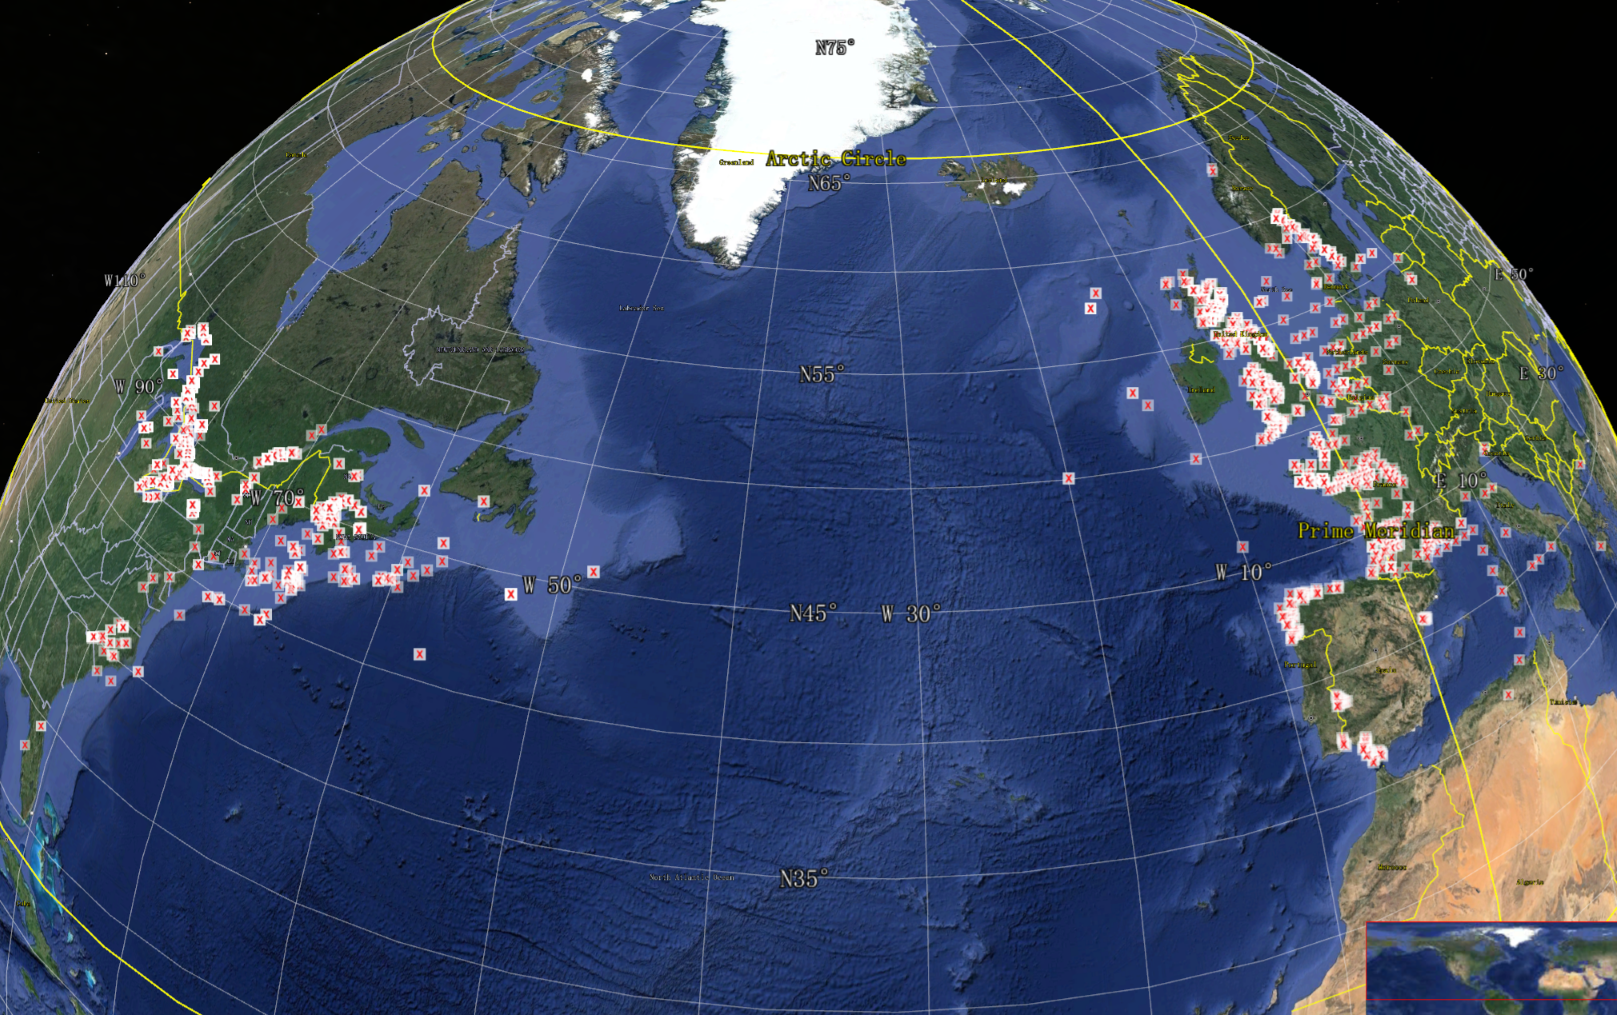
\includegraphics[width=.9\textwidth]{img/distribution.png} %图片的名称或者路径之中有空格会出问题 
		\caption{Worldwide distribution of lamprey.(The more red dots, the more dense the distribution.)} % 图片标题 
		\label{fi:1}
	\end{figure}
	\vspace{-0.8cm}
	
\subsection{Restatement of the Problem}

\begin{itemize}
	\setlength{\parsep}{0ex} %段落间距
	\setlength{\topsep}{2ex} %列表到上下文的垂直距离
	\setlength{\itemsep}{1ex} %条目间距
	\item %建立一个数学模型,预测七鳃鳗数量及性别比例变化对生态系统的影响。
	Establish a mathematical model to forecast how changes in lamprey populations and sex ratios would affect the environment.
	\item %探索七鳃鳗种群特性,分析性别比例变化使该种群更具有适应性还是更不稳定
	Explore the features of the lamprey population and determine if changes in sex ratios have made it more adaptable or unstable.
	\item %扩展模型,建立生态系统稳定性指标,分析七鳃鳗性别比例变化对该指标的影响
	By expanding the model, one may create an ecological stability index and investigate the effects of changes in the lamprey sex ratio on it.
	\item %考虑七鳃鳗性别比例变化和其他生物种群的相互作用,是否会对其他物种产生积极影响
	Examine how changes in the sex ratio of lamprey interact with other biological populations to see whether there will be benefits for other species.
\end{itemize}


 \subsection{Our Work}%还不知道怎么写
We gradually build three mathematical models in accordance with the requirements.As demonstrated below.
%这个图片用来站个位置
 \begin{figure}[htbp]  %h此处,t页顶,b页底,p独立一页,浮动体出现的位置
	\centering  %图表居中
	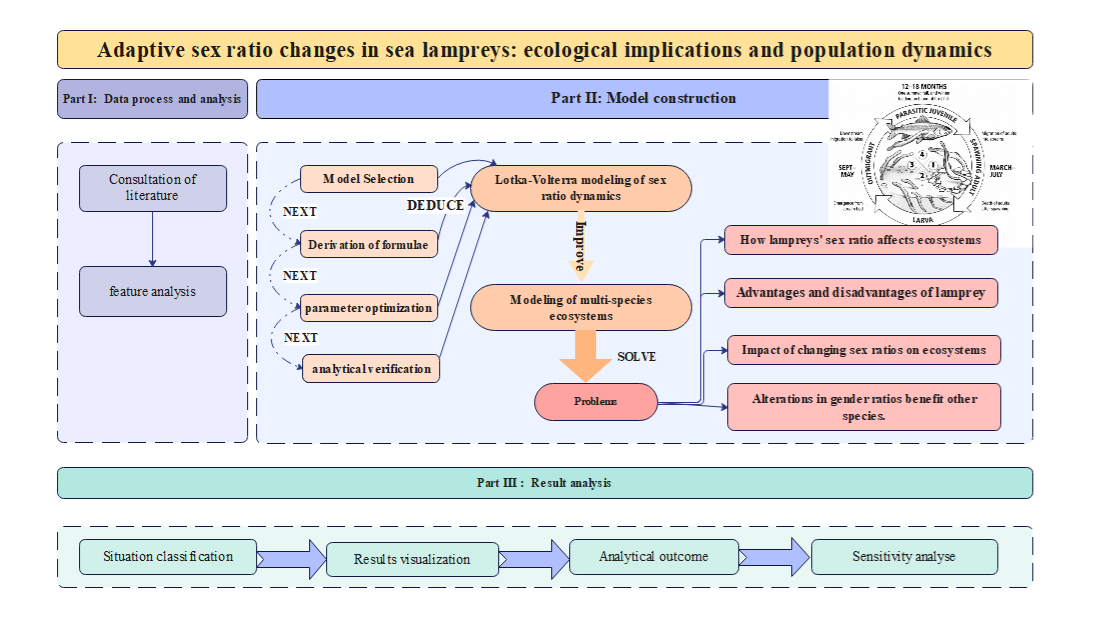
\includegraphics[width=.9\textwidth]{img/our work.png} %图片的名称或者路径之中有空格会出问题 
	\caption{Our work} % 图片标题 
\end{figure}
\vspace{-0.8cm}
\begin{comment}
\begin{enumerate}[\bfseries 1.]
	\setlength{\parsep}{0ex} %段落间距
	\setlength{\topsep}{0.5pt} %列表到上下文的垂直距离
	\setlength{\itemsep}{0.5pt} %条目间距
	\item Based on the data of wildfires, a rasterized Multi-Objective Optimization Model is established;
	\item The mixture of the two drones is given and the extreme fire events is considered;
	\item Based on the verification model simulated by Poisson process and the hovering model based on Tabu Search, this article effectively demonstrates the validity and applicability.
\end{enumerate}
\end{comment}
%这里放图片
 \section{Assumptions and Explanations}
 %考虑到实际问题的复杂性,提出如下假设进行简化,每一个都是合理地
 Considering the complexity of the actual problem, the following assumptions are proposed for simplification, each of which is justifiable:

\begin{enumerate}[\bfseries \textit{Assumption} 1:]
	\item \textbf{%不区分不稳定的性别决定和性别逆转,将性别决定和性别逆转的过程合在一起。
	The process of gender decision-making and gender reversal is combined without distinction between unstable gender decisions and genuine reversals.}\\
	\textbf{\textit{Justification: }}%受环境影响,性别决定在进入寄生期之前不稳定.
	Environmental factors impact sex determination up until the parasitism stage.\upcite{2}
	\item \textbf{%幼虫性别决定仅由环境因素决定,不考虑其他因素
	Larval sex determination is determined by environmental factors alone, regardless of other factors.}\\
	\textbf{\textit{Justification: }}
	%生物和非生物因素被认为有助于七鳃鳗物种的性别决定,如幼虫密度、温度、pH值,以及生理资源何时被转移到体细胞生长,尽管机制尚未得到很好的确定
	Biotic and abiotic factors are thought to contribute to sex
	determination in lamprey species, such as larval
	density, temperature, pH, and when physiological
	resources are diverted into somatic growth, although mechanisms are not well established.\upcite{1}
	\item \textbf{%不存在人为因素干预,例如杀虫剂、人为结构广泛破坏河流系统,减少纵向连通性,抑制了洄游
	Absence of anthropogenic interventions such as pesticides, substantial disruption of river systems by manmade constructions, loss of vertical connection, suppression of migration.}\\
	\textbf{\textit{Justification: }} %本模型主要研究七鳃鳗种群和自然生态系统的相互作用,应尽量减少人为干预
	Because this model focuses on the relationships between natural ecosystems and lamprey populations, we should reduce the amount of human involvement.
	\item \textbf{%群落中物种之间的竞争或互利关系保持不变
	Competitive or mutually beneficial relationships between species in the community remain constant.}\\
	\textbf{\textit{Justification: }}%认为短期内,生物之间相互作用关系保持不变
	It is believed that in the short term, biological interactions remain unchanged.
	\item \textbf{%物种不会变异,种群及其控制的资源会随着时间而变化
	Species do not mutate, populations and the resources they control change over time.}\\
	\textbf{\textit{Justification: }}%本模型中,资源及其控制资源是变量
	In this model, resources and the resources they control are variables.
	\item \textbf{%生长速度对性别的影响系数是固定的,不随时间或空间变化
	The coefficient of growth rate on sex is fixed and does not vary over time or space.}\\
	\textbf{\textit{Justification: }}%根据[1],此系数目前尚未确定,暂时假定为固定的
	According to \upcite{1}, the mechanisms are not well established, Temporarily assumed to be fixed.
	\item \textbf{%雄雌的死亡率影响因素相同
	Male and female mortality rates are affected by the same factors.}\\
	\textbf{\textit{Justification: }}%性腺发育期间更高的能量需求对雌性死亡率的影响较小,因此不考虑这些因素
	These characteristics are not taken into account since higher energy requirements during gonadal development have a lower influence on female mortality. 
	\item \textbf{%假设寄生虫的寄生行为视作周期更长、死亡率更低的捕食行为
	Considering that a parasite's activity is considered to be a form of longer-lasting and less lethal predation.}\\
	\textbf{\textit{Justification: }}%大部分寄生虫会摄取寄主养分,并传播病菌,长期来看,增加了宿主死亡概率,因此这样假设
	It is believed that most parasites absorb resources from their hosts and spread infections, which raises the likelihood of host mortality over time.
	\item \textbf{%假设不同性别的七鳃鱼在面对寄生虫的寄生行为时有相同表现,即致死率、被捕食率等指标相同。
	When faced with the parasitic activity of the parasite, lamprey of various sexes exhibit the identical behaviors, i.e., the same markers of lethality and predation rate.}\\
	\textbf{\textit{Justification: }}%寄生虫对lamprey性别选择目前并未得到研究,为了简化模型,这里假设相同
	Parasite sex selection on lamprey is not currently studied, and to simplify the model, the same is assumed here.
	\item \textbf{%假设生态系统中七鳃鳗不被任何物种捕食,寄生虫的寄生行为除外,人类偷猎造成的
	Considering that no creature in the environment preys on lamprey, other from parasitism by parasites, and that human hunting results from.}\\
	\textbf{\textit{Justification: }}%七鳃鳗的因捕食而造成的死亡占其总死亡的极少部分
	Only a very tiny percentage of lamprey overall mortality is caused by predator-related causes.
	
	
	
\end{enumerate}
Additional assumptions are made to simplify analysis for individual sections. These assumptions will be discussed at the appropriate locations.

\section{Notations}
Some important mathematical notations used in this paper are listed in Table 1. 
\begin{table}[htbp]
	\begin{center}
		\caption{Notations used in this paper}
		\begin{tabular}{c l}
			\toprule[2pt]
			\multicolumn{1}{m{3cm}}{\centering Symbol}
			&\multicolumn{1}{m{8cm}}{\centering Description }\\
			\midrule
			$k_1$& %食饵的自增长率
			Self-growth rate of preys \\
			$k_2$& %捕食者的负自增长率
			Negative self-growth rate of predators \\
			$b$& %捕食者对食饵的掠食能力
			The capacity of the predator to consume prey\\
			$c$& %食饵对捕食者的供养能力。
			The bait's capacity to nourish the predator\\
			$x$ & Population size of the prey \\
			$y$ & Population size of the predator \\
			$Y_1$ & Population size of the predator \\
			$Y_2$ & Population size of the prey\\
			$r_1$ & Endogenous growth rate of predator\\
			$r_2$ & Endogenous growth rate of and prey\\
			$K_1$ & Predators' environmental carrying capacities\\
			$K_2$ &Prey's environmental carrying capacities\\
			
			
			\bottomrule[2pt]
		\end{tabular}\label{tb:notation}
		\begin{tablenotes}
			\footnotesize
			\item[*] *There are some variables that are not listed here and will be discussed in detail in each section. %此处加入注释*信息
		\end{tablenotes}
	\end{center}
\end{table}
\vspace{-1cm}%在\end{table}下加一行\vspace{-1cm} 其中-1的作用是缩短与下方文字距离的 切记!必须是负数

\section{Model Establishment and Solution}
\subsection{%基于Volterra食饵-捕食者的模型建立
Volterra Modeling Based on  Prey-Predator}


\subsubsection{The establishment of model}
%自然界中不同种群之间存在捕食这种既有依存、又有制约的生存方式:种群甲靠丰富的自然资源生长,而种群乙靠捕食种群甲为生:生态学上称种群甲为食饵(Prey),种群乙为捕食者(Predator),二者组成食饵-捕食者系统,又称P-P系统。
In the natural world, predation is a means of survival that involves both constraints and dependence. For example, population A depends on an abundance of natural resources to grow, while population B depends on predation on population A to survive. In terms of ecology, this is known as the bait-predator system, or P-P system, wherein population A is the predator and population B is the prey.\par
%在只考虑食物资源可用性的情况下,没有捕食者,食饵净相对增长率为正常数,没有食饵,捕食者的净相对增长率为负常数,两类物种相遇的机会正比于它们的数量乘积,模型如式:
When only the availability of food resources is taken into account, there are no predators, preys net relative growth rate is a normal number. While there are no preys, predators net relative growth rate is a negative constant, and the likelihood of two species coming into contact is determined by the product of their populations, as represented by Equation \ref{eq:11}:
\begin{equation}
	\begin{cases}
		\begin{aligned}
			\frac{dx}{dt} &= k_{1}x - bxy = x(k_{1} - by) \\
			\frac{dy}{dt} &= -k_{2}y + cxy = y(-k_{2} + cx)
		\end{aligned}
		\label{eq:11}
	\end{cases}
\end{equation}
%在不考虑性别差异的情况下,物种受环境承载力等实际因素影响,Volterra捕食者-猎物系统模型如式:
\par
Without considering sex differences, species are influenced by practical factors such as environmental carrying capacity, and the Volterra prey-predator system is modeled as Equation \ref{eq: 2}:

\begin{equation}
	\begin{cases}
		\begin{aligned}
			\frac{dY_1}{dt} &= r_1 Y_1 \left(1 - \frac{Y_1 + \alpha_{12} Y_2}{K_1}\right) - \beta_{12} Y_1 Y_2\\
			\frac{dY_2}{dt} &= r_2 Y_2 \left(1 - \frac{Y_2 + \alpha_{21} Y_1}{K_2}\right) - \beta_{21} Y_1 Y_2
		\end{aligned}
		\label{eq: 2}
	\end{cases}
\end{equation}
\par
%由于lamprey具有独特的性别变化规律,幼虫的生长速度会影响物种性别比例,因此需要考虑性别比例变化对七鳃鳗带来的影响
Because lamprey has a unique pattern of sex change. Sex determination in sea lamprey is directly influenced by larval growth rate.\upcite{2} Thus, it is necessary to take the gender ratio's effects into account.\par

%定义性别比例$R_{\sigma}$为雄性的数量与种群总数的比值:
Define the sex ratio $R_{\sigma}$ as the ratio of the number of males to the total population:
\begin{equation}
	\begin{aligned}
	R_{\sigma} &=\frac{male\_number}{female\_number+male\_number}
	\end{aligned}
	\label{eq:gender_ratio}
\end{equation}

%定义$R(A)$为性别决定比率关于食物资源可用性A的变化,如下式所示。当食物资源缺少时,雄性比例增加;食物资源充沛时,雄雌比例接近均衡。
Define $R(A)$ as the change in sex determination  ratio with respect to the availability of food resources, A, as shown in the following equation \ref{eq:1}. When food resources are scarce, the proportion of males increases; when food resources are plentiful, the proportion of males and females approaches equilibrium.
\begin{equation}
	R(A) = \alpha \ln\left(A + \beta \right)+\gamma \label{eq:1}
\end{equation}
%食物资源量A和被捕食者群体与捕食者群体的数量比例有关:
The amount of food resource A is related to the ratio of the number of prey groups to the number of predator groups:
\begin{equation}
	\begin{aligned}
		A &=\frac{P}{\sum Y_j}
	\end{aligned}
\end{equation}

%综合上述因素后,分别对雌性和雄性lamprey进行建模,如下式:
\par
The following Equation \ref{eq: 5} represents the separate modeling of the male and female lampreys after the aforementioned elements were combined:
\begin{equation}
	\left\{
	\begin{aligned}
		\frac{dY_1}{dT} &= \left(1 - \frac{Y_1 + Y_2}{k_1}\right) \left[ \sigma  \frac{Y_1 Y_2}{Y_1 + Y_2} \cdot R_a -  \text{death\_rate} \cdot Y_1\right] + m \cdot R_a  \\	
		\frac{dY_2}{dT} &= \left(1 - \frac{Y_1 + Y_2}{k_1}\right) \left[\sigma \frac{Y_1 Y_2}{(Y_1 + Y_2)^2} (Y_1 + Y_2) \right. \left. (1 - R_a) - \text{death\_rate} \cdot Y_2 \right] + m \cdot (1 - R_a) \\				
		\frac{dY_3}{dT} &= \text{prey\_add} \cdot Y_3 \left(1 - \frac{Y_3}{k_2}\right) - \text{preyed\_rate} \cdot Y_3 (Y_1 + Y_2)\\
		R_a &= -0.1514\ln\left(\frac{Y_3}{Y_1 + Y_2} + 0.4585\right) + 0.7569  \\
		m &= \text{preyed\_rate} (male\_prate \cdot Y_1 + female\_prate \cdot Y_2) \cdot Y_3 \\
	\end{aligned}
	\label{eq: 5}
	\right.
\end{equation}
%其中,$Y_1$表示雄性lampreys数量,$Y_2$表示雌性lampreys数量,$Y_3$表示猎物的数量,将雌雄性别分别进行建模,可以使得物种可用性导致的性别变化对种群的真实性别比例的影响存在滞后性
The three numbers are $Y_1$, $Y_2$, and $Y_3$, which represent the number of male, female, and prey items, respectively.Modeling the male and female sexes separately, which make it possible to make a lag in the effect of sex changes due to species availability on the true sex ratio of a population.

\subsubsection{%使用模型进行预测
	Model-based prediction}
	%本文模拟的生态环境演化总时间长度为1000,时间步长为0.5此外,根据资料【参考论文】,lampreys在五大湖地区属于外来物种入侵,不存在天敌。这里为了简化问题,考虑群落里有两个物种,分别是sea lampreys和被他捕食的食饵。根据假设,生长速度只和食物资源可用性有关。在幼虫时期lampreys以浮游生物和碎屑为食,在这个过程中受捕食情况的影响确定性别比例。
This article uses a time step of 0.5 and a total duration of 1000 to model ecological development. Furthermore, there are no natural adversaries for lampreys, which are an invasive foreign species in the Great Lakes region, according to \upcite{2}. Here, to make things easier, think of two species in the community: sea lampreys and the bait that they eat.Larvae remain burrowed for 3–5 years on average, and filter-feed on seston,diatoms, and biofilm.\upcite{3} Sex ratios are determined in a process influenced by predation.\par
%合理估计出微分方程模型中其他系数的定量值,如表所示。具体的数值可以通过实地调查或文献来获得。
The table presents a reasonable approximation of the quantitative values of the other coefficients in the differential equation model. Field surveys and published works can provide specific values.


\begin{table}[htbp]
\begin{center}
	\caption{Values of the Model Assumptions Parameters}
	\resizebox{\textwidth}{!}
	{\begin{tabular}{c c}
			\toprule[2pt]
			\multicolumn{1}{m{8cm}}{\centering \textbf{Parameters}}
			&\multicolumn{1}{m{5cm}}{\centering \textbf{Initial Value} }\\ %m后面是列宽
			\midrule
			Birth rate(birth\_rate) & 0.15 \\
			Mortality rate(death\_rate) & 0.20 \\
			Male predation efficiency(male\_prate) & 0.4 \\
			Female predation efficiency(female\_rate) & 0.38 \\
			Probability of prey being attacked by predators (preyed\_rate) & 0.0006 \\
			Prey natural increase rate(prey\_add) & 0.1 \\
			Lampreys' environmental carrying capacities(k1) & 5000\\
			Prey's environmental carrying capacities(k2) & 5000\\
			Initial male count($x_0\_male$) & 50 \\
			Initial female count($x_0\_female$) & 50 \\
			Initial prey count($x_0\_prey$) & 500 \\
			Debugging parameters($\sigma$) & 0.56 <= $\sigma$ <= 0.64  \\
			\bottomrule[2pt]
	\end{tabular}}
\end{center}
\end{table}


\begin{figure}[htbp]
	\begin{minipage}[b]{0.5\linewidth}
		\centering
		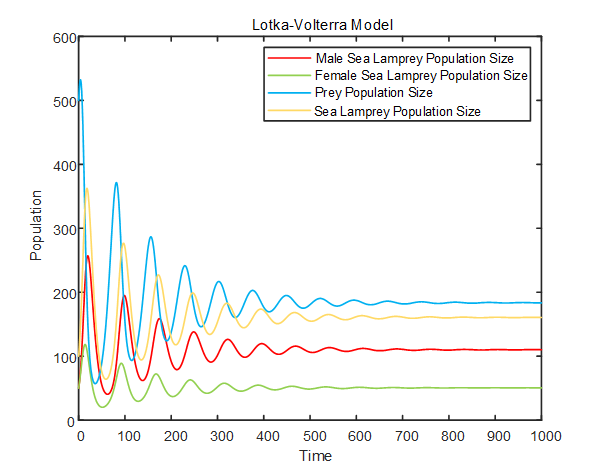
\includegraphics[width=\linewidth]{img/Lotka-Volterra Model.png}
		\caption{Lotka-Volterra Model}
	\end{minipage}%
	\begin{minipage}[b]{0.5\linewidth}
		\centering
		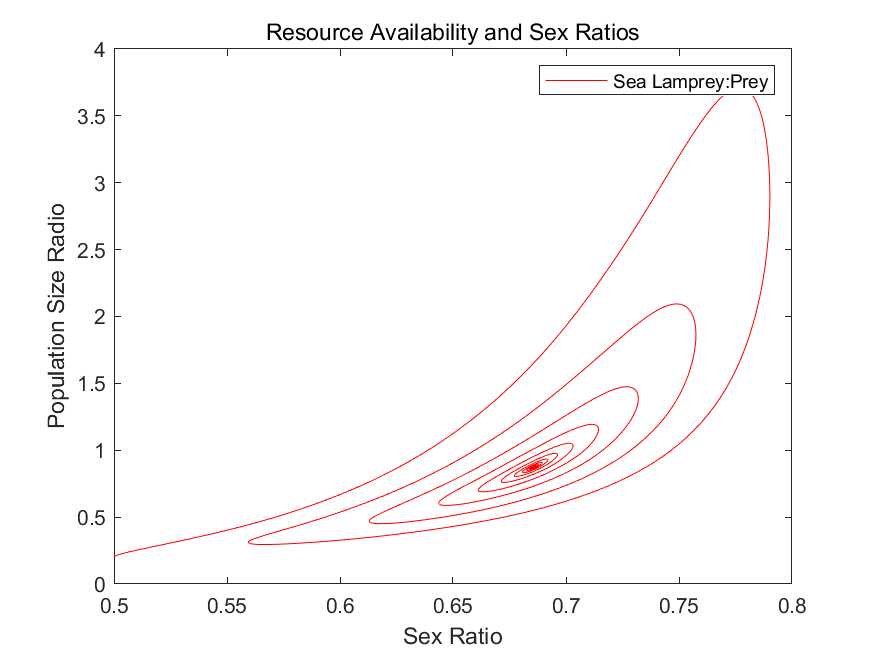
\includegraphics[width=\linewidth]{img/Resource Availability and Sex Ratios.png}
		\caption{Resource Availability and Sex Ratios}
	\end{minipage}
\end{figure}

%从图3,图4中可以得出sea lampreys的数量变化,食物资源可用性和性别比例的关系
	Variations in the number of sea lampreys, availability of food resources and gender ratio can be inferred from Figure 3, Figure 4. \par
%在图3中,lampreys和prey的数量呈现周期性变化,并逐渐趋于稳定。由于不存在天敌,lampreys的数量在初始条件下会增加,对应prey数量急剧下跌。当prey数量呈现下降趋势时,由于食物资源可用性降低,lampreys的数量不会立刻随之变化而是滞后下降。这是因为猎物数量增加时lampreys数量增加需要时间,猎物减少时也不会使捕食者立刻饿死导致死亡率立即明显升高。最终由于这种制约和依存关系 ,导致数量呈现周期性变化并趋于稳定。
The populations of prey and lampreys in Figure. 3 fluctuate periodically before steadily stabilizing. Under initial conditions, there is a dramatic reduction in the amount of prey, which corresponds to an increase in lamprey numbers due to the absence of natural adversaries. Because there are less food supplies available to them, lamprey populations drop with a lag rather than an instantaneous response when the prey population declines. This is due to the fact that an increase in prey does not immediately result in the predator starving to death, which would imply an abrupt and substantial rise in mortality. Rather, an increase in prey takes time for the number of lampreys to grow. Ultimately, cyclical fluctuations and population stabilization result from these limitations and interdependence.\par
%在图四中,展示了食物资源和lampreys性别比例的变化关系。当食物资源丰富时,性别比例接近0.5的均匀性别比例,而食物资源缺乏时,雄性比例会明显增加。这样的变化情况与实际情况相符。
Figure 4 depicts how the sex ratio of lampreys and food supplies change throughout time. When food resources are abundant, the sex ratio is close to the even sex ratio of 0.5, whereas when food resources are scarce, the proportion of males increases significantly. Such a variation is consistent with the actual situation. \par
%这种变化是可以解释的,例如在生长受限的情况下,由于性腺发育期间更高的能量需求,雌性可能会经历更高的死亡率。雄性可能减少了对食物资源的总体需求。雌性和雄性在捕食中可能对资源利用有不同效率,雄性对资源利用率更高,导致生长所需要的食物资源比雌性更少。
These alterations can be explained, for instance, by the possibility that in cases of growth limitation, female mortality may be greater because of the increased energy requirements during gonadal development. It's possible that men have decreased their total need for food supplies. Males may use resources more efficiently than females when it comes to predation, meaning that less food resources are needed for development in the male than in the female.
\subsection{Further Model Analysis} %解决问题2
\subsubsection{%适应性性别比例变化带来的优势和劣势
Advantages and disadvantages associated with adjustments to the adaptive sex ratio}
%为了探究性别比例变化给lampreys带来的优势和劣势,考虑改进Volterra捕食者-猎物系统模型,在模型中忽略性别比例对捕食效率,繁殖成功率的影响,即不存在适应性性别比例变化的情况。建立如下方程:
Consider enhancing the Volterra predator-prey system model by excluding the impact of sex ratio on predation efficiency and reproductive success, i.e., there is no adaptive sex ratio change, in order to investigate the benefits and drawbacks of sex ratio changes for lampreys. \par
%考虑性别区分,参照前面建立的Equation4
Taking the gender difference into account, see the previously stated Equation(4) .\par
%不考虑性别区分
The following Equation(5), which disregards gender differences, is as followed:
\begin{equation}
	\left\{
		\begin{aligned}
			\frac{dx_1}{dt} &= \left(1 - \frac{x_1}{k_1}\right) \cdot x_1 \left(0.25 \sigma - \text{death\_rate}\right) + 0.5 n  \cdot \text{preyed\_rate} \cdot x_1 \cdot x_2 \\
			\frac{dx_2}{dt} &= \left(1 - \frac{x_2}{k_2}\right) \text{prey\_add} x_2 - \text{preyed\_rate}\cdot x_1 \cdot x_2 \\
			n &= \text{male\_prate} + \text{female\_prate} \\
		\end{aligned}
		\right.
	\end{equation}
%假设存在一种物种与lampreys除适应性性别比例变化外习性完全相同,让这两种物种在相同的初始情况下对比种群发展趋势。我们单独饲养它们而不考虑种间竞争。通过比较高捕食率带来的种群增长速度过快,种群环境承载力过低,以及初始食物资源不足三种情况下两类物种的发展趋势,以得出优缺点分析的结论。
\par
Under the same initial conditions, assuming that there exists a species with identical habits to lampreys except for variations in adaptive sex ratios, let the two species compare population trends.Regardless of interspecific competition, we grow them individually. In order to derive findings for the study of strengths and weaknesses, the trajectories of the two species were compared in three scenarios: excessive population growth rate due to high predation rate, poor environmental carrying capacity of the population, and insufficient beginning food supplies.\par

%在种群环境承载力过低的情况下:
\par
In the case of low environmental carrying capacity of populations:
\begin{figure}[htbp]
	\begin{minipage}[b]{0.5\linewidth}
		\centering
		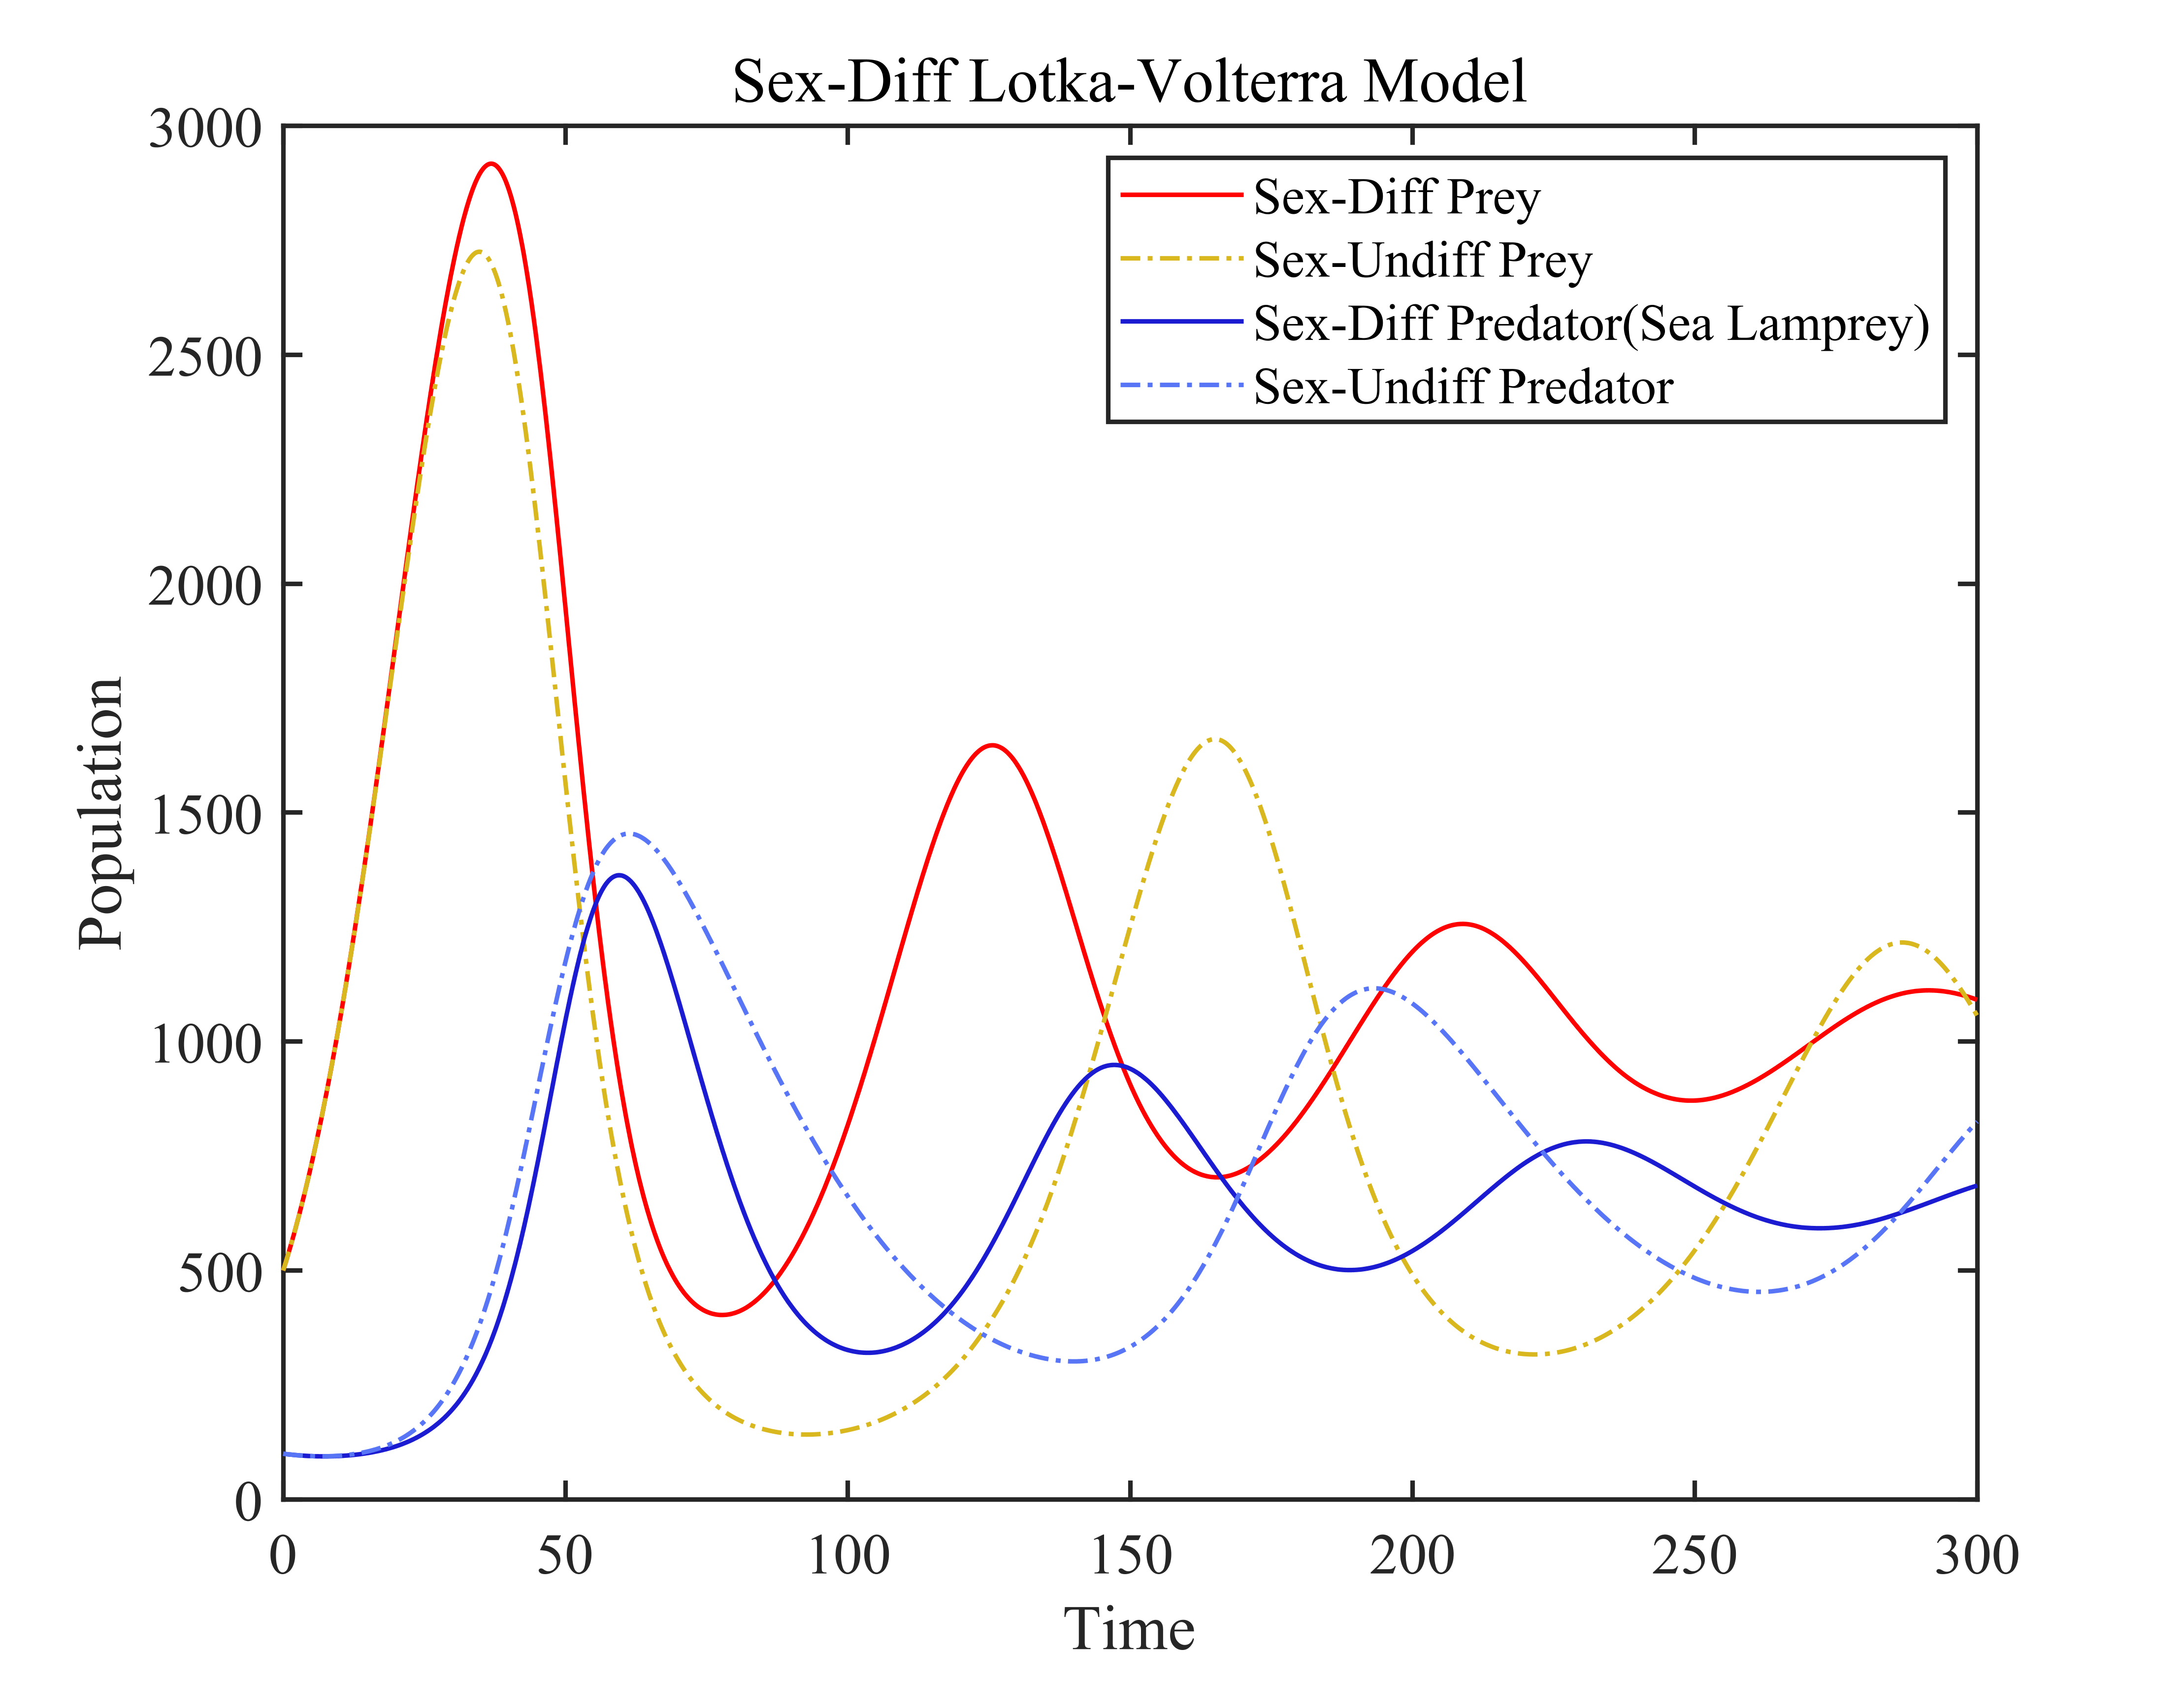
\includegraphics[width=\linewidth]{img/diff31.png}
		\caption{sex diff(low environmental capacity)}
	\end{minipage}%
	\begin{minipage}[b]{0.5\linewidth}
		\centering
		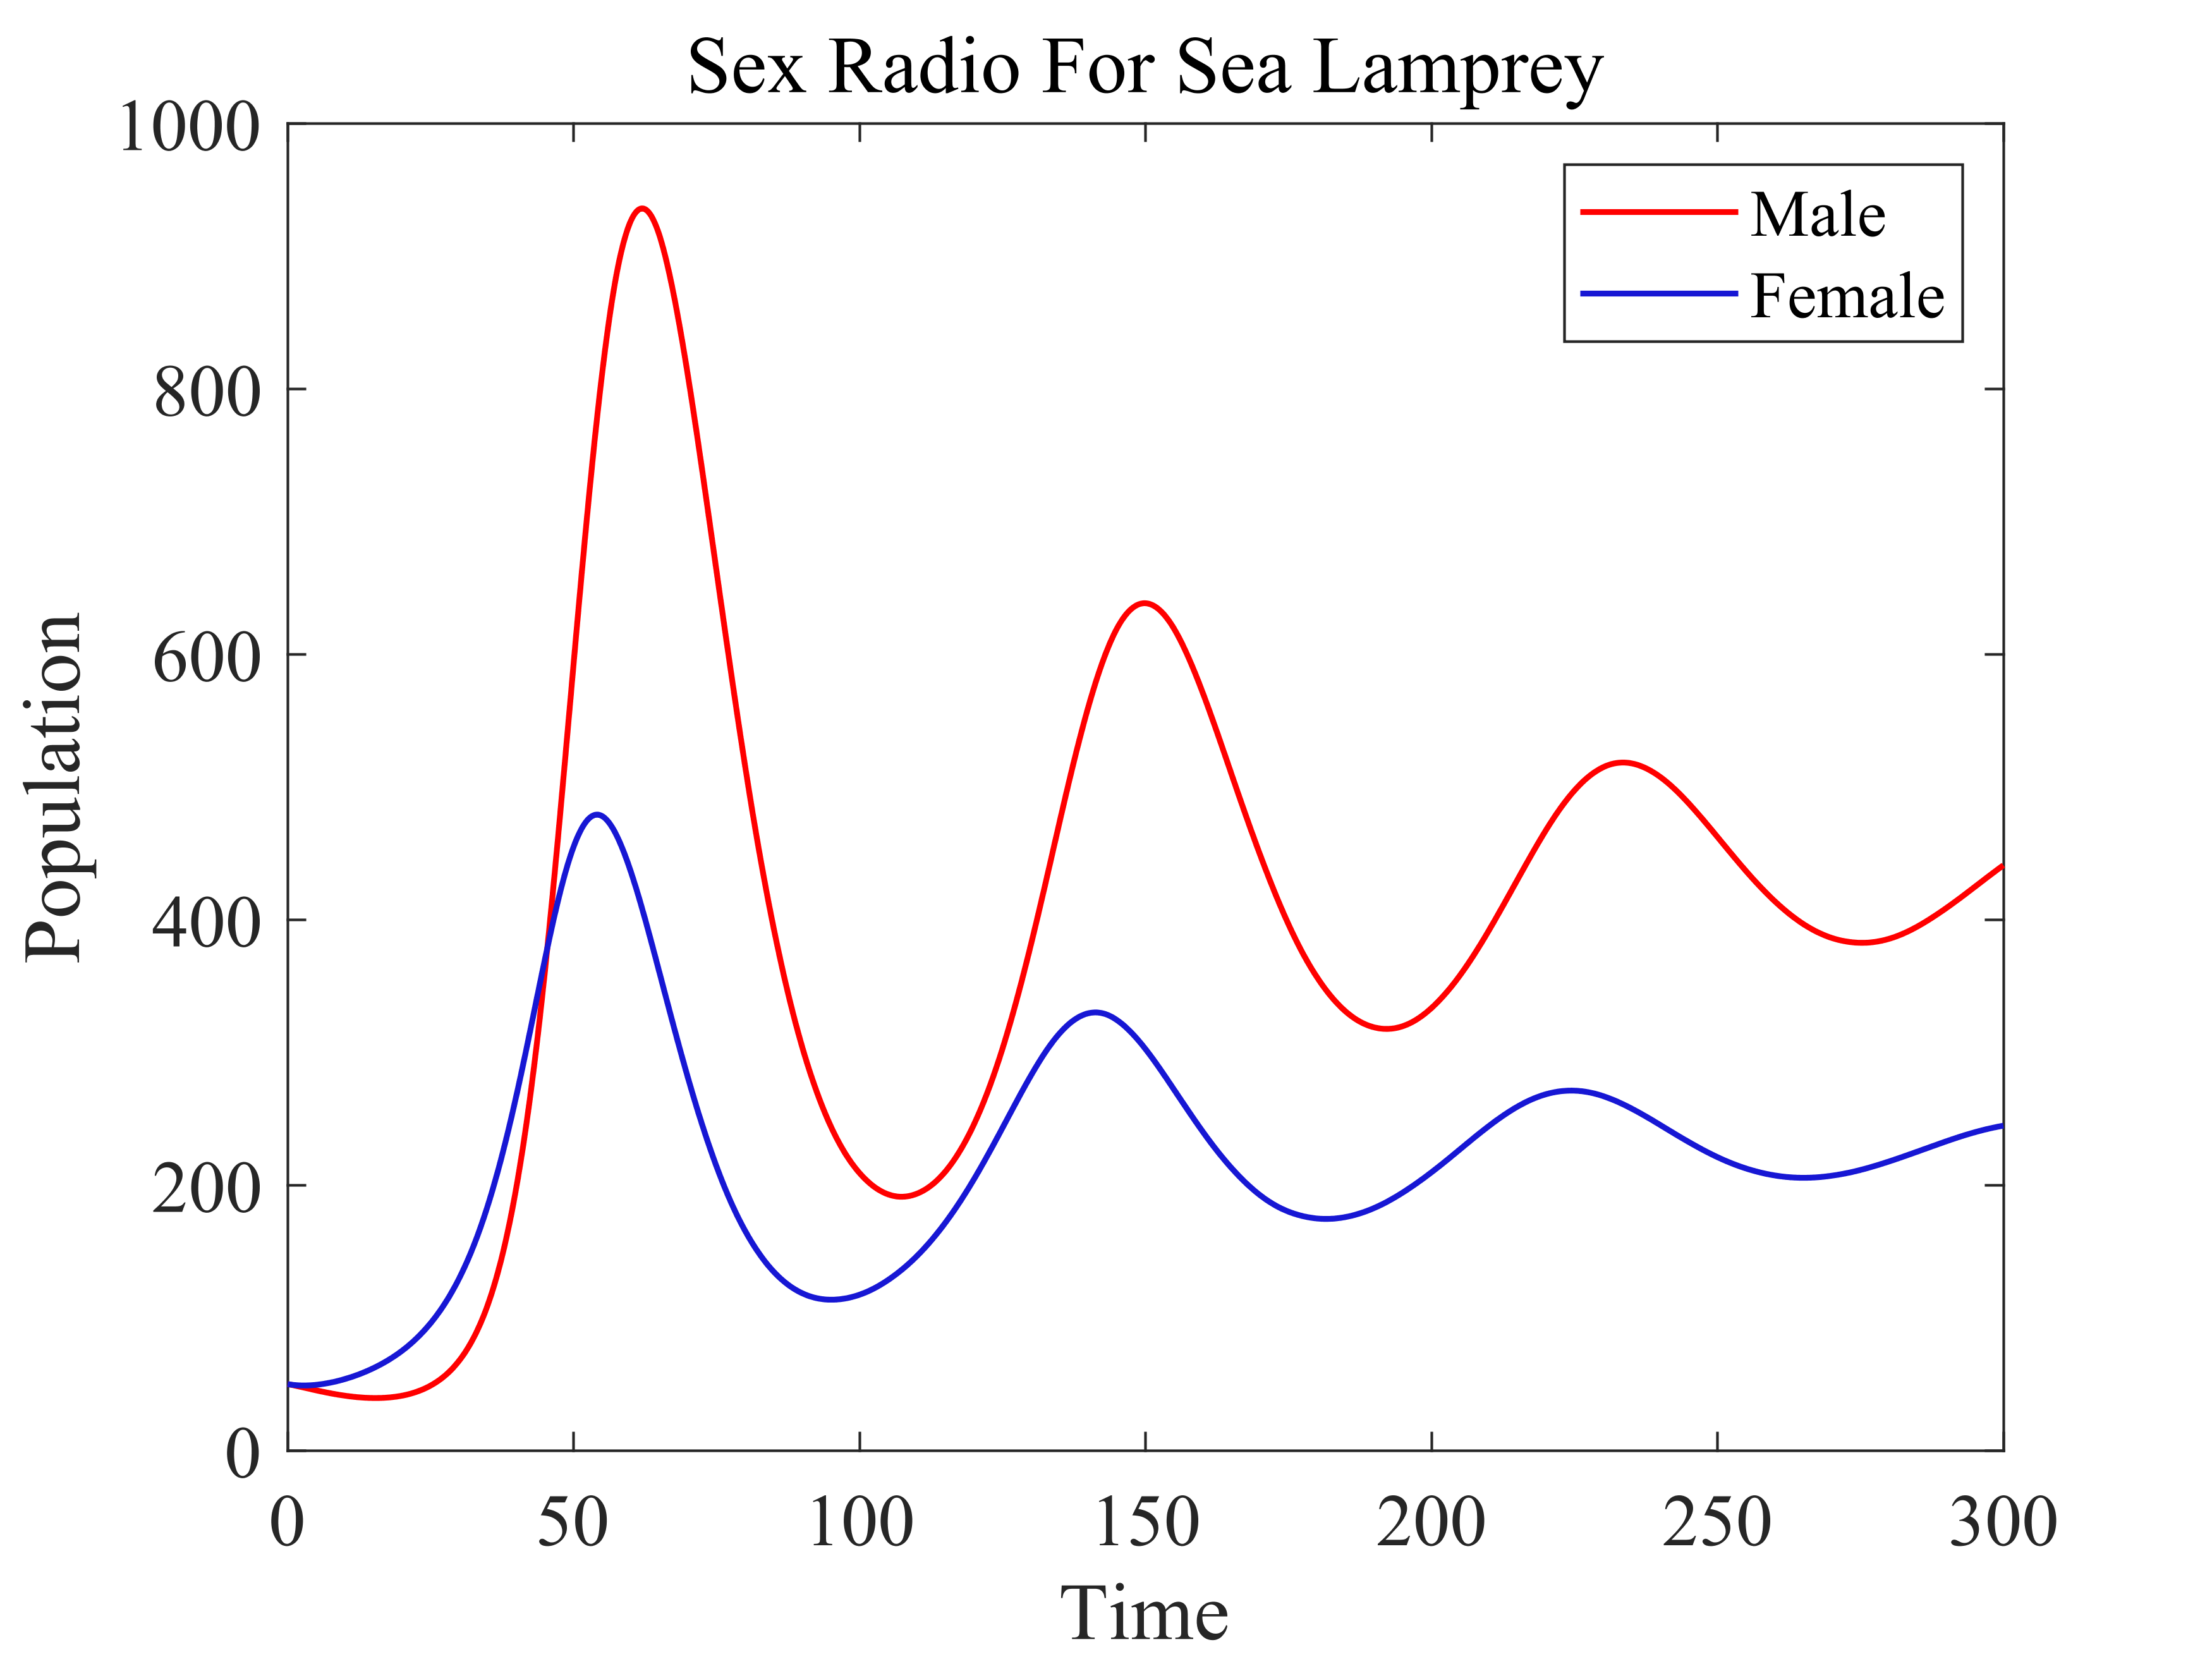
\includegraphics[width=\linewidth]{img/diff32.png}
		\caption{sex diff ratio}
	\end{minipage}
	\label{fi:3_1}
\end{figure}

%根据实验可视化结果,物种生物量呈现周期性波动,在波动过程中波动幅度逐渐降低,物种规模逐渐收敛至稳定值。lamprey波动周期更短,收敛速度更快。
According to the experimental visualization results,figure 5,figure 6, the species biomass showed periodic fluctuations, the fluctuation amplitude gradually decreased during the fluctuation process, and the species size gradually converged to a stable value. lamprey fluctuation period was shorter, and the convergence speed was faster.\par

%在高捕食率的情况下:
At high predation rates:
\begin{figure}[htbp]
	\begin{minipage}[b]{0.5\linewidth}
		\centering
		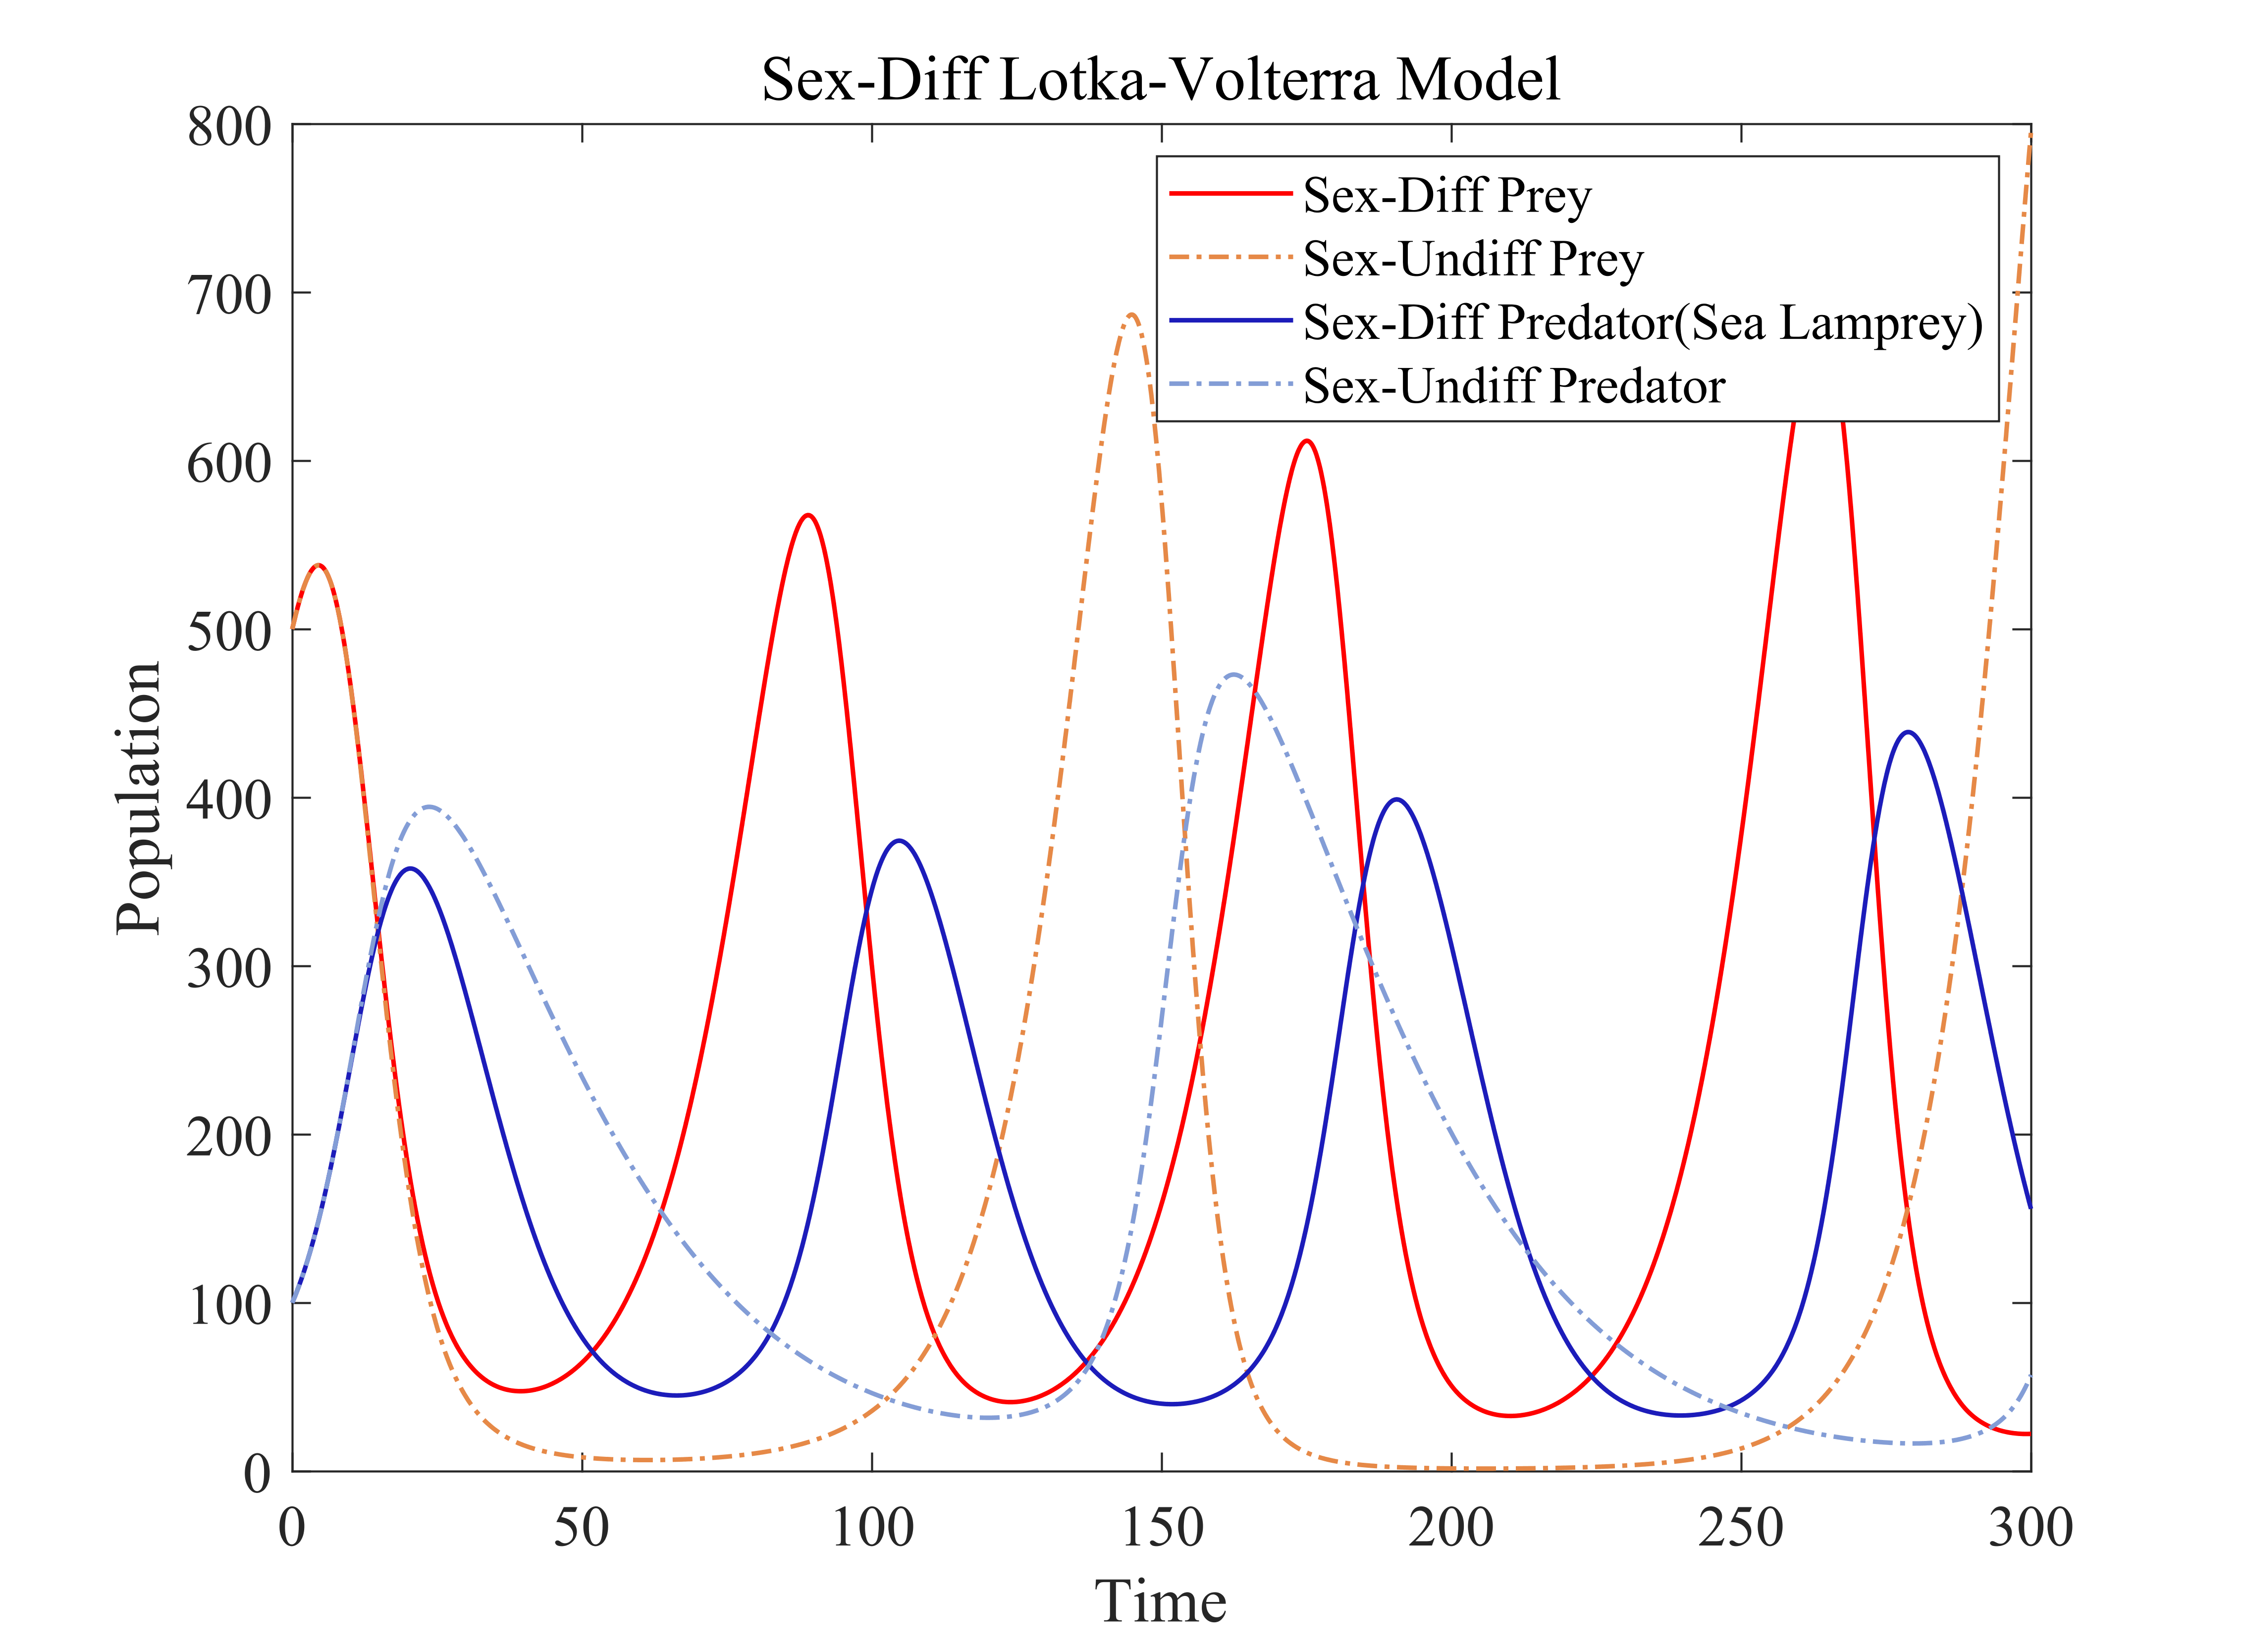
\includegraphics[width=\linewidth]{img/diff1.png}
		\caption{sex diff(high predation rate)}
	\end{minipage}%
	\begin{minipage}[b]{0.5\linewidth}
		\centering
		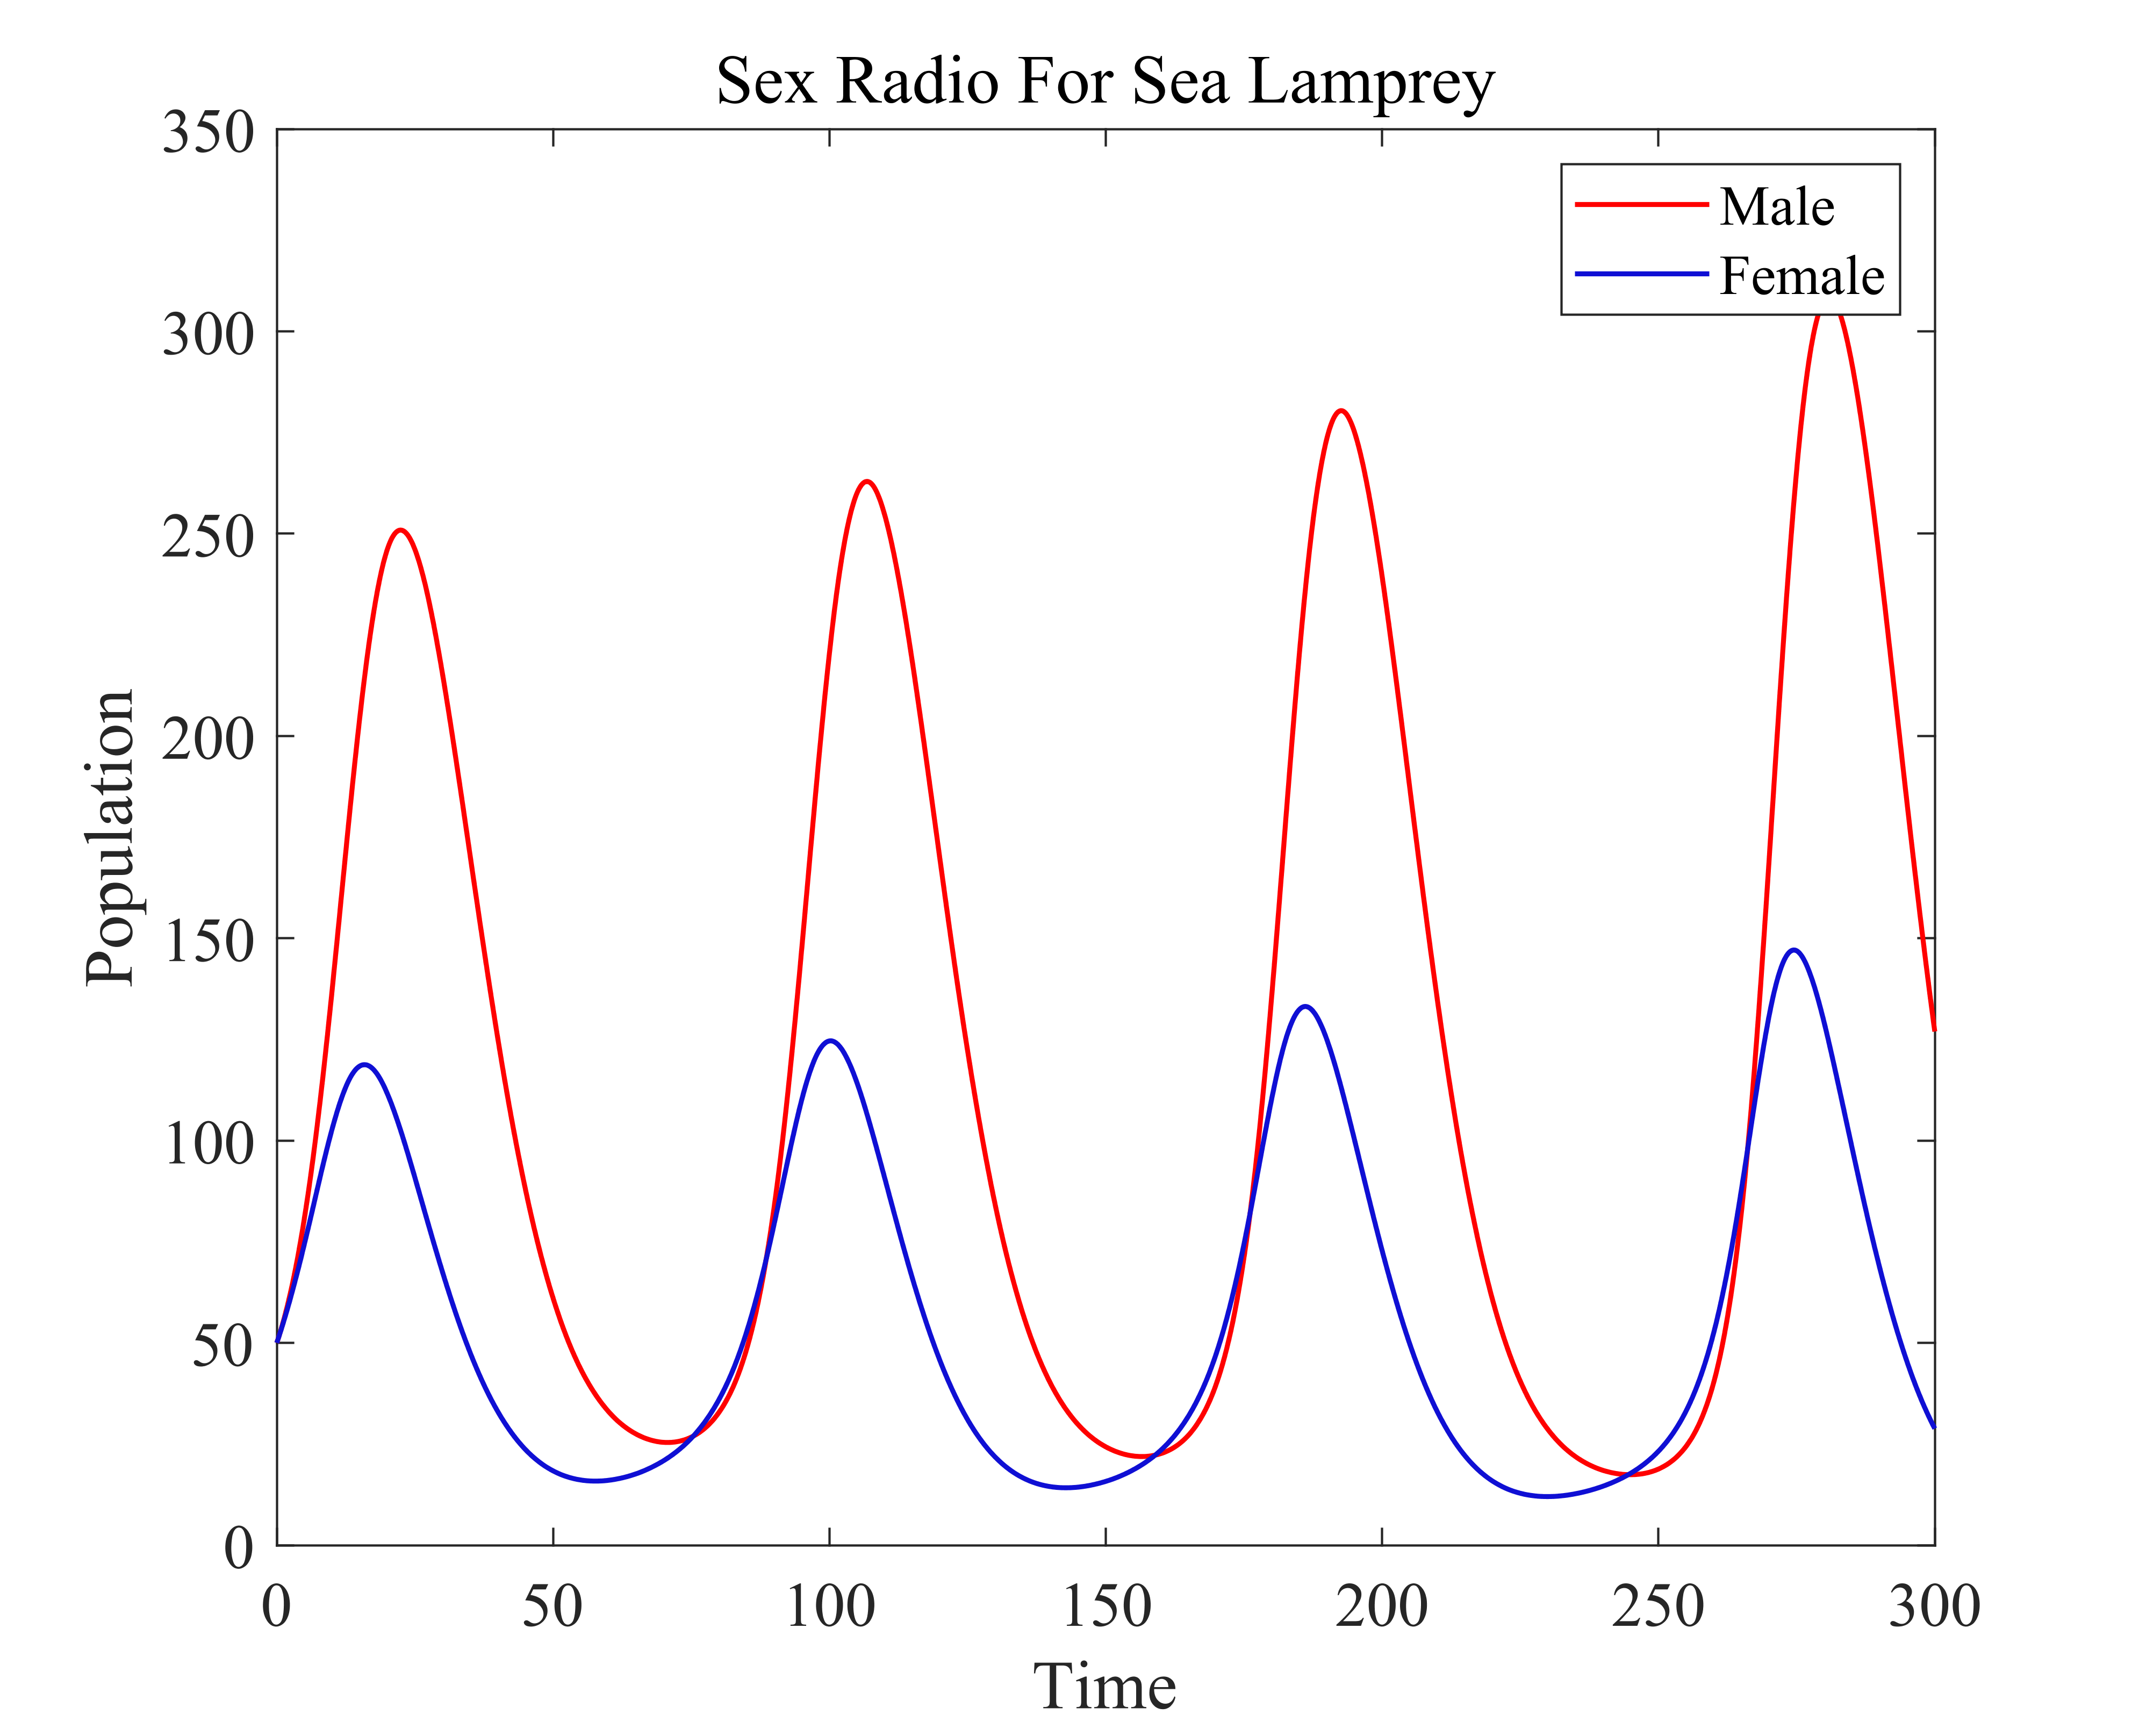
\includegraphics[width=\linewidth]{img/diff11.png}
		\caption{sex diff ratio}
	\end{minipage}
	\label{fi:3_1}
\end{figure}
\par
%在图中不难看出,lamprey对照物种种群扩张时间更长,规模更大,导致猎物的数量减少到一个难以自我恢复的值。在实际有着复杂环境因素的生态环境中,模型中贴近坐标轴的曲线可以认为该物种已濒临灭绝,而不可避免地导致以该物种为食的物种也走向灭绝。
The figure7,figure 8 makes it clear that the population of the lamprey control species has been growing for a longer time period and on a greater scale, which has caused the prey numbers to drop to a level from which it is impossible to recover. The curve along the model's axis represents a species that is in danger of going extinct, which in turn causes the extinction of the species that feeds on it in a genuine ecosystem with complicated environmental conditions.\par
%具有适应性性别比例变化的lamprey在食物减少时性别比例失衡,繁殖潜力下降,抑制了种群扩张的幅度和周期。由于性别比例的调整存在滞后性,比例失衡带来的低繁殖潜力结合食物的缺乏,使得lamprey的种群缩减,加快了猎物群体的恢复与扩张,从而让生态系统形成一个更短的迭代周期。
When food is scarce, lamprey with adaptive sex ratio modifications have unbalanced sex ratios and decreased reproductive capacity, which limits the rate and frequency of population growth. The ecosystem was able to establish a shorter iteration cycle because of the lag in sex ratio adjustment, which led lamprey populations to decline due to the poor reproductive capacity from the imbalance and the lack of food. This, in turn, expedited the recovery and growth of prey populations.\par
%在高捕食率,初始资源过于丰富或者食物的自然增长率过高 的环境下以上特点尤其突出。该情况下物种容易过度扩张造成生态系统的崩溃,而lamprey的性别变化特质可以有效抑制种群的过度扩张。造成物种灭绝是极端情况,大部分情况下这种特质表现为种群规模的周期变化幅度大,规模不稳定。
This is particularly true in settings with high rates of predation, excessively plentiful beginning resources, or excessively rapid natural food increase. Since the species in question is vulnerable to both overpopulation and ecological collapse, the lamprey's sex change characteristic effectively prevents overpopulation. Although extinction is an extreme scenario, this feature is typically accompanied by instability and significant cyclical variations in population size.\par






%在初始食物资源不足的情况下:
In case of insufficient initial food resources, the result are as followed Figures:
\begin{figure}[htbp]
	\begin{minipage}[b]{0.5\linewidth}
		\centering
		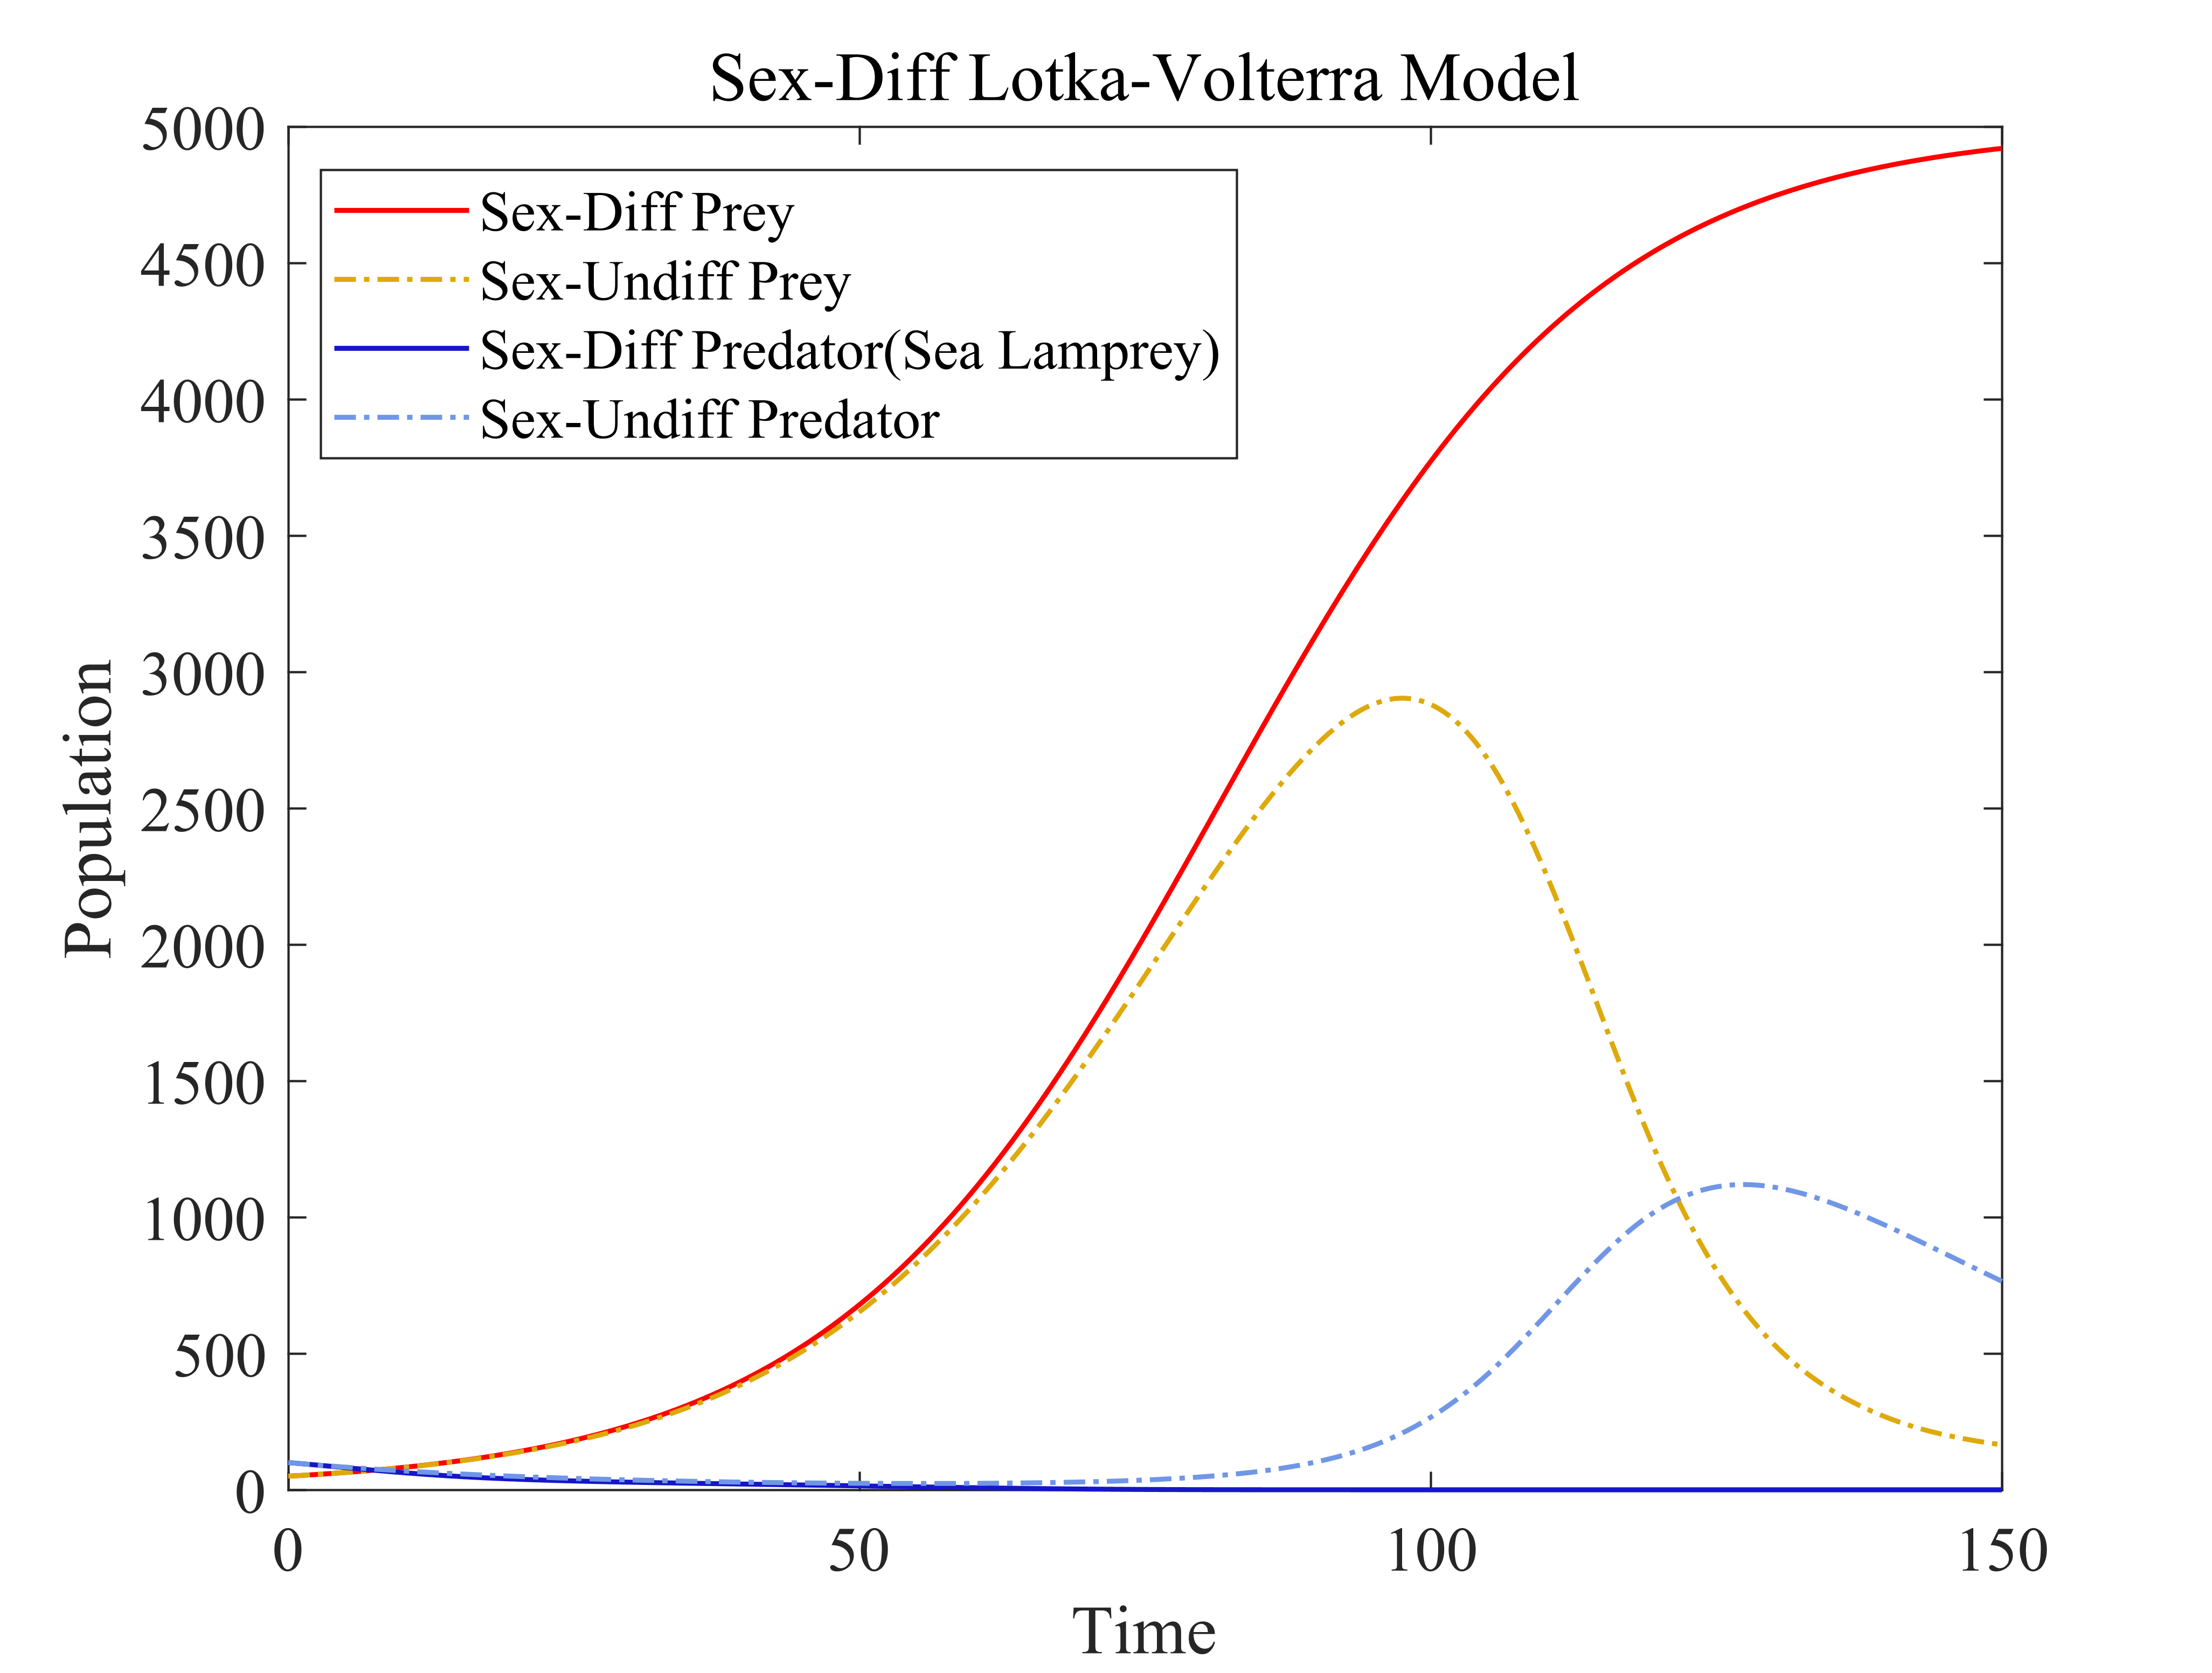
\includegraphics[width=\linewidth]{img/diff22.png}
		\caption{sex diff(low initial food)}
	\end{minipage}%
	\begin{minipage}[b]{0.5\linewidth}
		\centering
		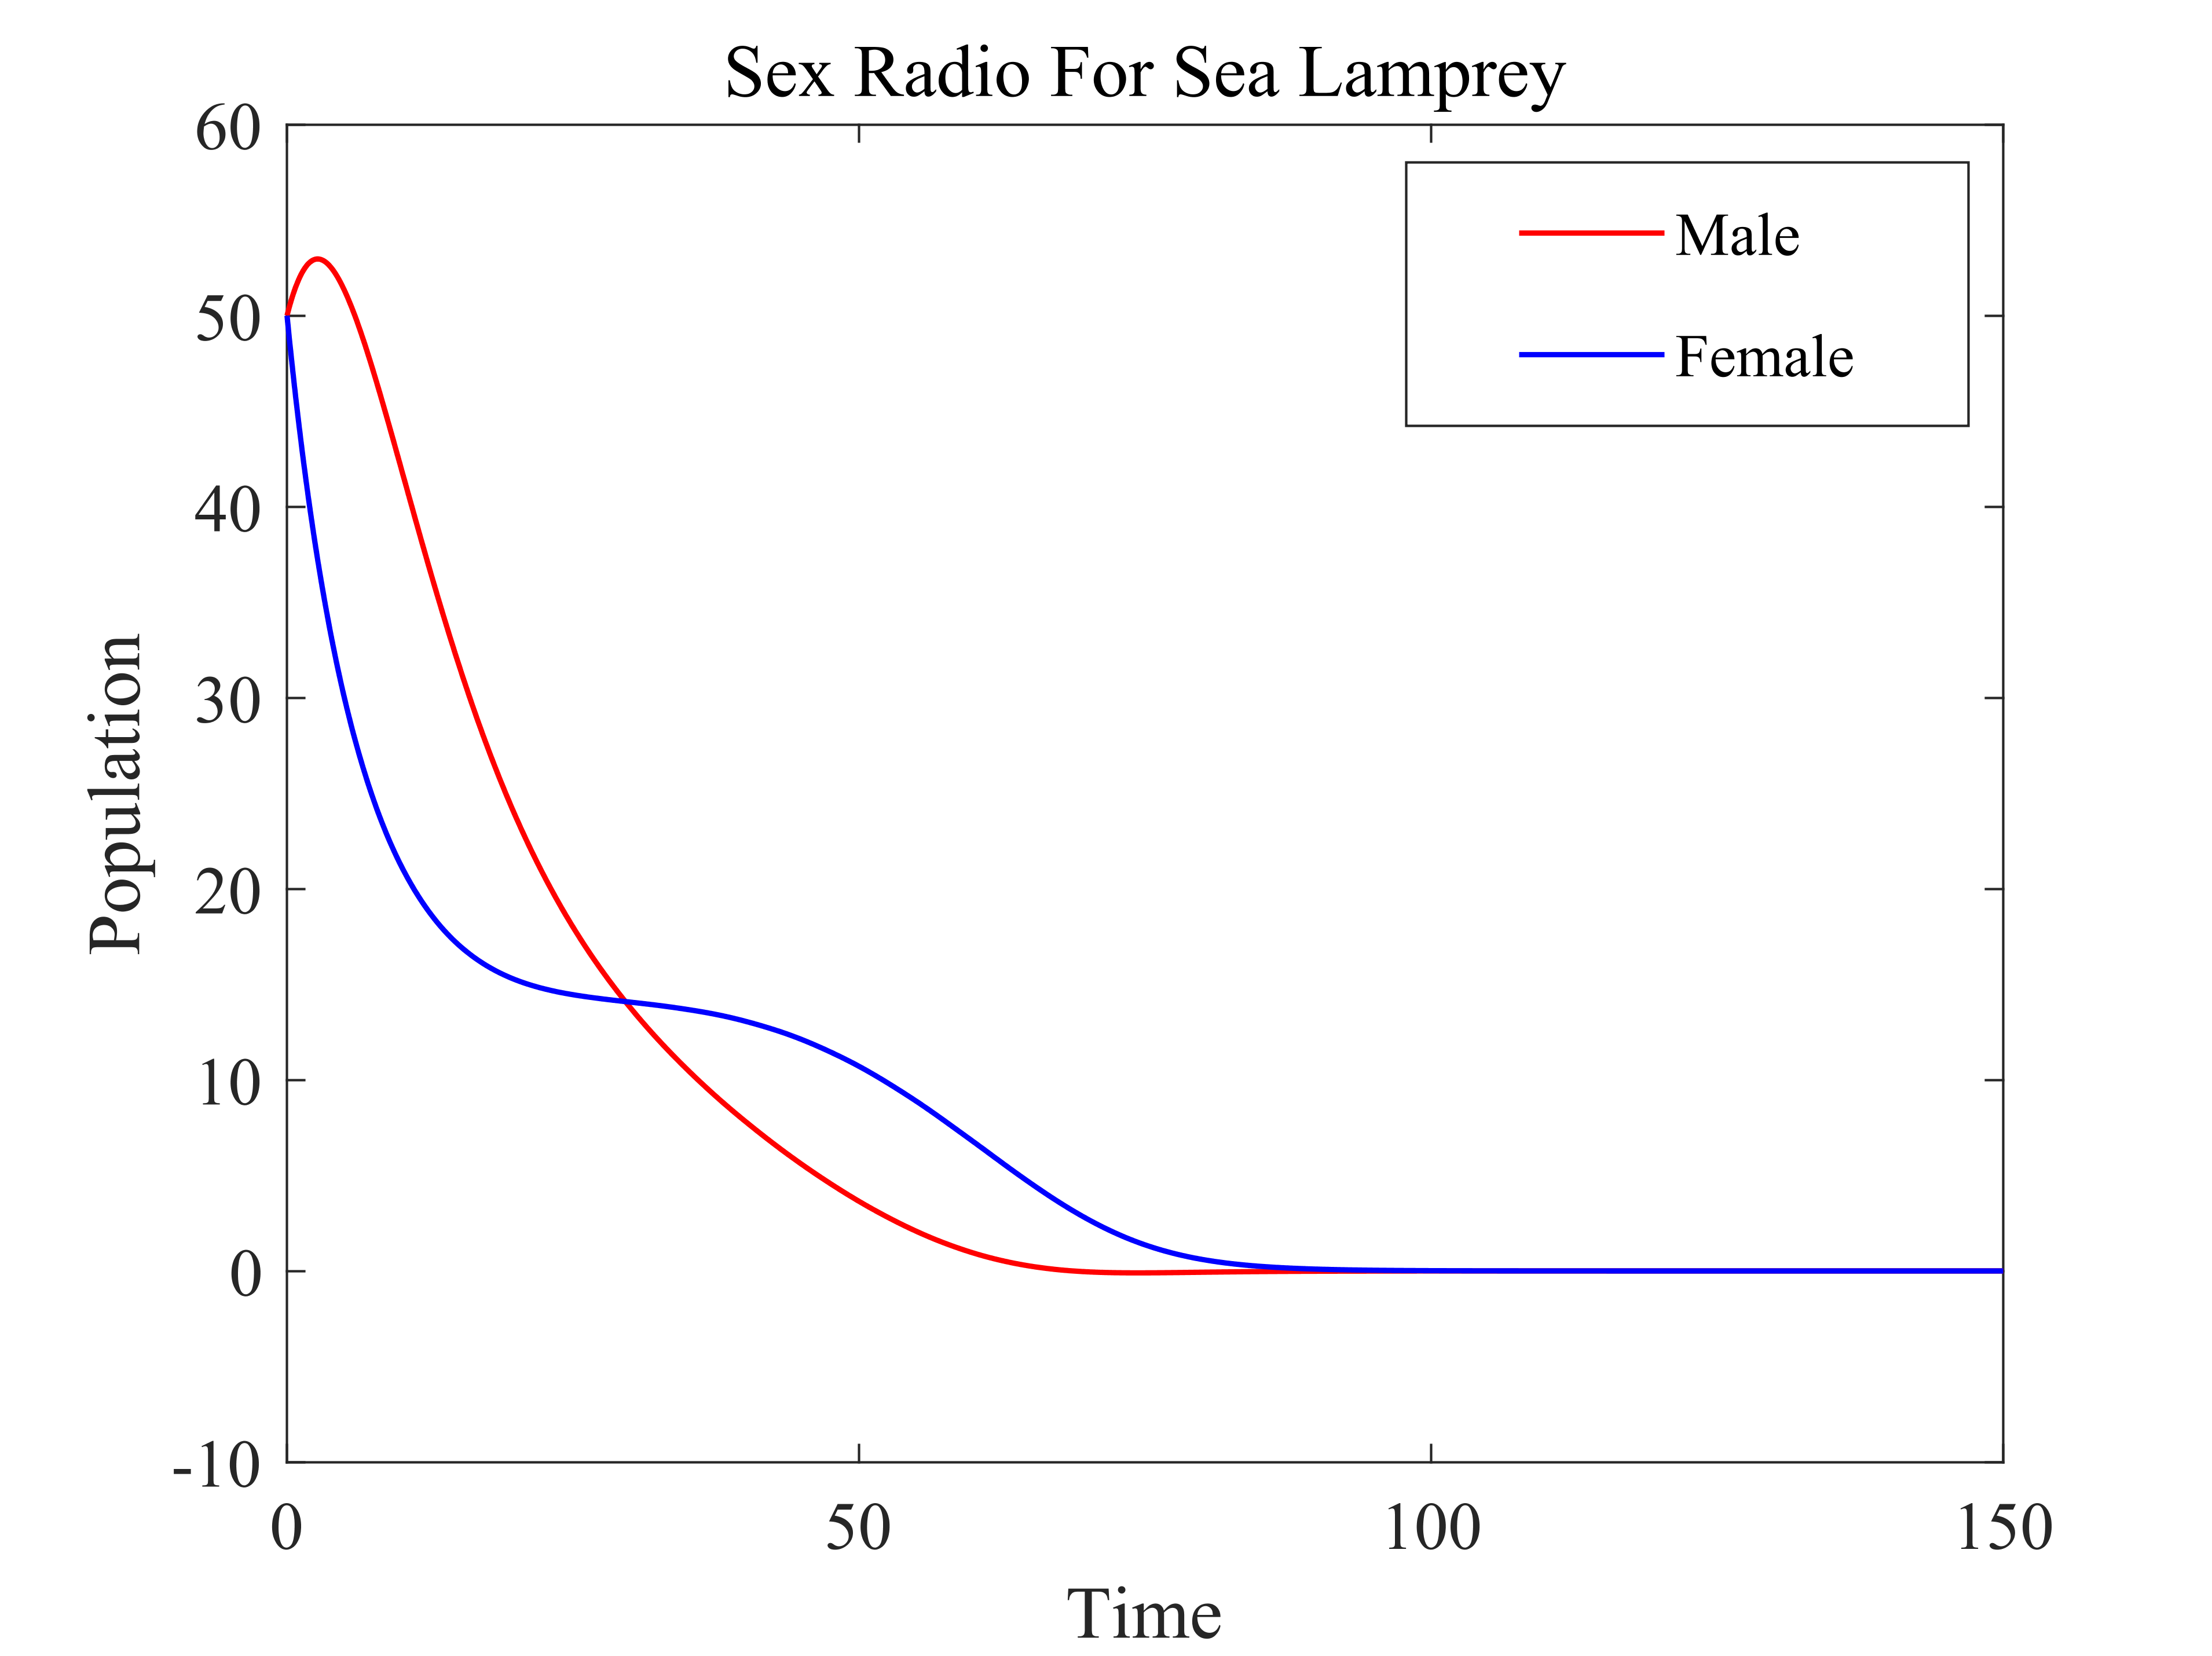
\includegraphics[width=\linewidth]{img/diff21-17071474468901.png}
		\caption{sex diff ratio}
	\end{minipage}
\end{figure}

%在初始食物资源很少的情况下,由图可以看出lamprey的生存能力更差。我们认为原因可能是资源可用性低的环境下lamprey雄性占比高,导致更低的繁殖能力和更高的捕食效率,抑制自身种群的扩张加速自身数量的衰减。
The figure 9, figure 10 make it clear that the lamprey's chances of survival are reduced when there are limited early feeding sources. We think that the reason might be that the high percentage of males in an environment with limited resources causes the lamprey to have a reduced reproductive capability and a higher predation efficiency, which prevents the population from growing and speeds up its own decline.



 %从这两个模型的对比结果中可以得出一些关于对生态系统影响的结论:
 From these three comparison findings, several inferences concerning the influence on ecosystems may be made:\par
 % 物种多样性效应:多样性是衡量生态系统中物种的数量和多样性。多样性的增加可以增加系统的稳定性,减少外部干扰的影响。
 Effect of species diversity: In an ecosystem, diversity refers to the quantity and variety of species present. Increasing variety lessens the effect of outside disruptions and boosts system stability. According to \upcite{4}, in general, a greater diversity should: 
 \begin{enumerate}[\bfseries (1).]
 	\item increase community temporal stability; 
 	\item decrease population temporal stability;
 	\item increase community standing crop and/or productivity;
 	\item decrease amounts of unconsumed limiting resources;
 	\item increase ecosystem stores of limiting nutrients by decreasing loss; 
 	\item decrease invasions by exotic species.
 \end{enumerate}
 %适应性性别比例变化可能带来的优点:
\par
 Possible \textbf{advantages} of adaptive sex ratio changes:\par
% 适应环境变化:当环境条件发生变化时,如食物资源出现明显波动,lampreys可以提高适应性,优化生存。
% 减少种内斗争:使得每个个体更容易获取生存所需的资源,减少生存所需要的资源量,对资源的利用效率提高
%维持种群稳定性和遗传多样性:有助于优化种群动态
\begin{enumerate}[\bfseries (1).]
	\item Adaptation to environmental changes: Lampreys are able to enhance their ability to adapt and maximize their survival in response to changes in their surroundings, such as notable variations in food sources. This may also be the key to their ability to live and procreate for hundreds of millions of years.
	\item Minimizing intraspecific battles means lowering the quantity of resources required for survival and facilitating access to these resources for each individual. Improved effectiveness in the use of available resources.
	\item Preserving genetic variety and population stability: assisting in the long-term development of populations as well as the optimization of population dynamics.
\end{enumerate}


%适应性性别比例变化可能带来的缺点:
% 种群稳定性:过度的适应性性别比例变化可能导致种群的不稳定性,甚至出现种群灭绝或失衡的问题。
% 种群天然平衡不稳定:性别比例明显变化会影响种群天然平衡,雌性占比太少,导致繁殖率陡降,影响稳定
%种群生物量扩大增幅有限,在物种竞争时不具备很强竞争力
Possible \textbf{disadvantages} of adaptive sex ratio changes:
\begin{enumerate}[\bfseries (1).]
	\item Population stability: Population imbalance or even extinction can result from excessive adaptive sex ratio shifts.
	\item Instability of the population's natural balance: notable shifts in the sex ratio have an impact on the population's natural balance. For example, a low number of females causes a sharp drop in reproduction rates, which undermines stability.
	\item Population biomass expansion is limited, and species competition is not very fierce.
\end{enumerate}




\subsection{Expanding the model to include many species}
%在这个部分中,我们构建了一个考虑多物种之间相互作用和资源利用的模型,利用该模型,对物种种群数量随时间变化进行模拟。
In this part, we built a model that considers resource utilization and interactions between many species, which we used to simulate changes in species populations over time.\par
\subsection{Modified logistic modeling}
%首先,我们考虑最理想情况,在无限的空间和其他资源的情况下,物种规模可以无休止的生长
First, we examine the best-case scenario, in which species sizes are infinitely expandable given an infinite amount of room and other resources.\par
\begin{equation}
	\begin{aligned}
		\frac {dN}{dt} &= r \cdot N
	\end{aligned}
\end{equation}
\par
% 实际条件下,环境具有最大承载力,单物种理想种群增长的Logistic模型如下式:
The following equation is the logistic model for the optimum population increase of a single species under real-world circumstances, when the ecosystem has a maximum carrying capacity:\par
\begin{equation}
	\left\{
	\begin{aligned}
		\frac {dx_ {i}}{dt} & = r_ {i}  x_ {i}  (1-  \frac {x_ {i}}{N_ {i}})	\\
		r_i &= \text{birth\_rate} - \text{death\_rate}
	\end{aligned}
	\right.
\end{equation}
\par
${N_ {i}}$ indicates the maximum number of a single species at a particular environmental capacity, $x_ {i} $ indicates the number of a single species i, and $r_i$ indicates the average growth rate of each individual under optimal conditions in the equation above. \par
%食物供应影响幼虫生长速度,进而sea lampreys影响性别比例。在考虑捕食关系时,需要引入校正值,如式
Food availability affects larval growth rate, and in turn sea lampreys affect sex ratio. When considering the predation relationship, it is necessary to introduce a correction value, as in Equation.
\begin{equation}
	\begin{aligned}
		\frac{dx_i}{dt} &= r_i x_i \left(1 - \frac{x_i}{K_i}\right) - \sum_{j \neq i} \alpha_{ij} c_{ij} x_i x_j
	\end{aligned}
\end{equation}
\par
%其中$\alpha_{ij} $表示${x_i}$和${x_j}$之间的捕食强度,$\alpha_{ij} = -\alpha_{ji}$ ,当$\alpha_{ij}$>0时,物种增长速度会因捕食增加。物种多样性是衡量生态系统的重要因素,在考虑种间关系时,需要引入一个校正值$\frac{dx_i}{dt} = r_i x_i \left(1 - \frac{x_i}{K_i} - \sum_{j}\sigma_{ij}\frac{x_j}{K_j}\right) - \sum_{j \neq i} \alpha_{ij} x_i x_j$式中,$\sigma_{ij}$表示$X_i$和$X_j$之间的种间关系指数。当$\sigma_{ij}$<0时,描述互利关系,单一物种数量增长速度会更快。而当$\sigma_{ij}>0$时,种间关系为竞争关系,物种生长率会下降甚至变为负值。
%$c_{ij}$表示捕食者对食物资源的转化率,$c_{ji}$表示被捕食者的被捕食(寄生)的致死率。两个系数共同表示种群的捕食强度。
The intensity of predation between ${x_i}$ and ${x_j}$ is denoted by $\alpha_{ij}$. $\alpha_{ij} = -\alpha_{ji}$. $c_{ij}$ denotes the conversion rate of the predator to the food resource, and $c_{ji}$ denotes the predation (parasitism) lethality of the prey. Together, the two coefficients indicate the predation intensity of the population. And when $\alpha_{ij}$ > 0, predation causes a rise in the rate of species growth. \par
%海七鳃鳗幼体的食性以及成体后的寄生行为使得其更容易携带和传播寄生虫[1],为了刻画这种种间关系,需要引入一个校正值:
Sea lamprey larvae are more prone to carry and spread parasites due to their eating patterns and adult parasitic behavior\upcite{2}.Species diversity is a crucial indicator of ecosystem health, and when taking interspecific connections into account, a correction value must be included.


\begin{equation}
	\begin{aligned}
		\frac{dx_i}{dt} &= r_i x_i \left(1 - \frac{x_i}{K_i} - \sum_{j}\sigma_{ij}\frac{x_j}{K_j}\right) - \sum_{j \neq i} \alpha_{ij} c_{ij} x_i x_j
	\end{aligned}
\end{equation}
\par

where the index of the interspecies link between $X_i$ and $X_j$ is indicated by $\sigma_{ij}$.  A mutualistic connection is described when $\sigma_{ij}$>0, and the population of a single species will expand more quickly. Additionally, the interspecies interaction is competitive when $\sigma_{ij}<0$, and species growth rates will drop or even turn negative.
\par
%我们认为捕食强度与性别比例有关,雄性和雌性表现出不同行为特性,可能影响他们作为捕食者的效率。此外雌性和雄性在捕食中可能对资源利用有不同效率,性别比例变化调整资源利用率以适应不同环境条件,以满足自身发展需要。

We propose that the degree of predation is correlated with the sex ratio and that behavioral differences between male and females may influence the predators' effectiveness. Furthermore, resource usage in predation may differ between males and females, and variations in sex ratios allow individuals to adapt resource utilization to suit their own developmental requirements in response to varying environmental conditions.\par
%物种间捕食强度指数与性别比例S的关系如下式:
The following equation shows the link between the sex ratio S and the index of predation intensity among species:\par
\begin{equation}
	\begin{aligned}
		\alpha_{ij}(s_i, s_j) &= \alpha_0 + \frac{\beta}{1 + e^{-\gamma(s_i - s_j)}}
	\end{aligned}
\end{equation}
\par
%性别比例会影响繁殖,进而影响增长率。sea lampreys产卵后成虫会死亡。性别比例与增长率的关系如下式:
Growth rate and reproduction are impacted by the sex ratio. After depositing eggs, mature sea lampreys perish. The following equation shows the link between the sex ratio and growth rate:\par
\begin{equation}
	\begin{aligned}
	S(R,A) &= \alpha R(1-R)
	\end{aligned}
\end{equation}
%S表示繁殖成功率,$\alpha$是系数,食物资源量A和猎物与捕食者的数量比例有关
\par
S denotes the reproductive success rate and $\alpha$ is the coefficient. The amount of food resource A is related to the ratio of prey to predator numbers. It is assumed that all non-producer populations are driven by predation and therefore have a constant natural growth rate < 0. 
\begin{equation}
	\begin{aligned}
		A&=\frac{P}{\sum Y_j}
	\end{aligned}
\end{equation}
%对于某个物种 $X_i$ 而言,P表示所有食物的数量,$Y_j$ 表示与 $X_i$ 竞争食物的物种数量(包括 $X_i$ 的数量)
\par
For a given species $X_i$, P denotes the amount of all food, and $Y_j$ denotes the number of species competing with $X_i$ for food (including the number of $X_i$)
%假设所有非生产者的种群增长动力都来自于捕食,因此其自然增长率恒定<0.基于上述分析,可以得到描述物种数量以及相互作用的微分方程,并成功构建数学模型。
\par
The aforementioned analysis may be used to create differential equations that describe the number of species and their interactions, as well as to effectively design mathematical models.
\par
\subsubsection{Quantitative prediction using adjusted models}
%为了定性探究对生态系统的影响,我们模拟了同时包含寄生虫,竞争者和生产者种群的生态系统的演化。分别考虑lamprey的雄性和雌性数量变化。然后我们观察这个生态系统中物种的生物量变化,为了使模拟出更有代表性的长期变化,我们将模拟时间设置较长,结果如下图所示。
We simulated the evolution of ecosystems including producer, competitor, and parasite populations in order to investigate the impacts on ecosystems qualitatively. Changes in the quantity of male and female lamprey were taken into consideration independently. After then, we looked at how the species' biomass changed in this environment. We extended the simulation period to make the model more reflective of long-term changes, and the outcomes are displayed below.
\par
%竞争者1是和lamprey不同的物种,它们相互争夺食物资源
Competitor 1 is a different species than lamprey and they compete with each other for food resources.\par
%竞争者2是和lamprey完全相同的物种,除适应性性别比例变化外
The only difference between competitor 2 and lamprey is the adaptive sex ratio.\par
%通过控制变量对问题进行研究分析,建立包含lamprey或竞争者2的模型,并进行对比,如下图:
The problem was studied and analyzed by controlling the variables to create a model that included lamprey or competitor 2 and compared as follows:
\par
 Changes to ecosystems with parasites, rivals, lamprey, and producers:\par
\begin{figure}[htbp]
	\begin{minipage}[b]{0.5\linewidth}
		\centering
		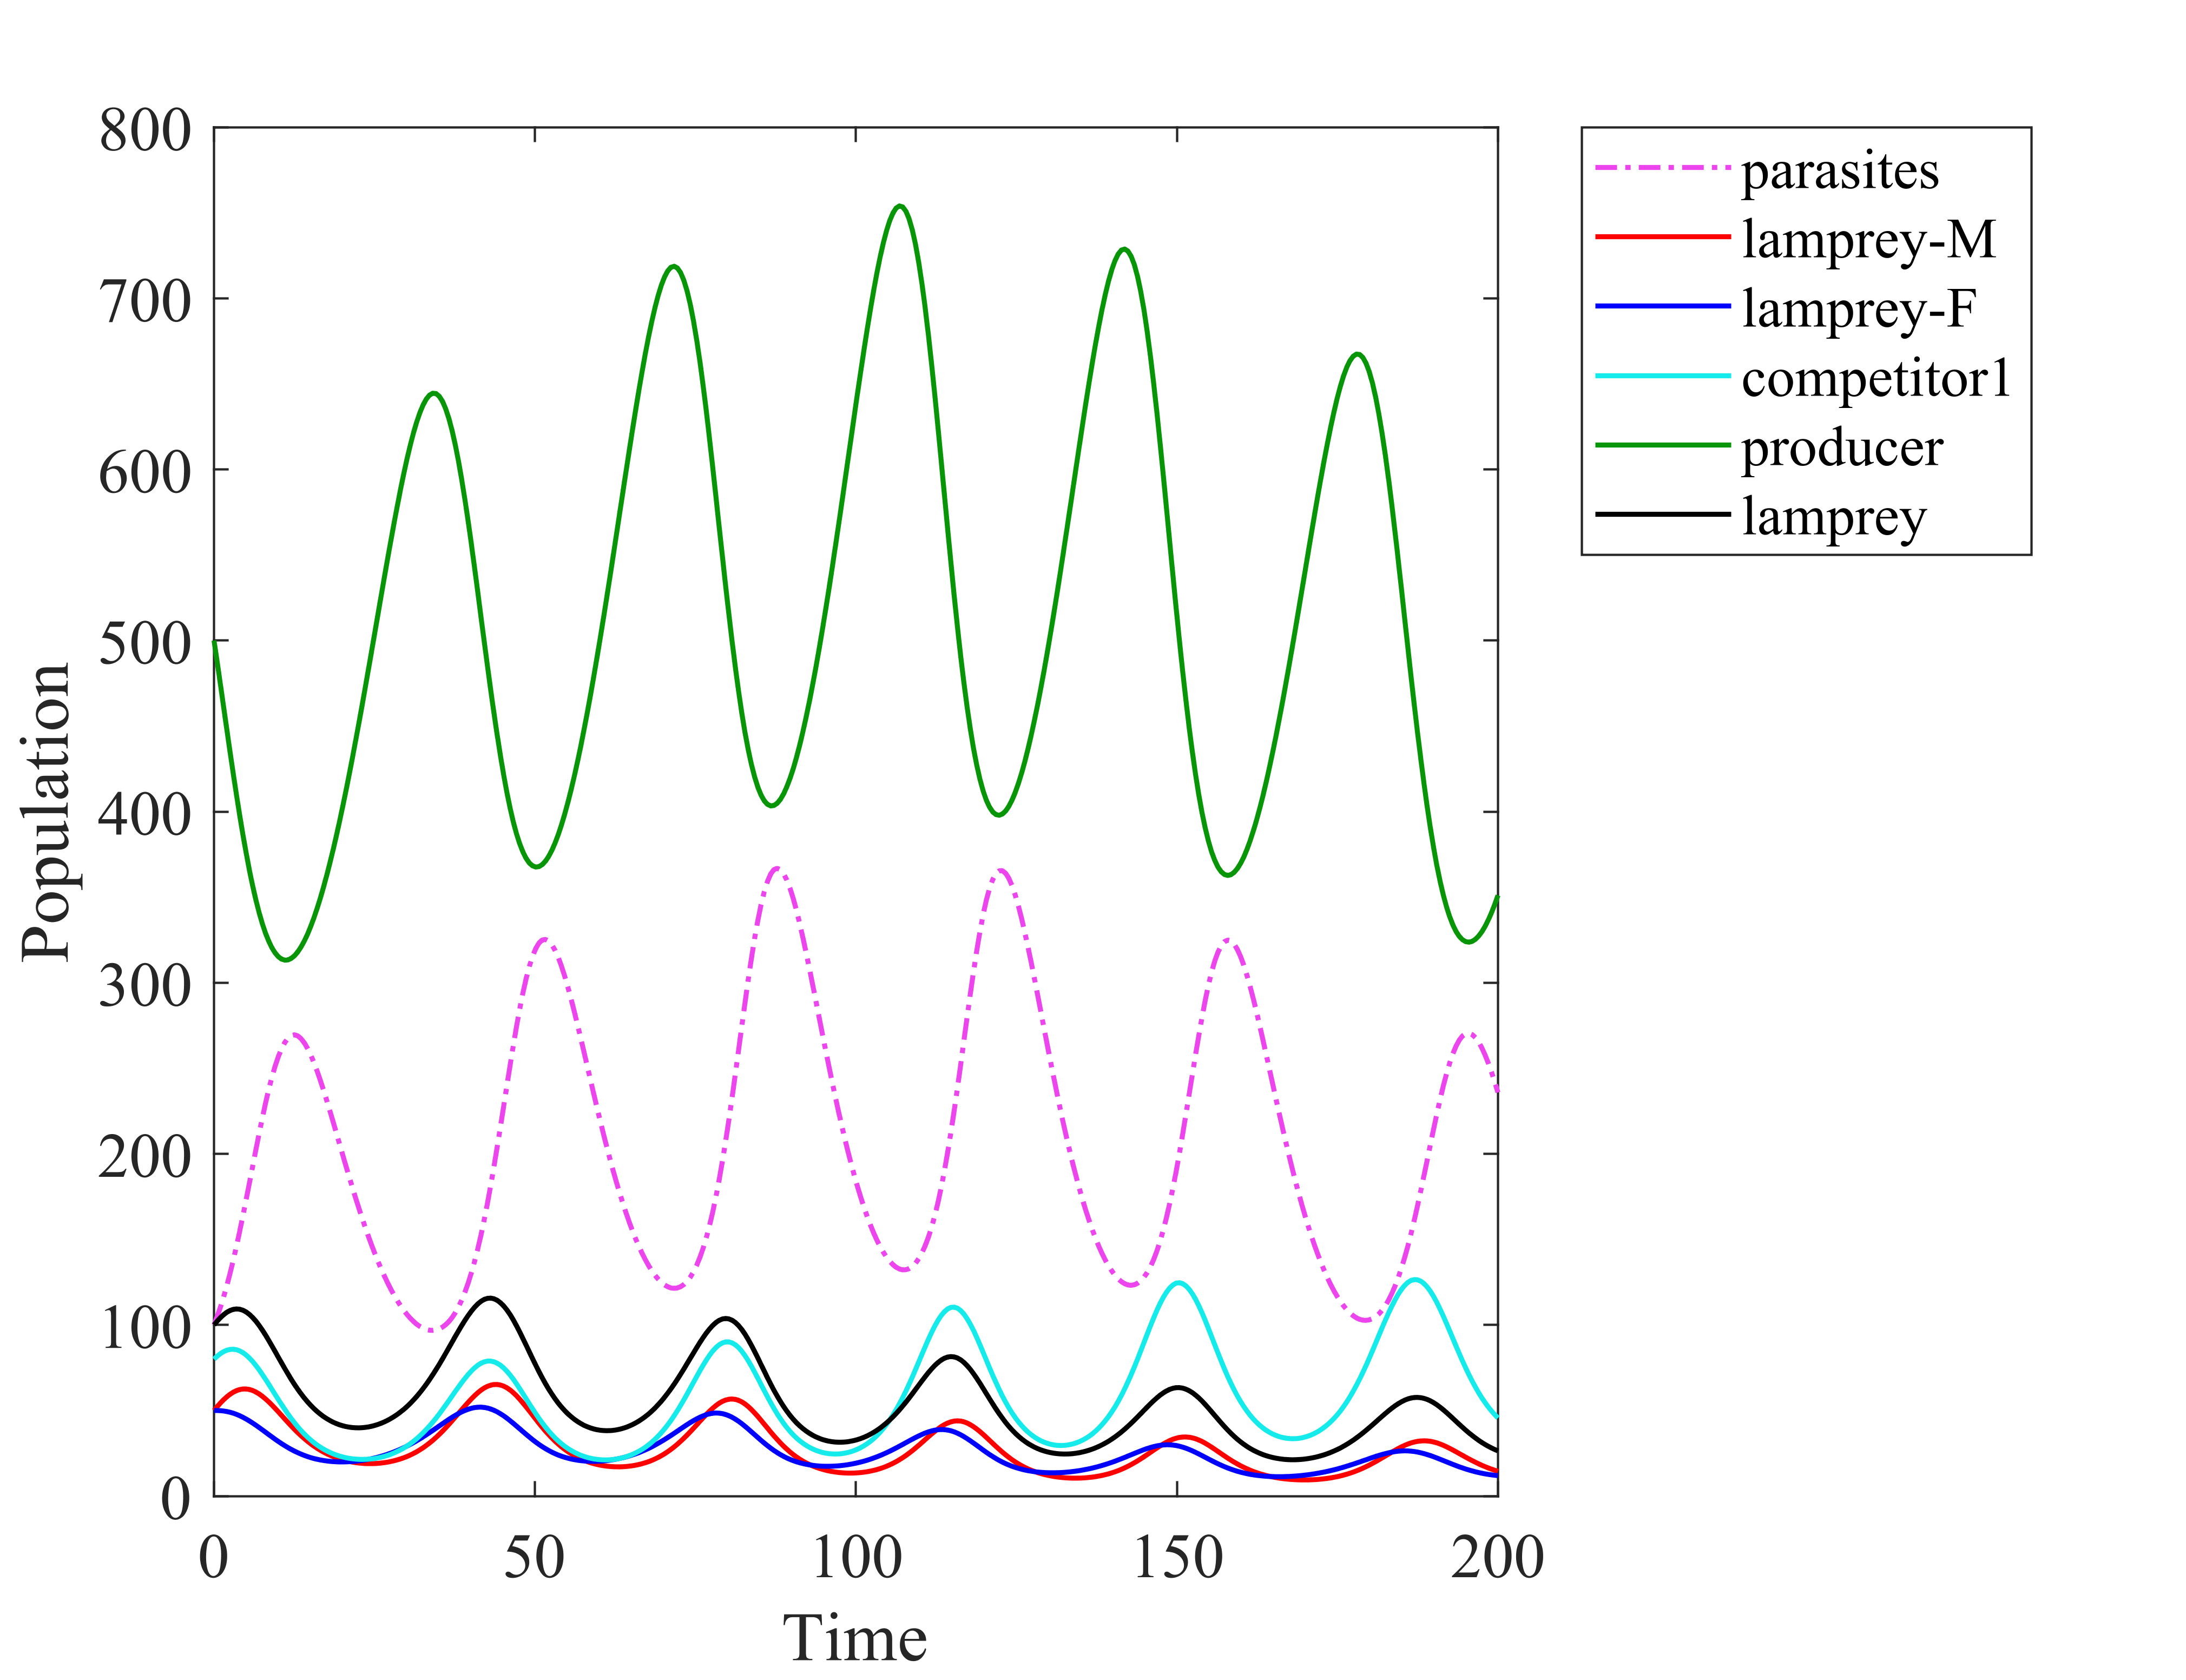
\includegraphics[width=\linewidth]{img/five.png}
		\caption{Short-term}
	\end{minipage}%
	\begin{minipage}[b]{0.5\linewidth}
		\centering
		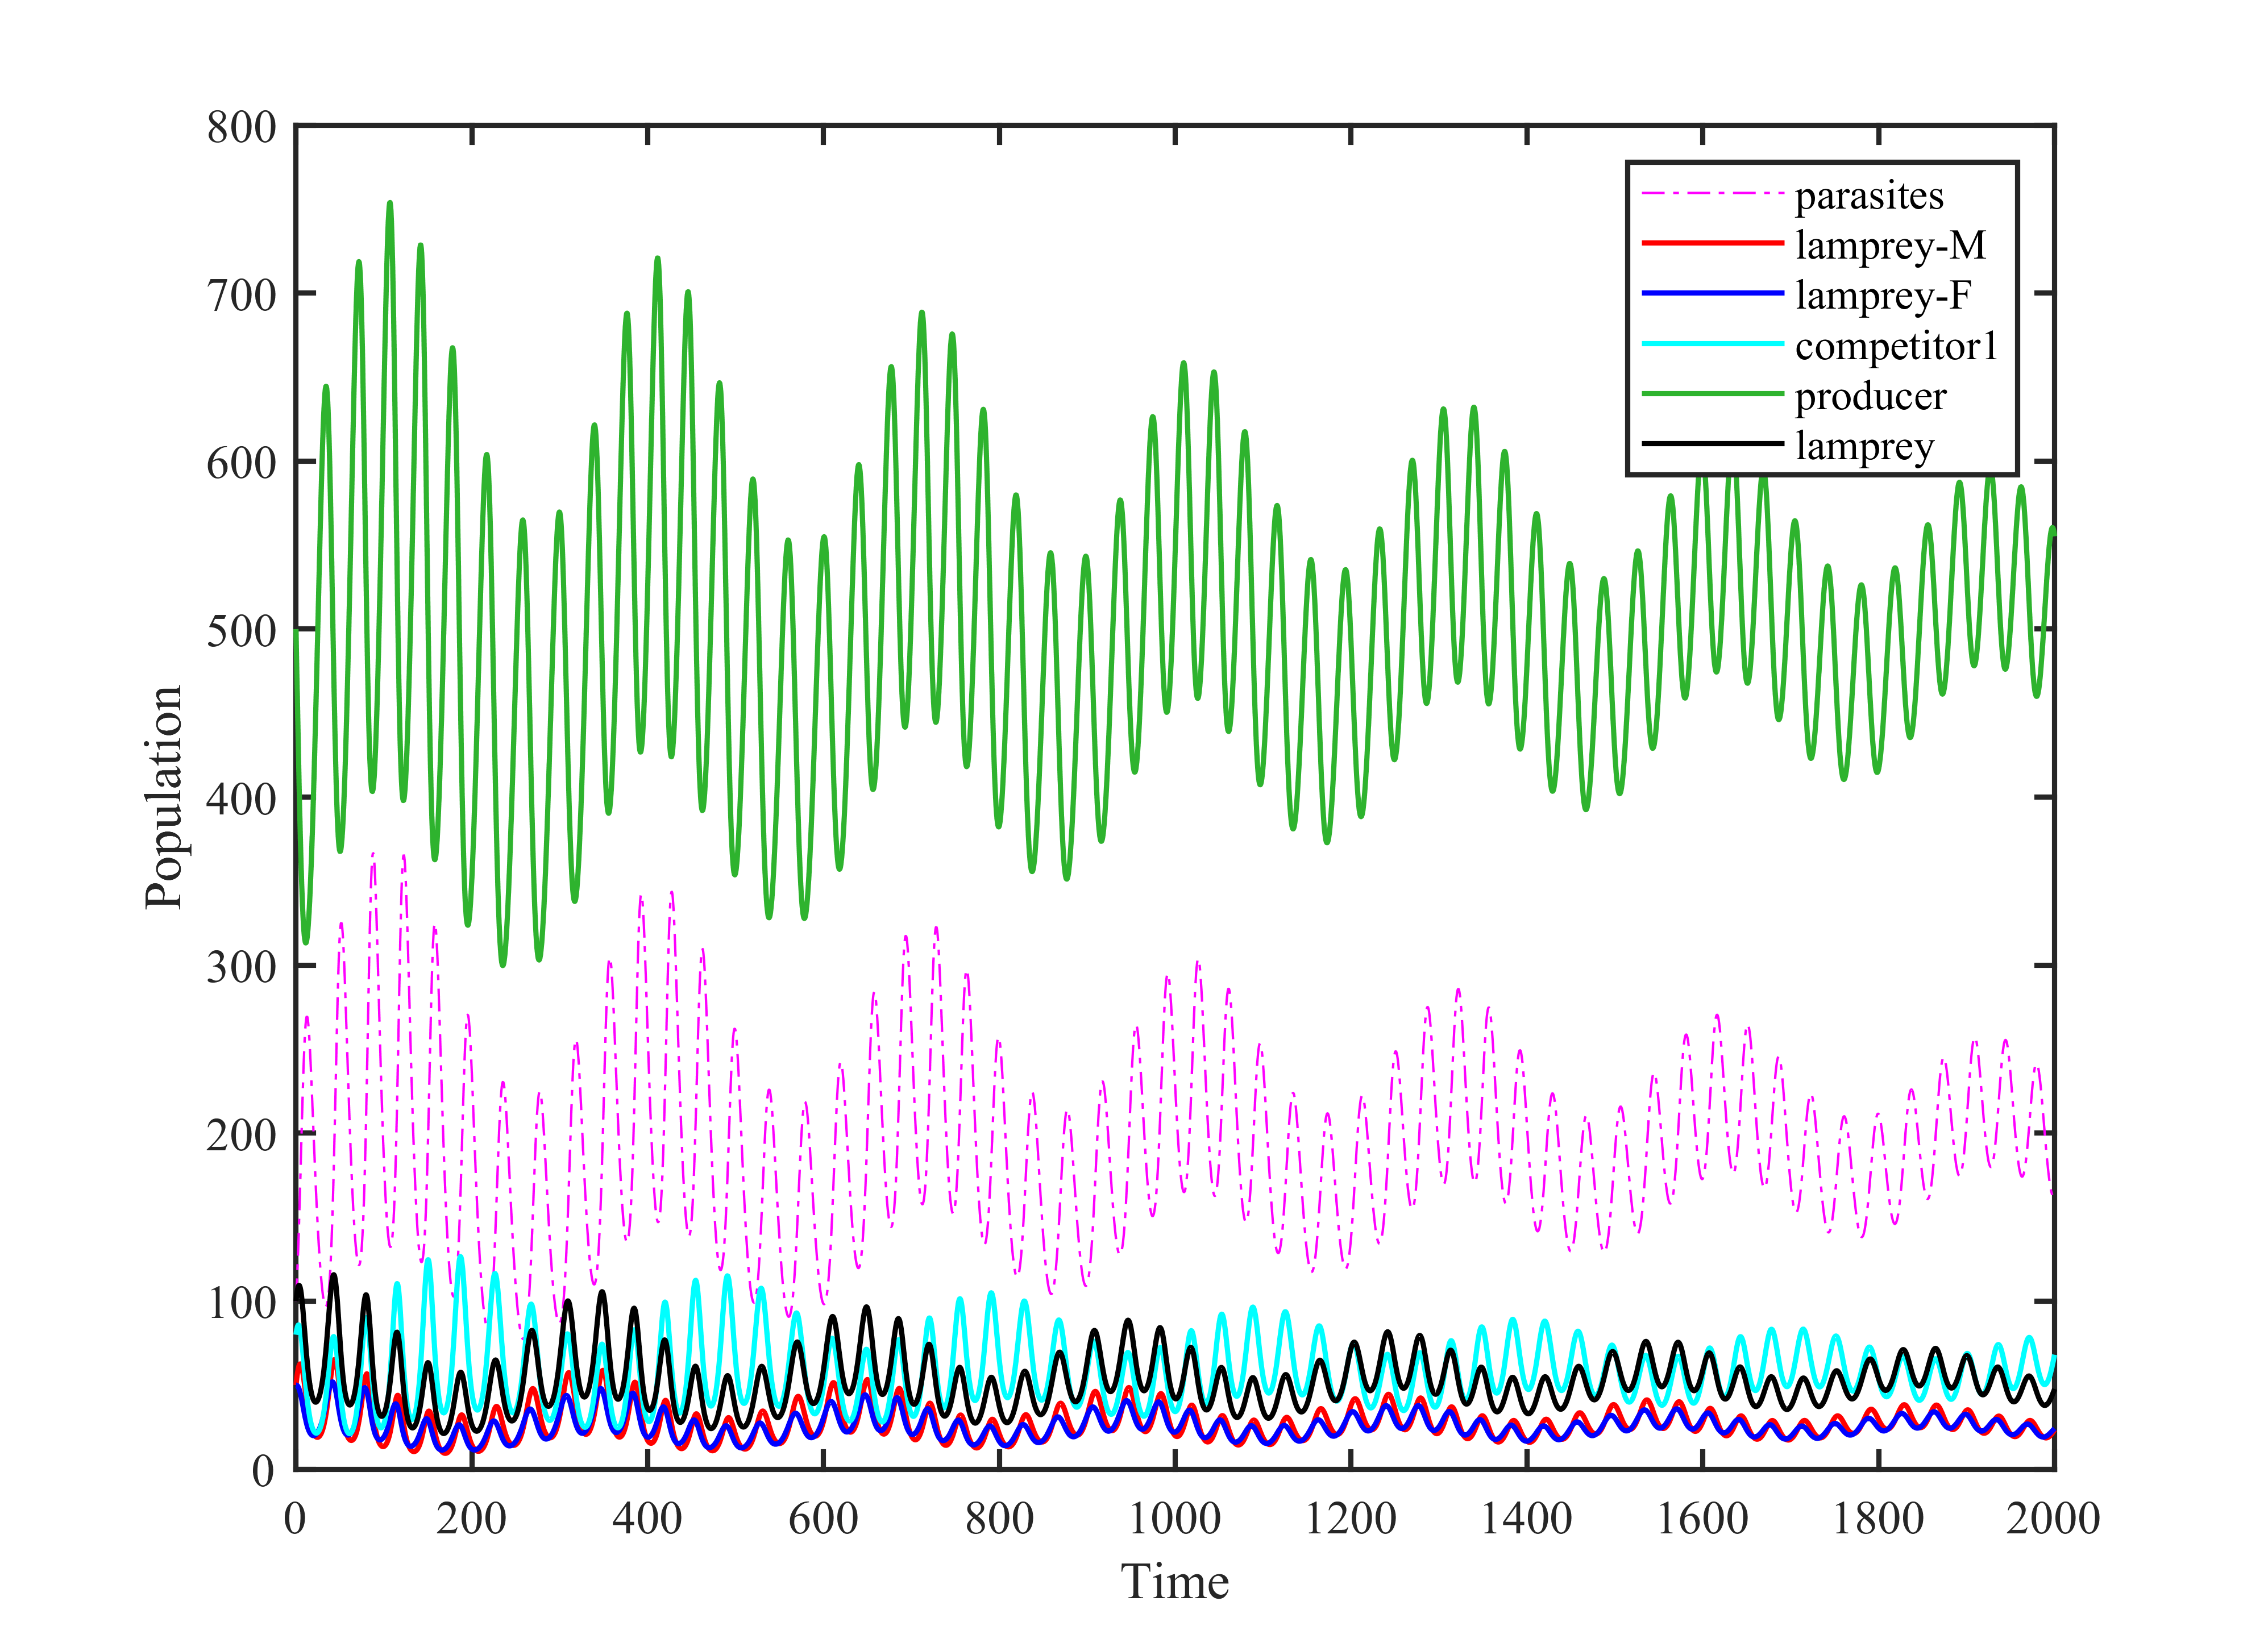
\includegraphics[width=\linewidth]{img/lamprey-17071240598592.png}
		\caption{Long-term}
	\end{minipage}
\end{figure}
 Changes to ecosystems with parasites, rivals, and producers(without lamprey:
\begin{figure}[htbp]
	\begin{minipage}[b]{0.5\linewidth}
		\centering
		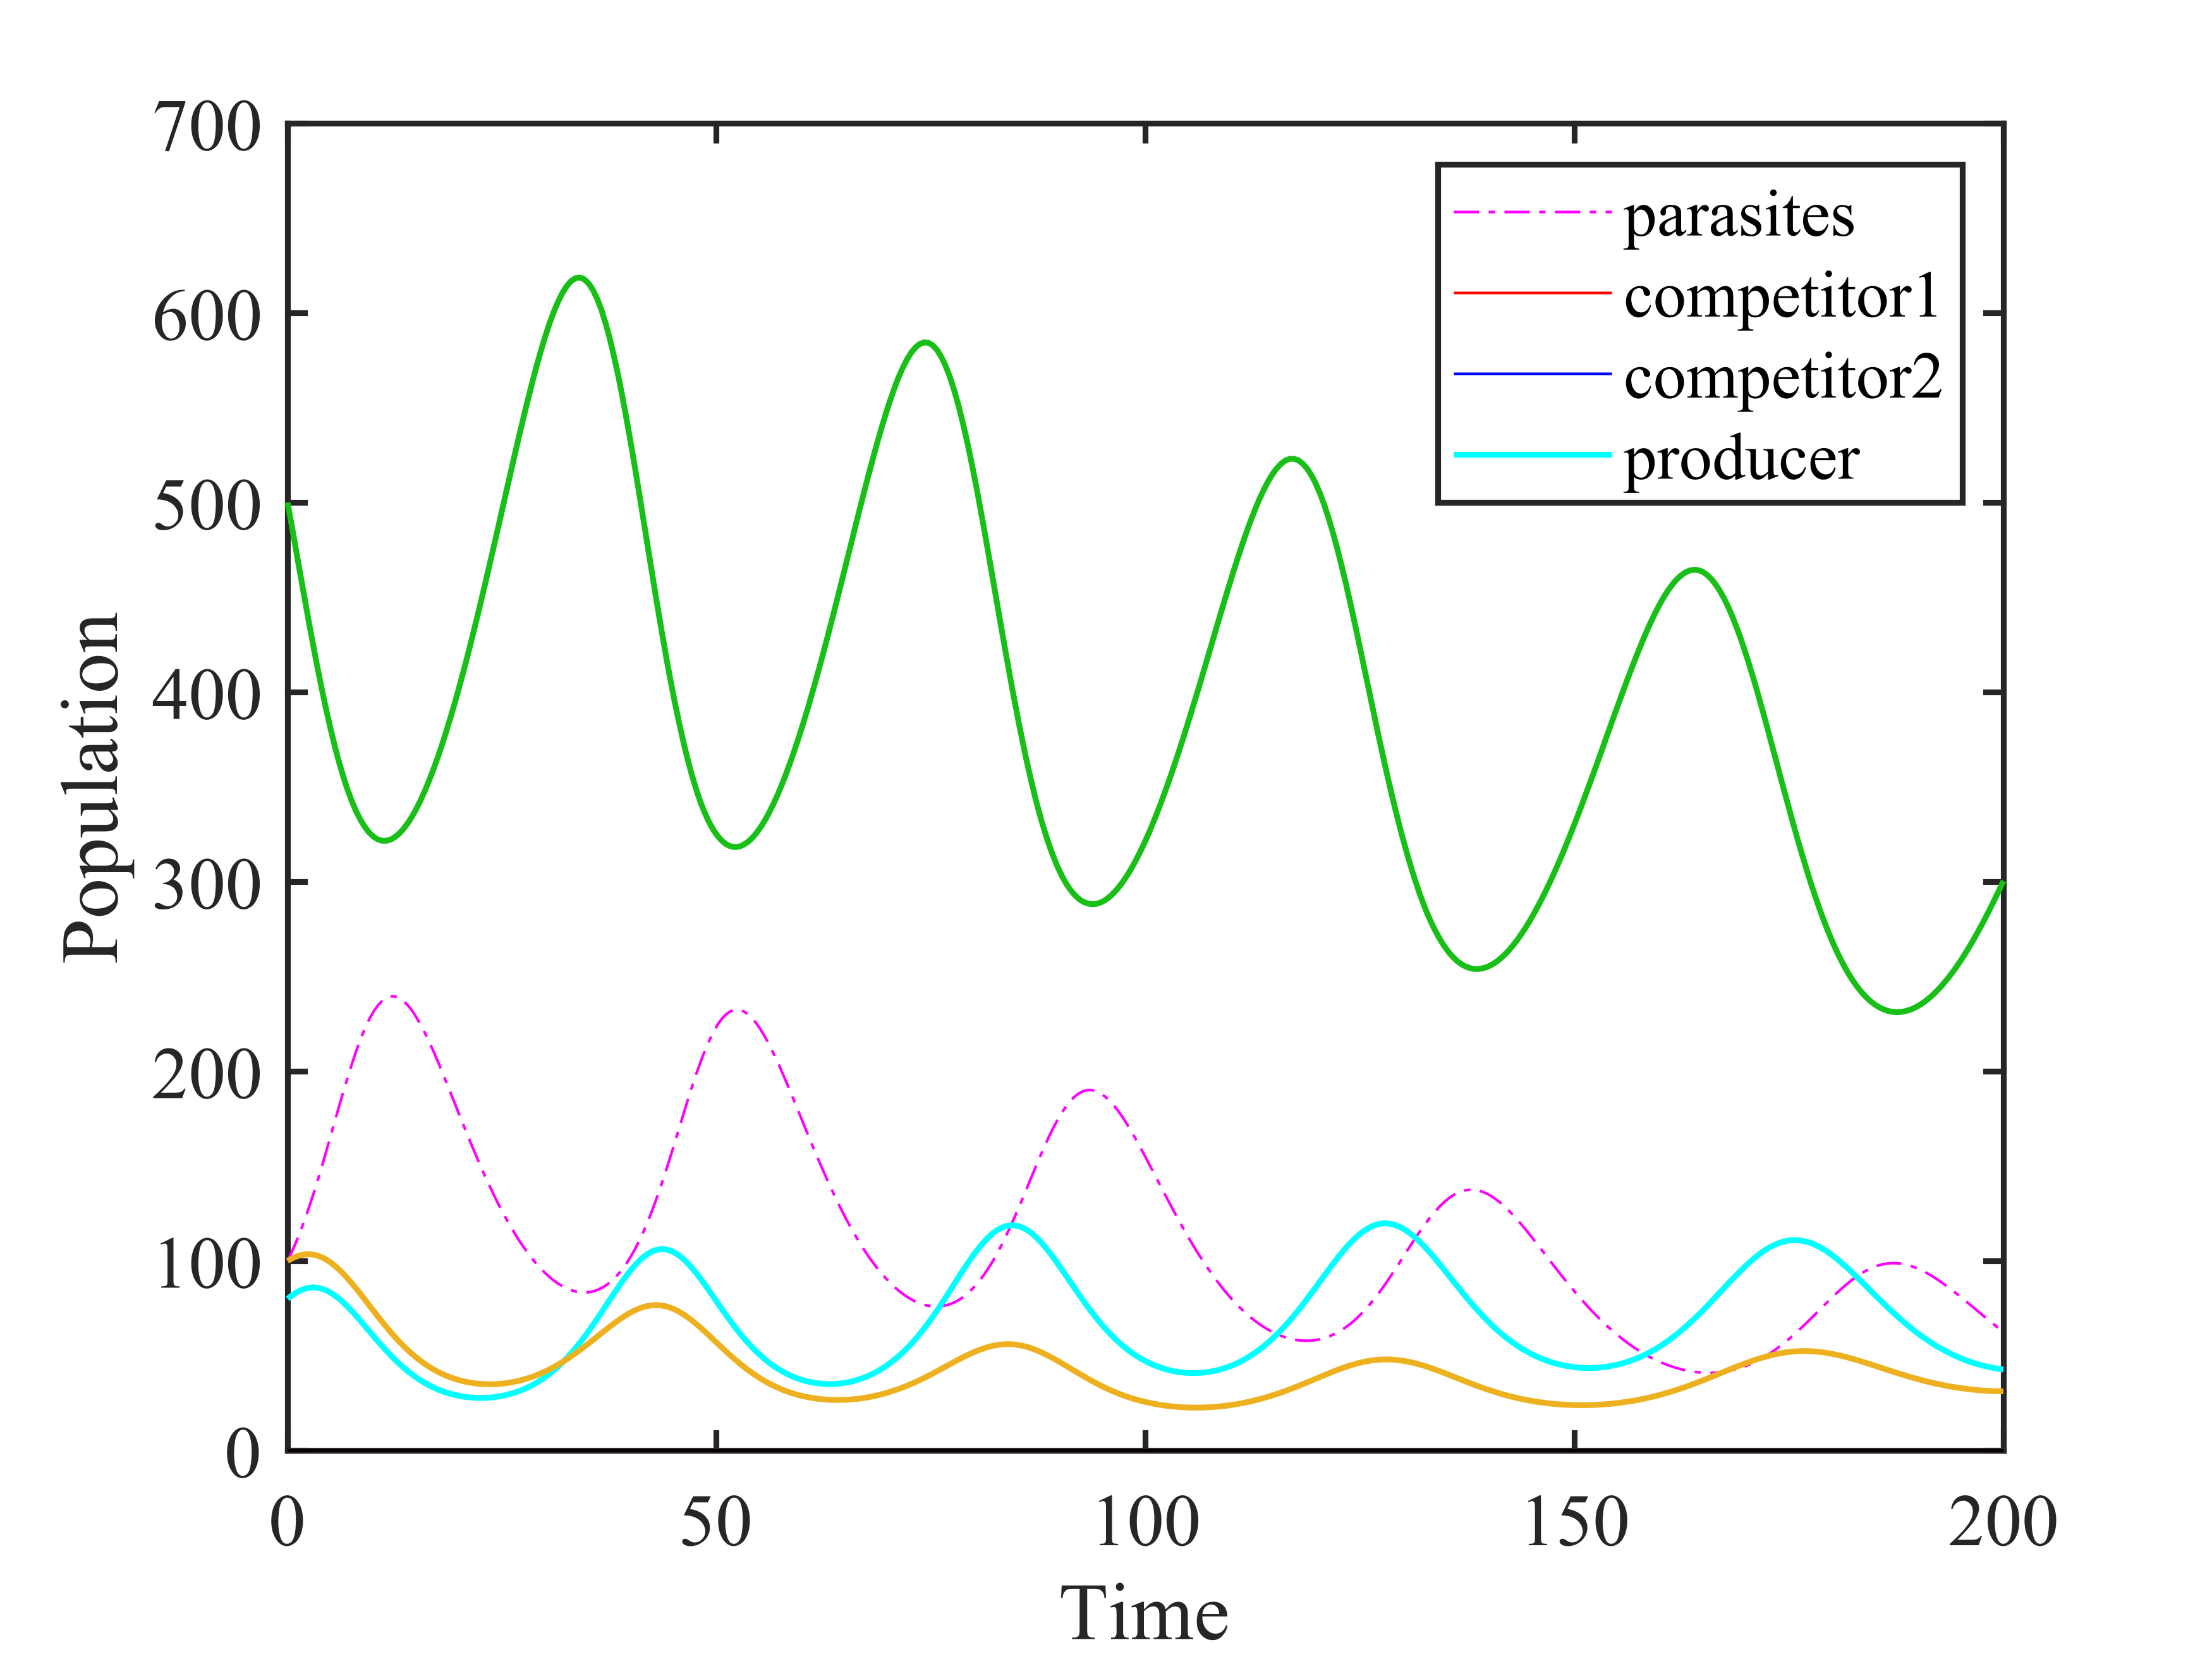
\includegraphics[width=\linewidth]{img/competitor2.png}
		\caption{Short-term}
	\end{minipage}%
	\begin{minipage}[b]{0.5\linewidth}
		\centering
		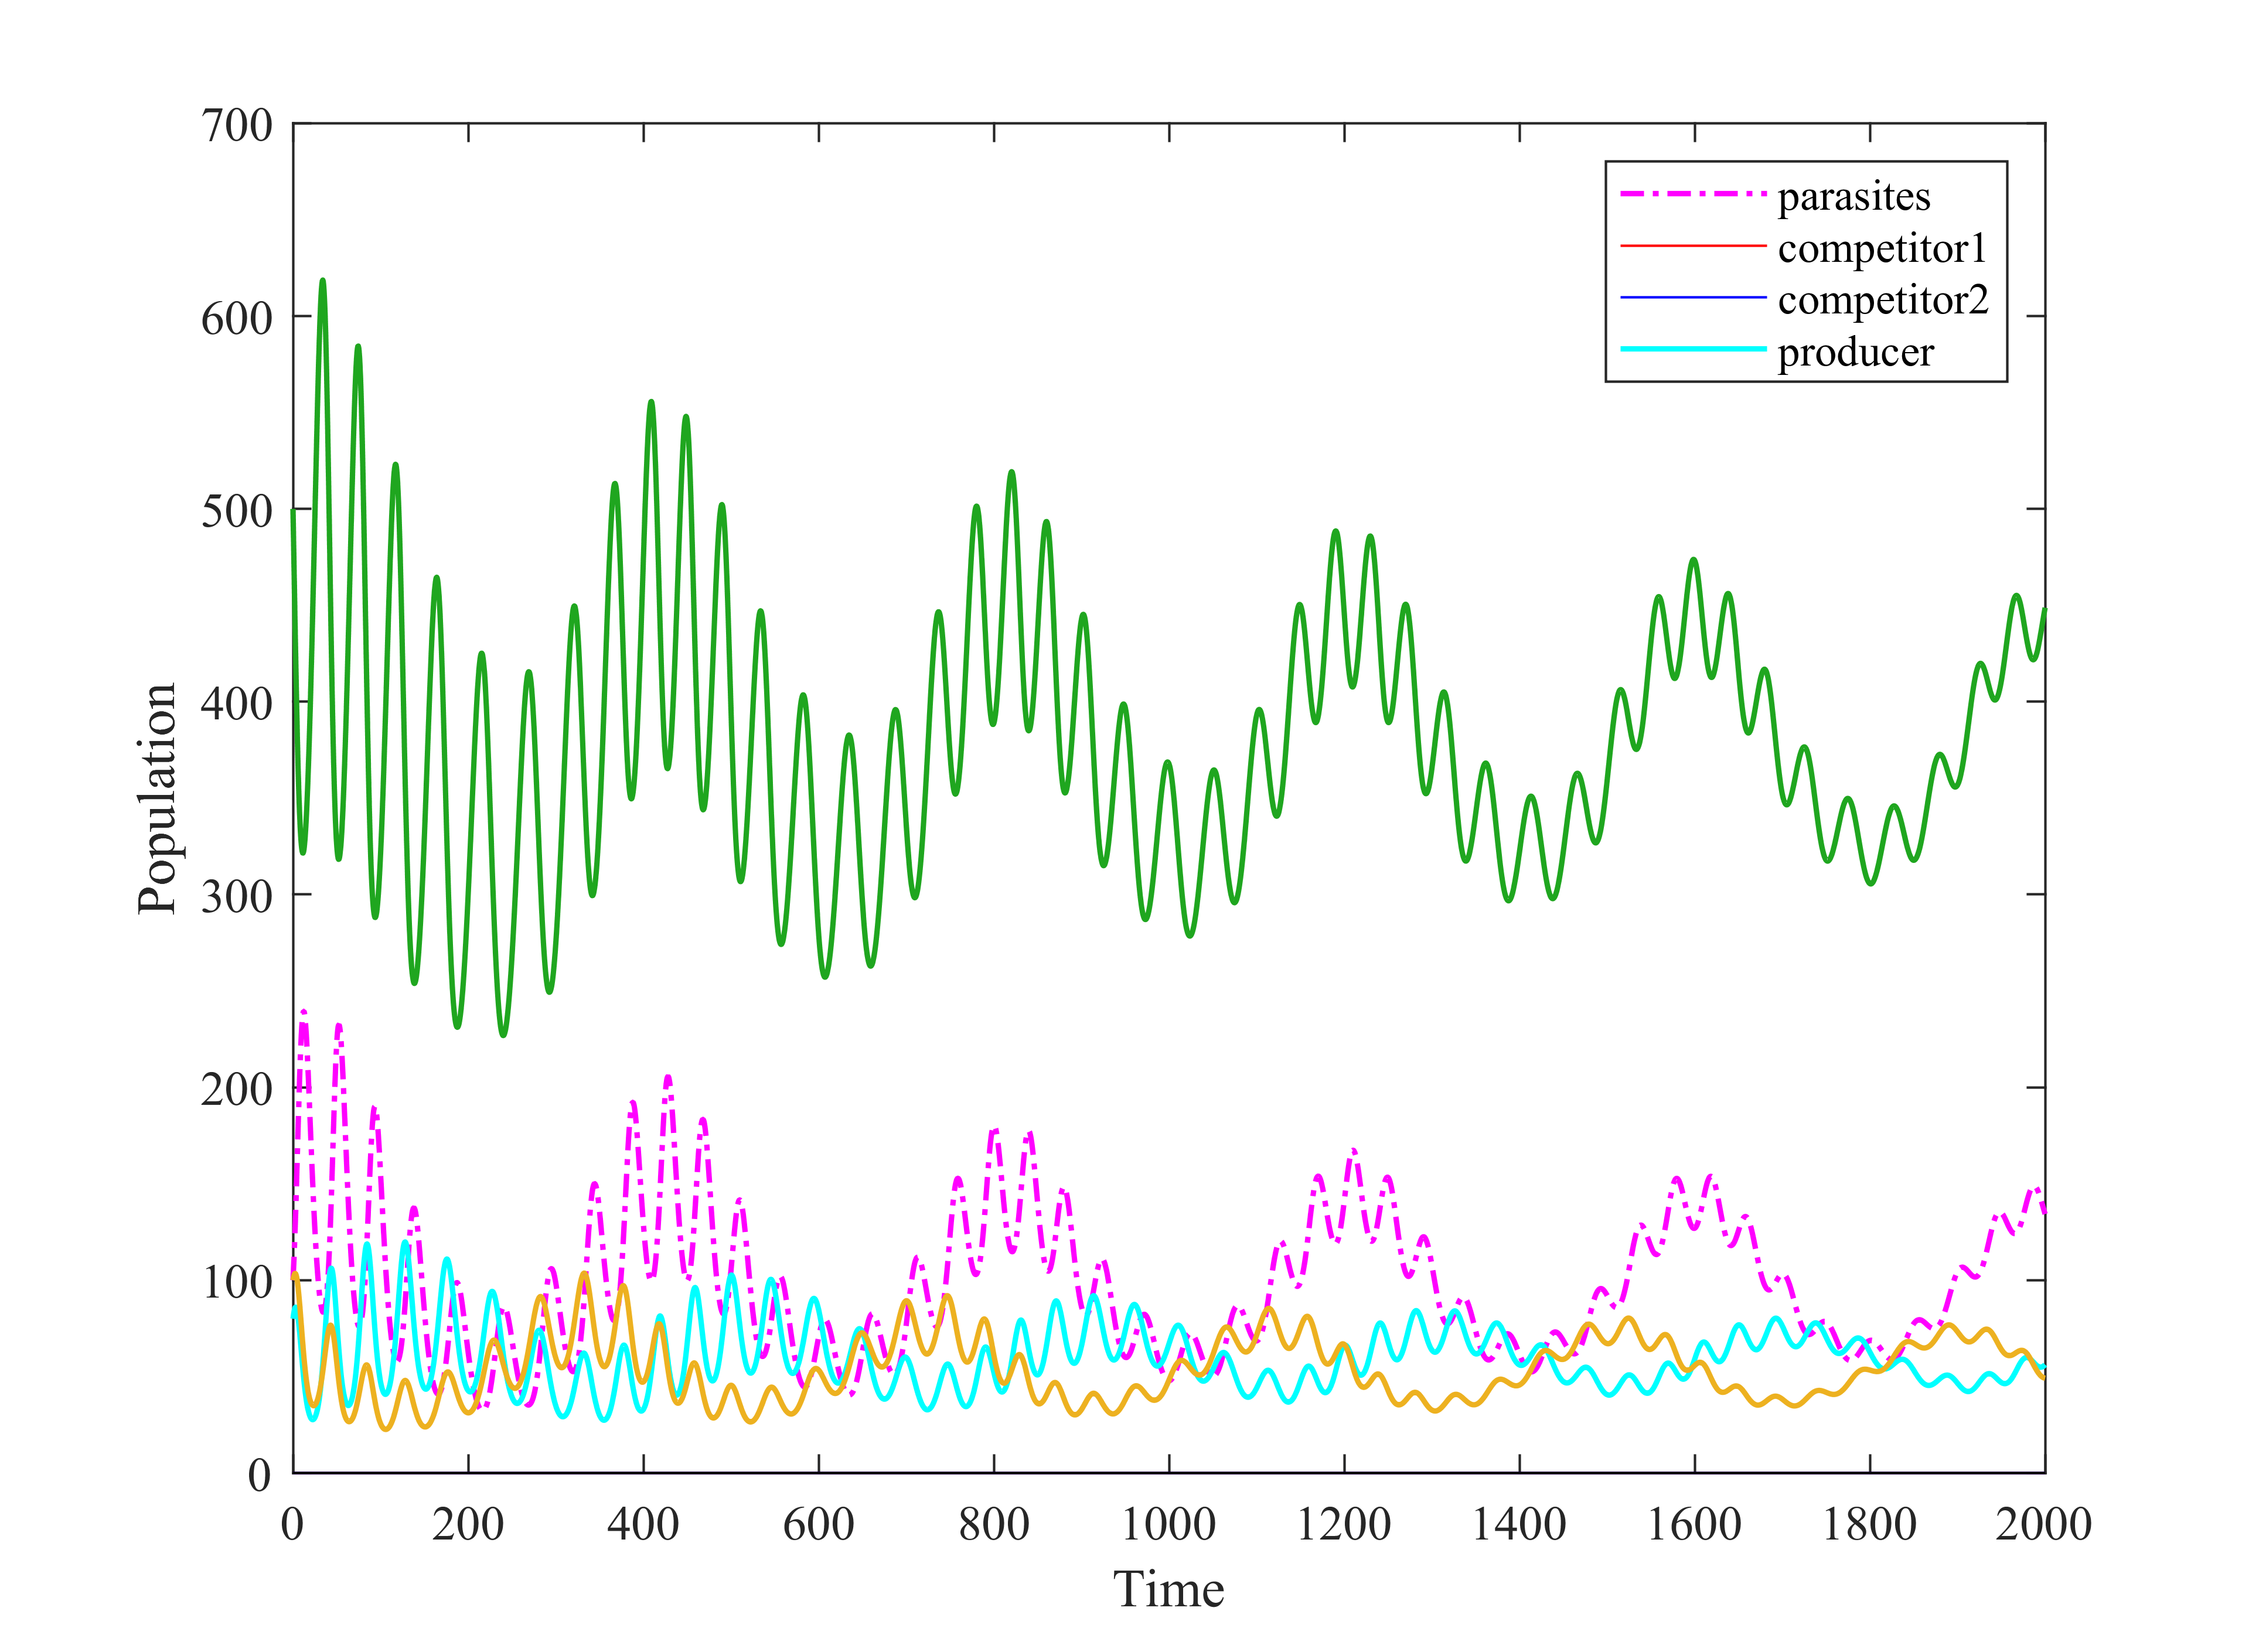
\includegraphics[width=\linewidth]{img/competitor-17071240898223.png}
		\caption{Long-term}
	\end{minipage}
\end{figure}

%从上述图表的对比可以得到一些结论:
\par
Some conclusions can be drawn from the comparison of the above figures:
%lampreys随环境发生的性别比例变化会造成更频繁的生物量波动

%lampreys和竞争者1的生物量变化关系呈现此消彼长的相反方向。这是由于物种之间对于食物和其他资源的竞争对彼此种群增长具有抑制作用

%生态系统中物种的总生物量低于单个物种培养时的总生物量,这是由于增加了物种间相互关系的影响,除了考虑捕食之外。

\begin{enumerate}[\bfseries (1).]
	\item Changes in the sex ratio of lampreys in response to their environment result in more frequent biomass fluctuations.
	\item The variations in biomass in lampreys and competitor 1 exhibit an inverse relationship.This is due to the fact that competition between species for food and other resources has a dampening effect on the growth of each other's populations.
	\item Because of the increasing interrelationships between species, the overall biomass of species in an ecosystem is smaller than the total biomass of individual species in culture. Consider more than just predatory relationships.
\end{enumerate}
\par
%物种之间的种间关系会造成生物量波动。根据物种多样性效应物种共存时总生物量波动较小,表明具有多个物种的生态系统具有更大的稳定性。
Variations in biomass might result from interactions between species that are interspecific. According to the species diversity effect, total biomass swings less when species coexist, suggesting higher stability in ecosystems with diverse species.\par
%为了验证生态系统的稳定性实际上受益于性别比例变化的lamprey和其他物种共存,我们应该定量描述其特征。我们将使用几个具有代表性且易于计算的指标来评估生态系统。
We should quantitatively quantify the presence of lamprey and other species with varying sex ratios to confirm that it truly contributes to the stability of the ecosystem. We want to evaluate the ecosystems using a number of representative and readily computed measures.\par
%生态系统最重要的指标是总生物量,它反映了生态系统中各物种种群的生长状况,若第$i$个物种的生物量记为$x_i$,则该群落的总生物量$TB$ 为所有物种的生物量之和。
The overall biomass of an ecosystem, which reflects the growth condition of the populations of each species inside it, is its most significant indicator. The biomass of all species added together is the total biomass of the community, $TB$, if the biomass of the $i$th species is represented by $x_i$.\par

\begin{figure}[htbp]
	\begin{minipage}[b]{0.5\linewidth}
		\centering
		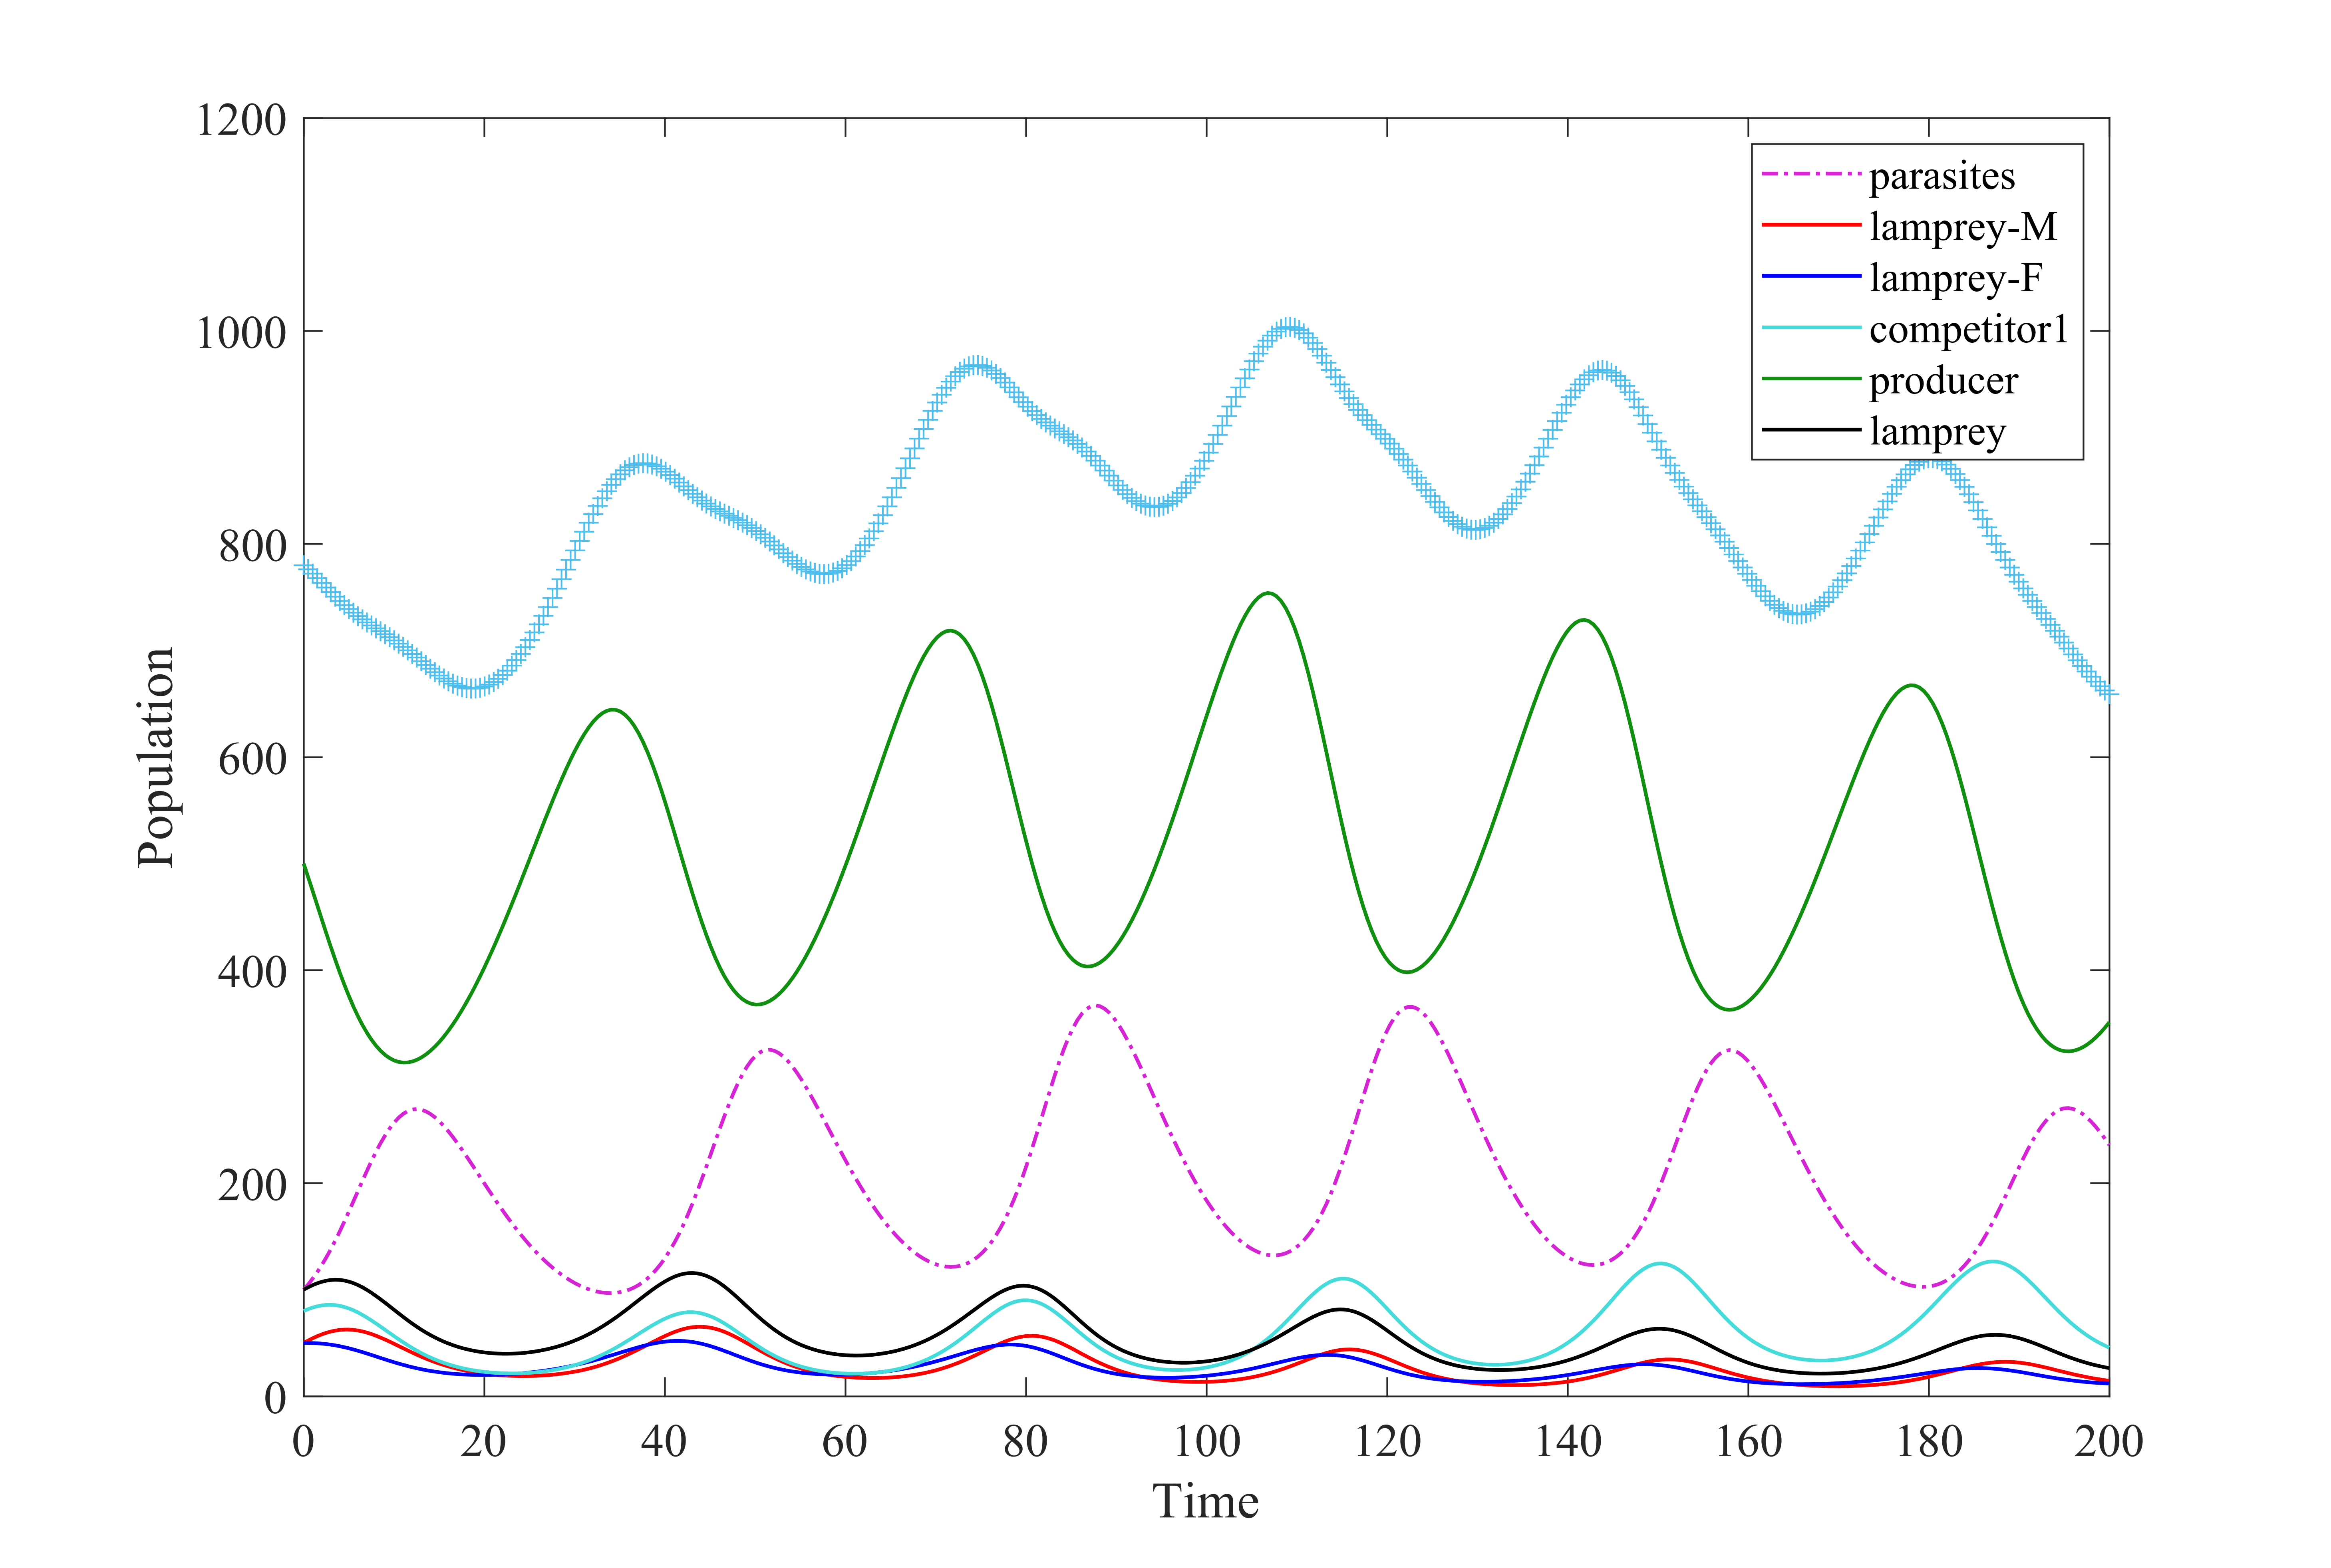
\includegraphics[width=\linewidth]{img/sum.png}
		\caption{Sum 1 }
	\end{minipage}%
	\begin{minipage}[b]{0.5\linewidth}
		\centering
		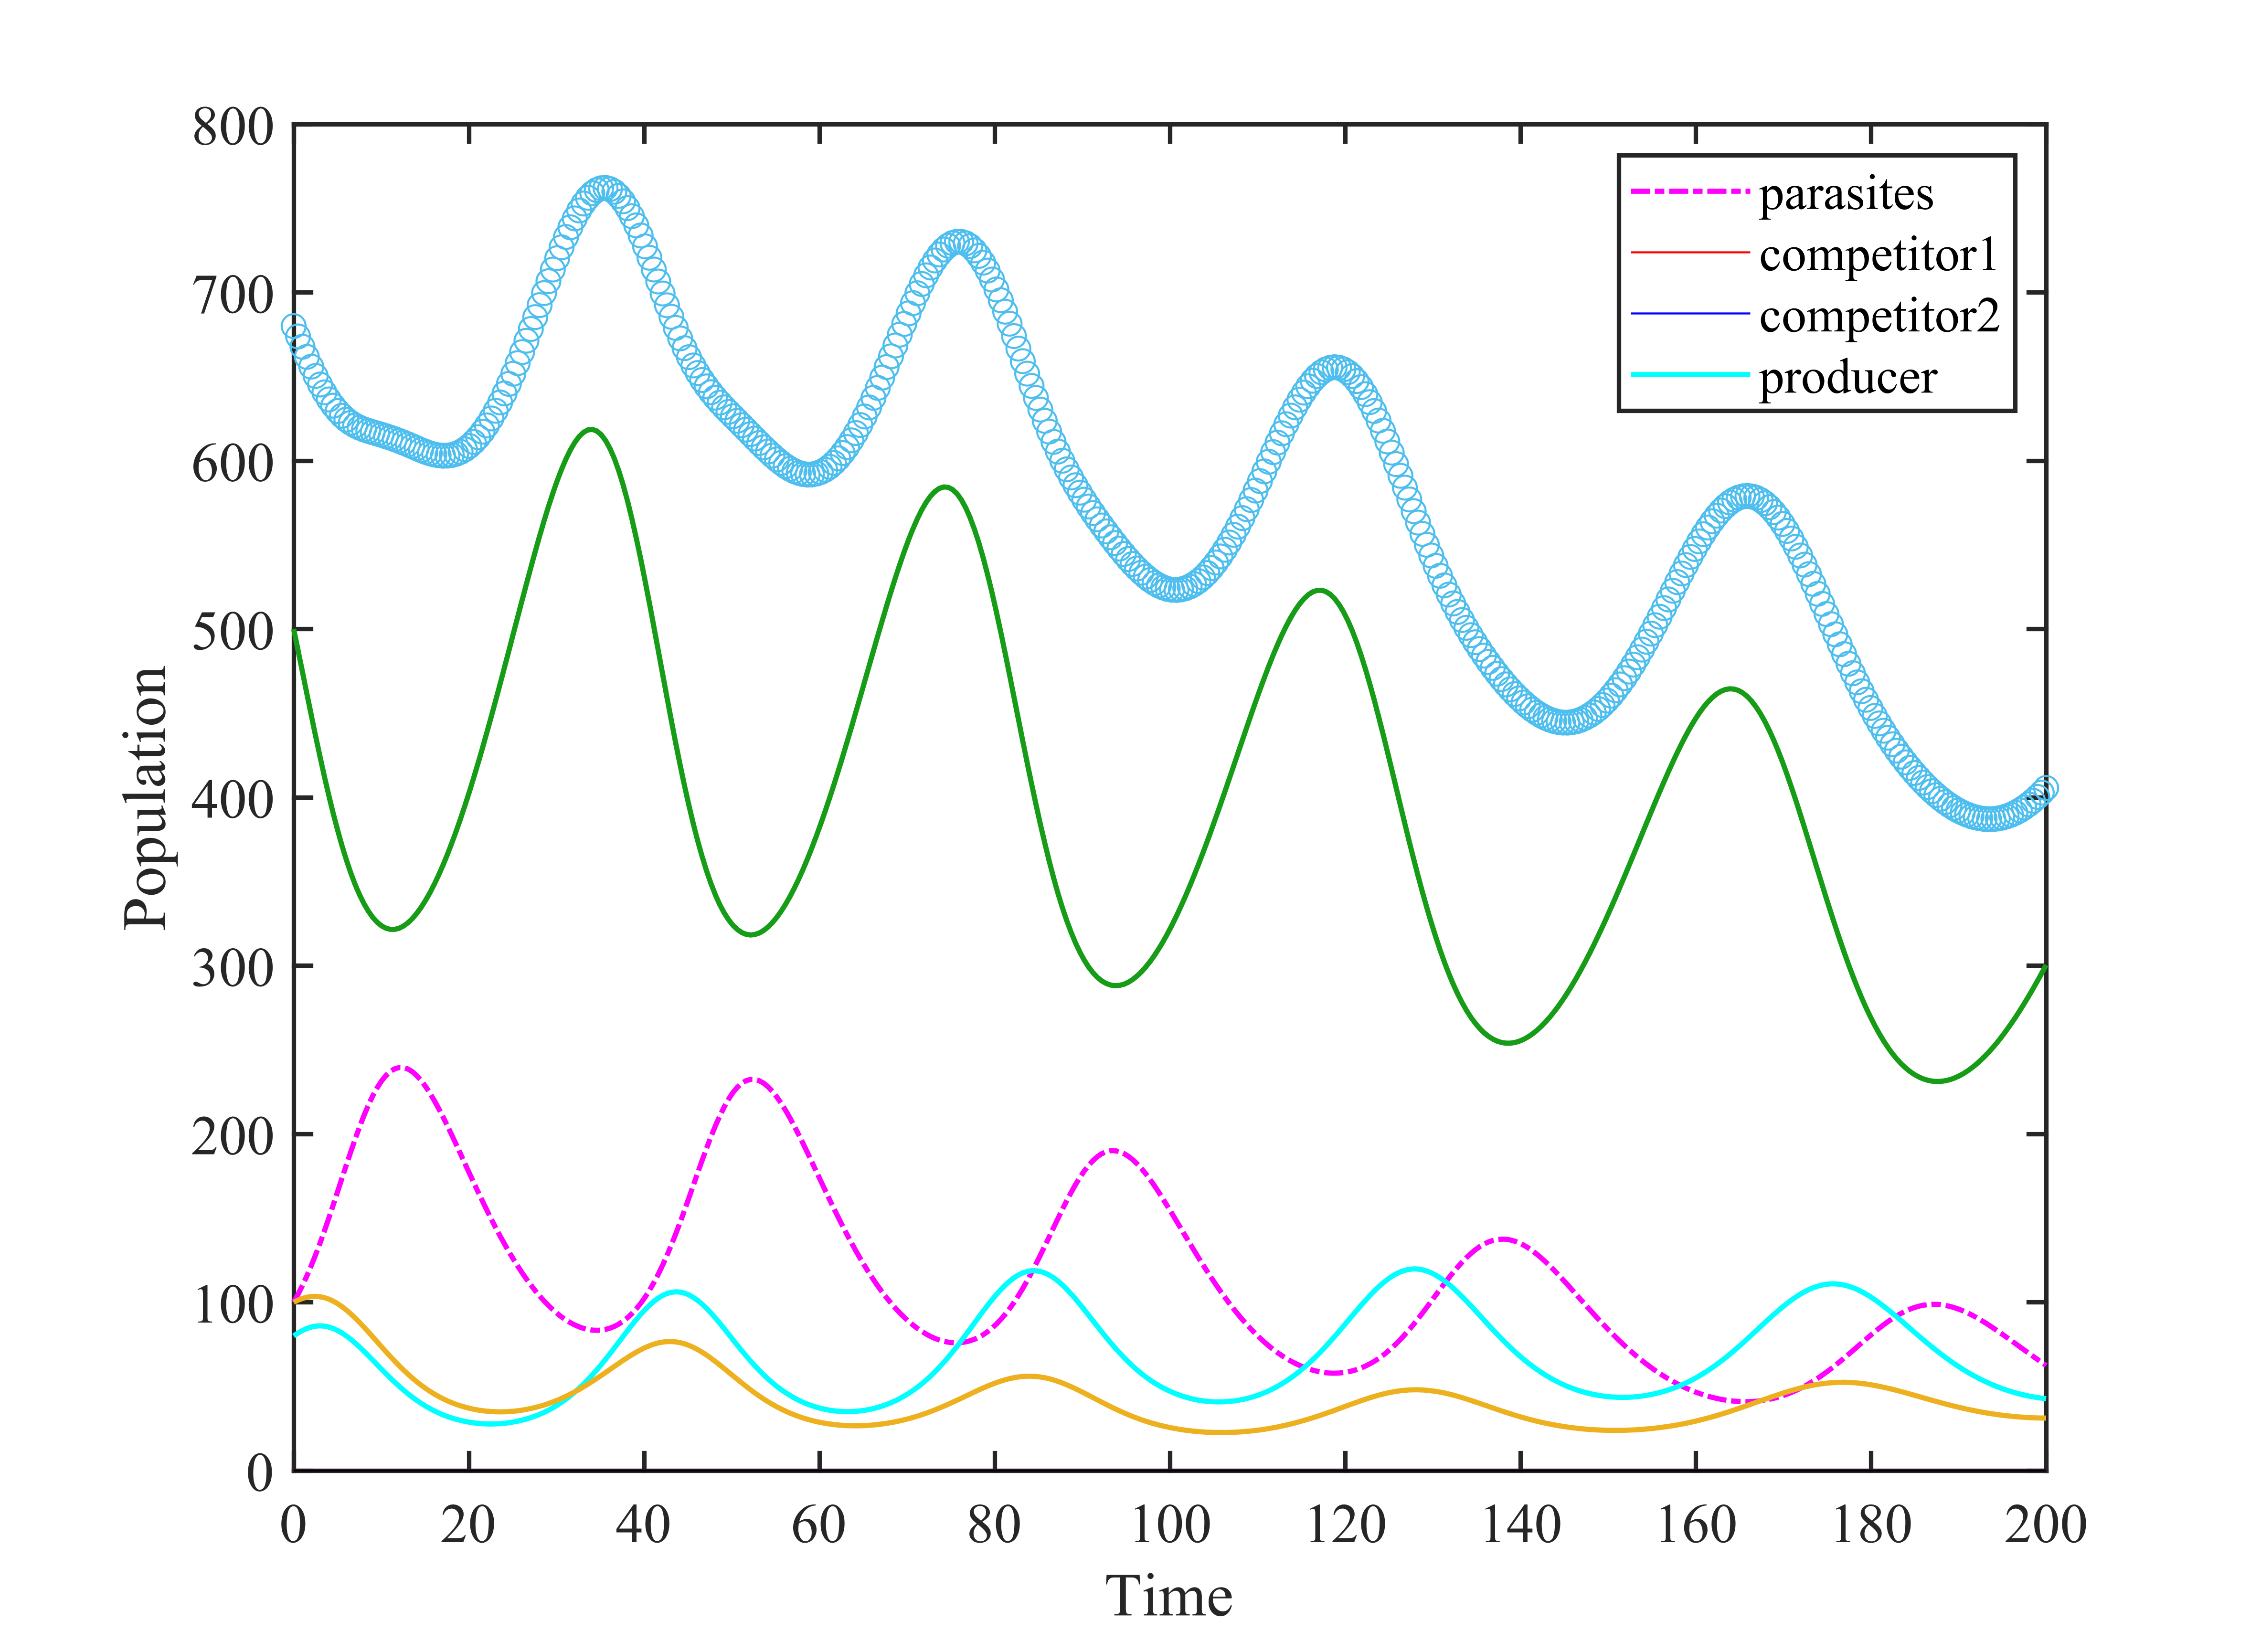
\includegraphics[width=\linewidth]{img/sum2.png}
		\caption{Sum 2 (without lamprey)}
	\end{minipage}
\end{figure}

\par

%从上面两图的对比中,可以看到具有lamprey的生态系统总生物量更稳定,而具有竞争者2的生态系统总生物量呈现下降趋势。这主要和寄生物的数量变化有关系。
It is evident from the above comparison of the two graphs that the ecosystem's total biomass with lamprey is more stable than the ecosystem's total biomass with competitor 2, which is trending downward. The shift in the quantity of parasitic organisms is mostly responsible for this.
\par
%生态系统的总生物量随时间呈现周期性波动
The total biomass of the ecosystem showed cyclical fluctuations over time, where $T_{max}$ is the total time required to run the program.\par
%其中 $T_max$是运行程序所需要的总时间
\begin{equation}
	\begin{aligned}
		\overline {TB} & =  \frac {1}{T_ {\max }} \int _ {0}^ {T_ {\max }} \sum _ {i=1}^ {n}  x_ {i}  (t)dt
	\end{aligned}
\end{equation}
%稳定性可以指抗干扰能力、恢复能力(干扰后的恢复速度)和恒定性(时间稳定性的程度)。
Stability can refer to resistance to disturbance, resilience (the rate of recovery after disturbance), and constancy (degree of temporal stability)\upcite{4}

%我们知道生态系统总生物量随时间的变化和生态系统稳定性有关,变化越小,生态系统越稳定。一般来说,我们可以使用总生物量的标准差来衡量其变化,但标准差受到数据均值和测量维度的影响。为了消除这种影响,我们定义了一个无量纲指标:总生物量的变异系数(CoV):
\par
We know that the stability of an ecosystem is correlated with its total biomass change over time; the smaller the change,the more stable the ecosystem. Generally speaking, the standard deviation of total biomass may be used to gauge change; however, the measurement's size and the data mean have an impact on the standard deviation. We define a dimensionless measure, the coefficient of variation (CoV) of total biomass, to remove this effect:\par

\begin{equation}
	\begin{aligned}
		 CoV &=  \frac {std(TB)}{TB} & =  \frac{\sqrt{\int_{0}^{T_{\max}} (TB(t) - \overline{TB})^2 \, dt}}{\overline{TB}} 
	\end{aligned}
\end{equation}
%在物理学中,我们用‘熵’来衡量系统的无序程度,Shannon-Wiener指数[引用] 是一个受熵概念启发的物种均匀度度量:在一个群落中,每个物种的平均数量是 $\overline{X_i} = \int _ {0}^ {T_ {\max }}\frac{x_i(t)}{T_{max}}dt$ 总生物量如上所述为$\overline{TB}$。 定义Shannon-Wiener index为:
\par
In physics, we use 'entropy' to measure the degree of disorder in a system, and the Shannon-Wiener index\upcite{5} is a measure of species evenness inspired by the concept of entropy: in a community, the average number of each species is $\overline{X_i} = \int _ {0}^ {T_ {\ max }}\frac{x_i(t)}{T_{max}}dt$ The total biomass is $\overline{TB}$ as previously mentioned. Define the Shannon-Wiener index as:
\par
\begin{equation}
	\begin{aligned}
		H &= \sum_{i=1}^{n}-\frac{\overline{x_i}}{\overline{TB}}log\frac{\overline{x_i}}{\overline{TB}}
	\end{aligned}
\end{equation}
\par
%由其表达式可知,index在各物种占比相同时达到最大值。分布越不均匀,Shannon-Wiener index越小。因此为了衡量相对均匀度定义Pielou指数:
According to its formulation, when the percentage of each species is the same, the index reaches its maximum value. The Shannon-Wiener index decreases with increasing distributional unevenness. Consequently, establish the Pielou index to gauge relative homogeneity:\par
\begin{equation}
	\begin{aligned}
		J &=\frac{H}{log_n}
	\end{aligned}
\end{equation}
%This is a value between [0,1],用来衡量当前均匀度和所能达到最大均匀度之间的关系。
\par
This number, which ranges from 0 to 1, represents the connection between the current uniformity and the highest possible uniformity.
 \begin{figure}[htbp]  %h此处,t页顶,b页底,p独立一页,浮动体出现的位置
	\centering  %图表居中
	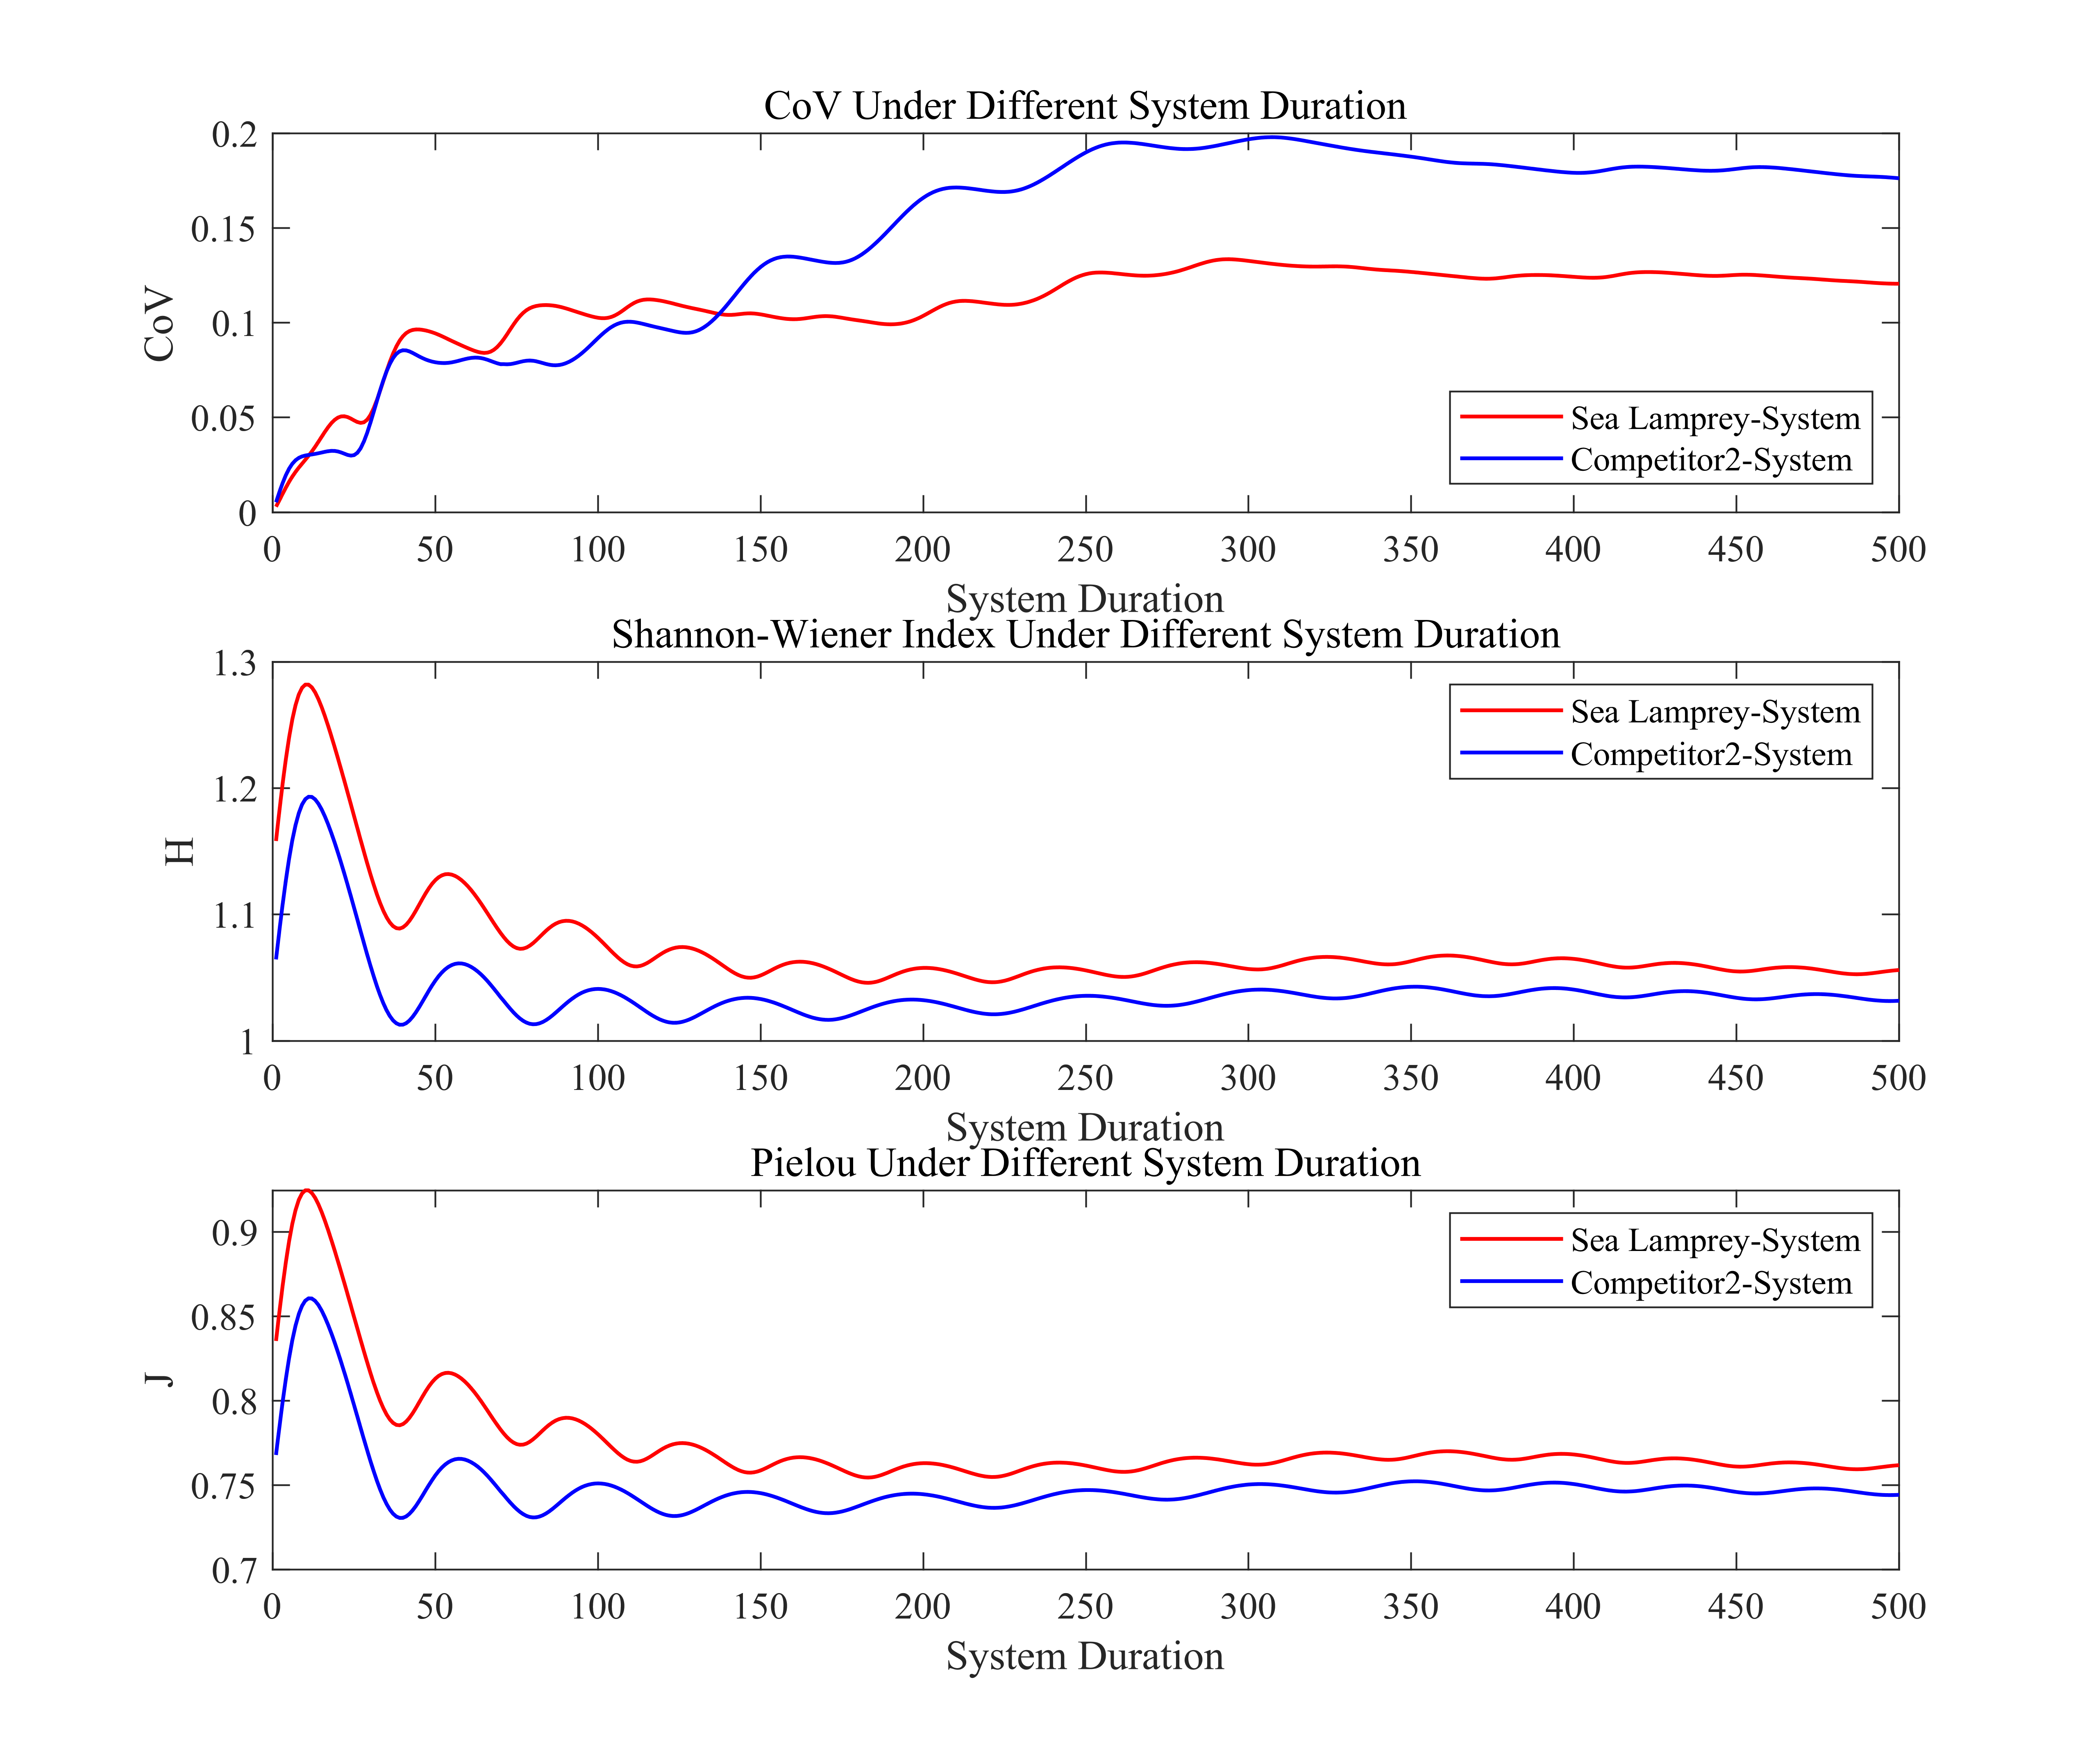
\includegraphics[width=.9\textwidth]{img/lam.png} %图片的名称或者路径之中有空格会出问题 
	\caption{Stability indicators} % 图片标题 
\end{figure}
\vspace{-0.8cm}
\par
%结果表明,生态环境的稳定性受益于适应性性别比例变化的lamprey,虽然物种在生态系统的部分并不均匀,但总生物量的变化幅度会减小,与定性分析所得结果一致,体现了模型的合理性。
The results(figure 17) demonstrate that adaptation sex ratio changes contribute to the stability of the ecosystem and that, despite species heterogeneity in the ecosystem, the magnitude of changes in total biomass decreases. These findings are in line with the findings of the qualitative analyses and support the viability of the model.\par
\subsection{Explore the advantages offered to other species.}
%在前面模型的基础上,我们已经得出结论,lamprey这种适应性性别比例变化有助于提高对生态环境的适应增加生存机会。不同物种之间的相互作用各不相同,有的物种竞争更为激烈,而有的物种之间以互利共生为主。为了探究lamprey对其他物种如寄生虫提供的优势,需要了解lamprey和寄生虫之间的关系。
Based on the prior model, we concluded that the adaptive sex ratio shift in lampreys enhances their ability to adjust to their environment and increases their chances of surviving. Different species interact differently; some are more competitive than others, while some are dominated by symbiotic relationships that are mutually beneficial. Exploring the interaction between lamprey and parasites is necessary to investigate the benefits lamprey offers to other species, such as parasites.\par
%根据Megan A. Shavalier等人的研究,至少有46种寄生虫已被记录在lamprey中。我们将寄生虫对lamprey的寄生行为看作另一种特别的捕食行为,并运用在上一问中建立的模型。
According to Megan A. Shavalier et al\upcite{6}, at least 46 species of parasites have been documented to be found on lamprey.We consider the parasitic behavior of parasites on lamprey as another special type of predatory behavior and apply the model developed in the previous question. \par
%同样的我们建立对比模型,在多物种模型中分别去除lamprey和竞争者1,以探究它们对寄生虫生物量的影响。
To investigate their impacts on parasite biomass, we similarly constructed comparison models in which competitor 1 and lamprey were removed individually from a multispecies model. \par

\begin{figure}[htbp]
	
	\begin{minipage}[b]{0.5\linewidth}
		\centering
		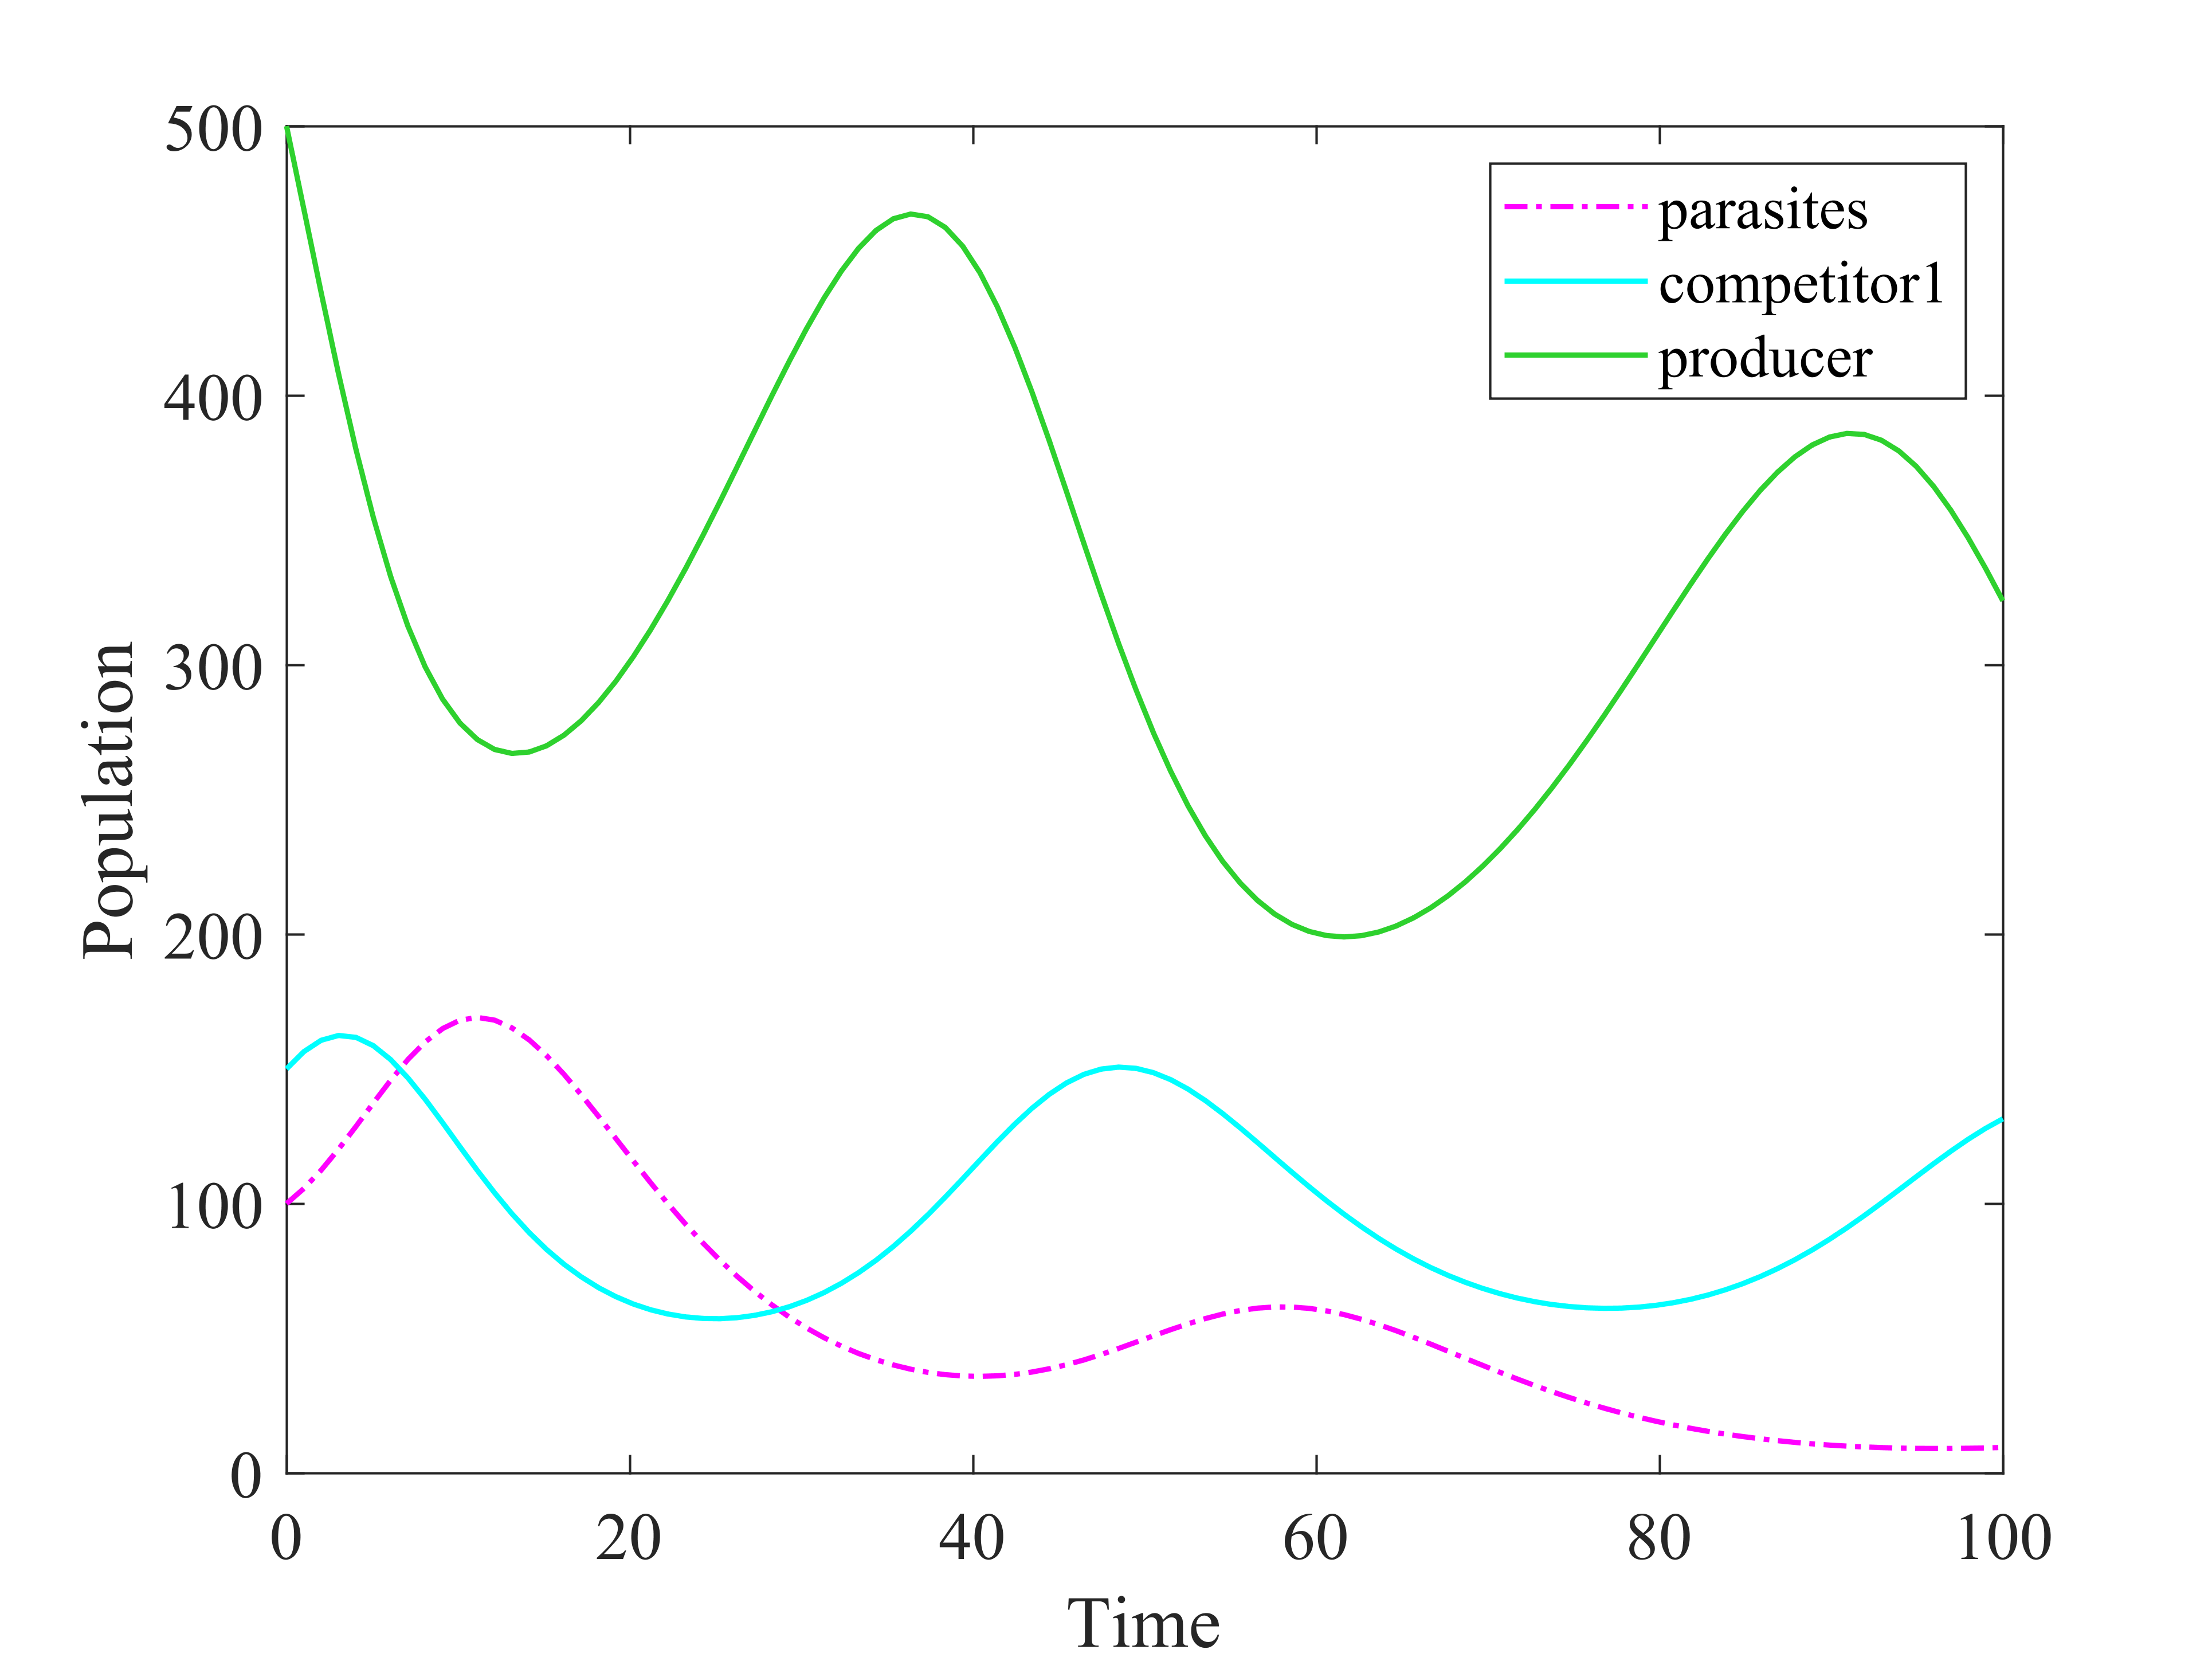
\includegraphics[width=\linewidth]{img/nolamprey.png}
		\caption{parasites,com1,product}
	\end{minipage}
	\begin{minipage}[b]{0.5\linewidth}
		\centering
		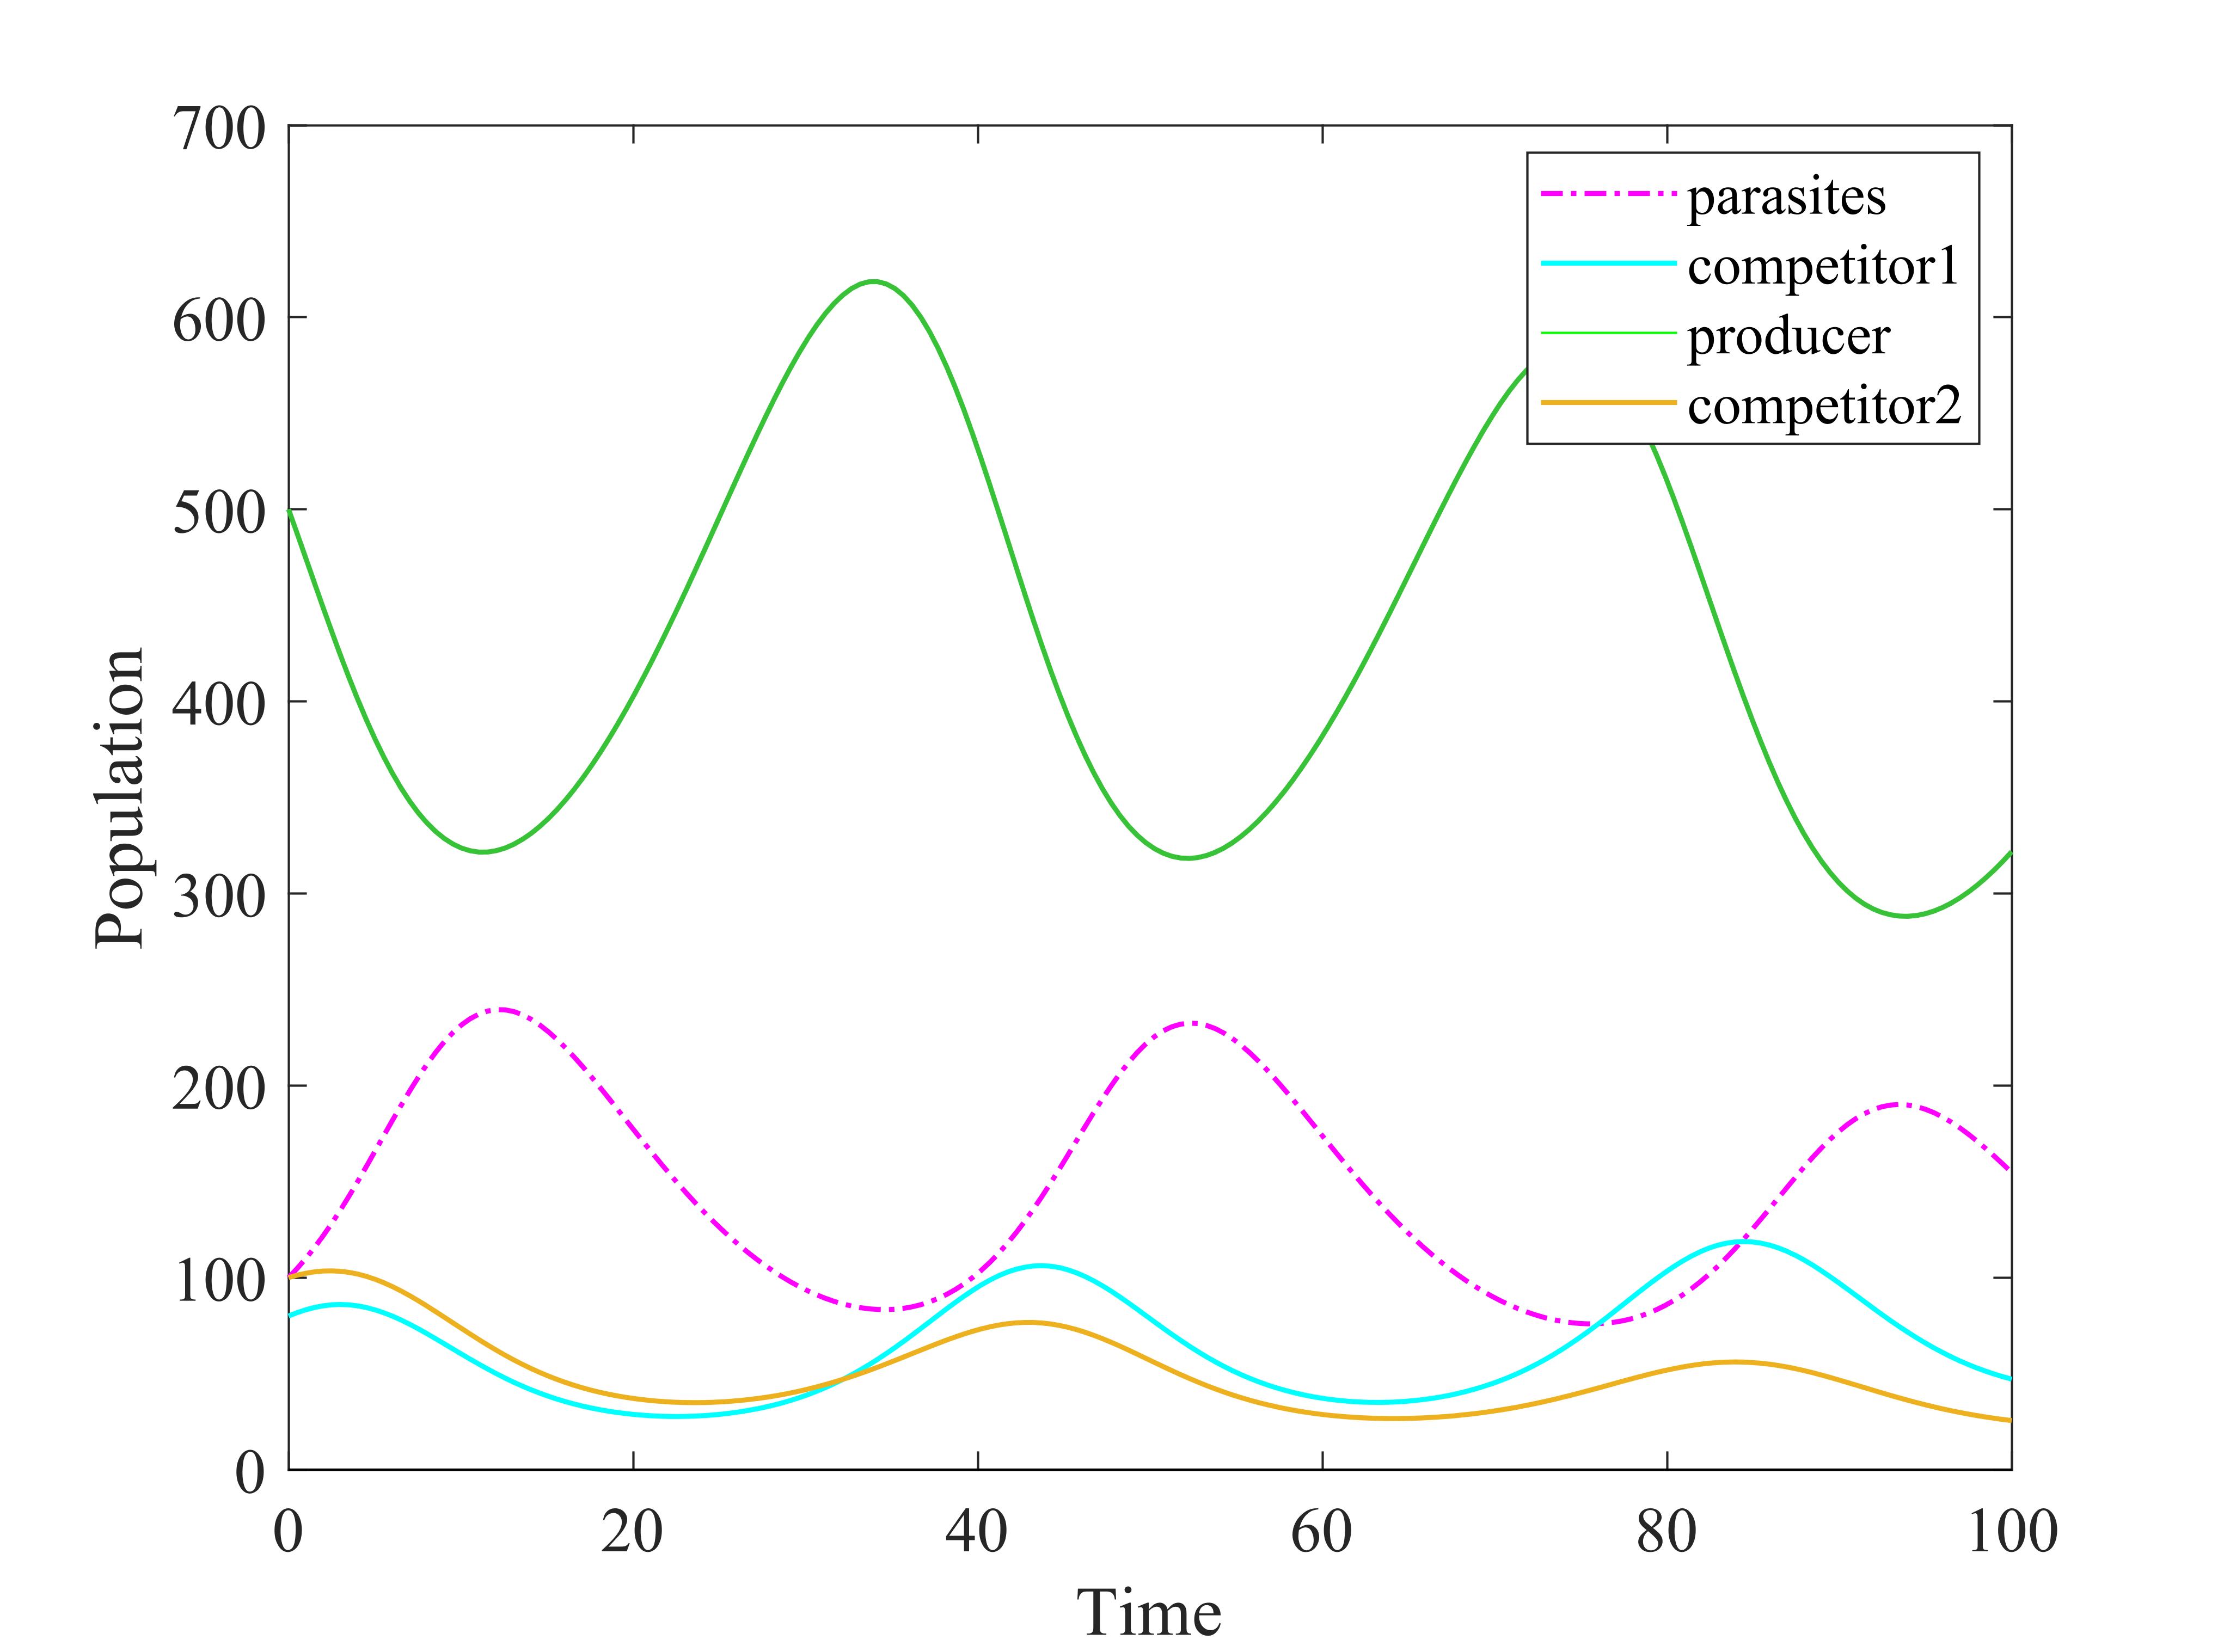
\includegraphics[width=\linewidth]{img/nolamprey2-17071503179402.png}
		\caption{parasites,com1,product,com2}
	\end{minipage}
\end{figure}
\begin{figure}[htbp]  %h此处,t页顶,b页底,p独立一页,浮动体出现的位置
	\centering  %图表居中
	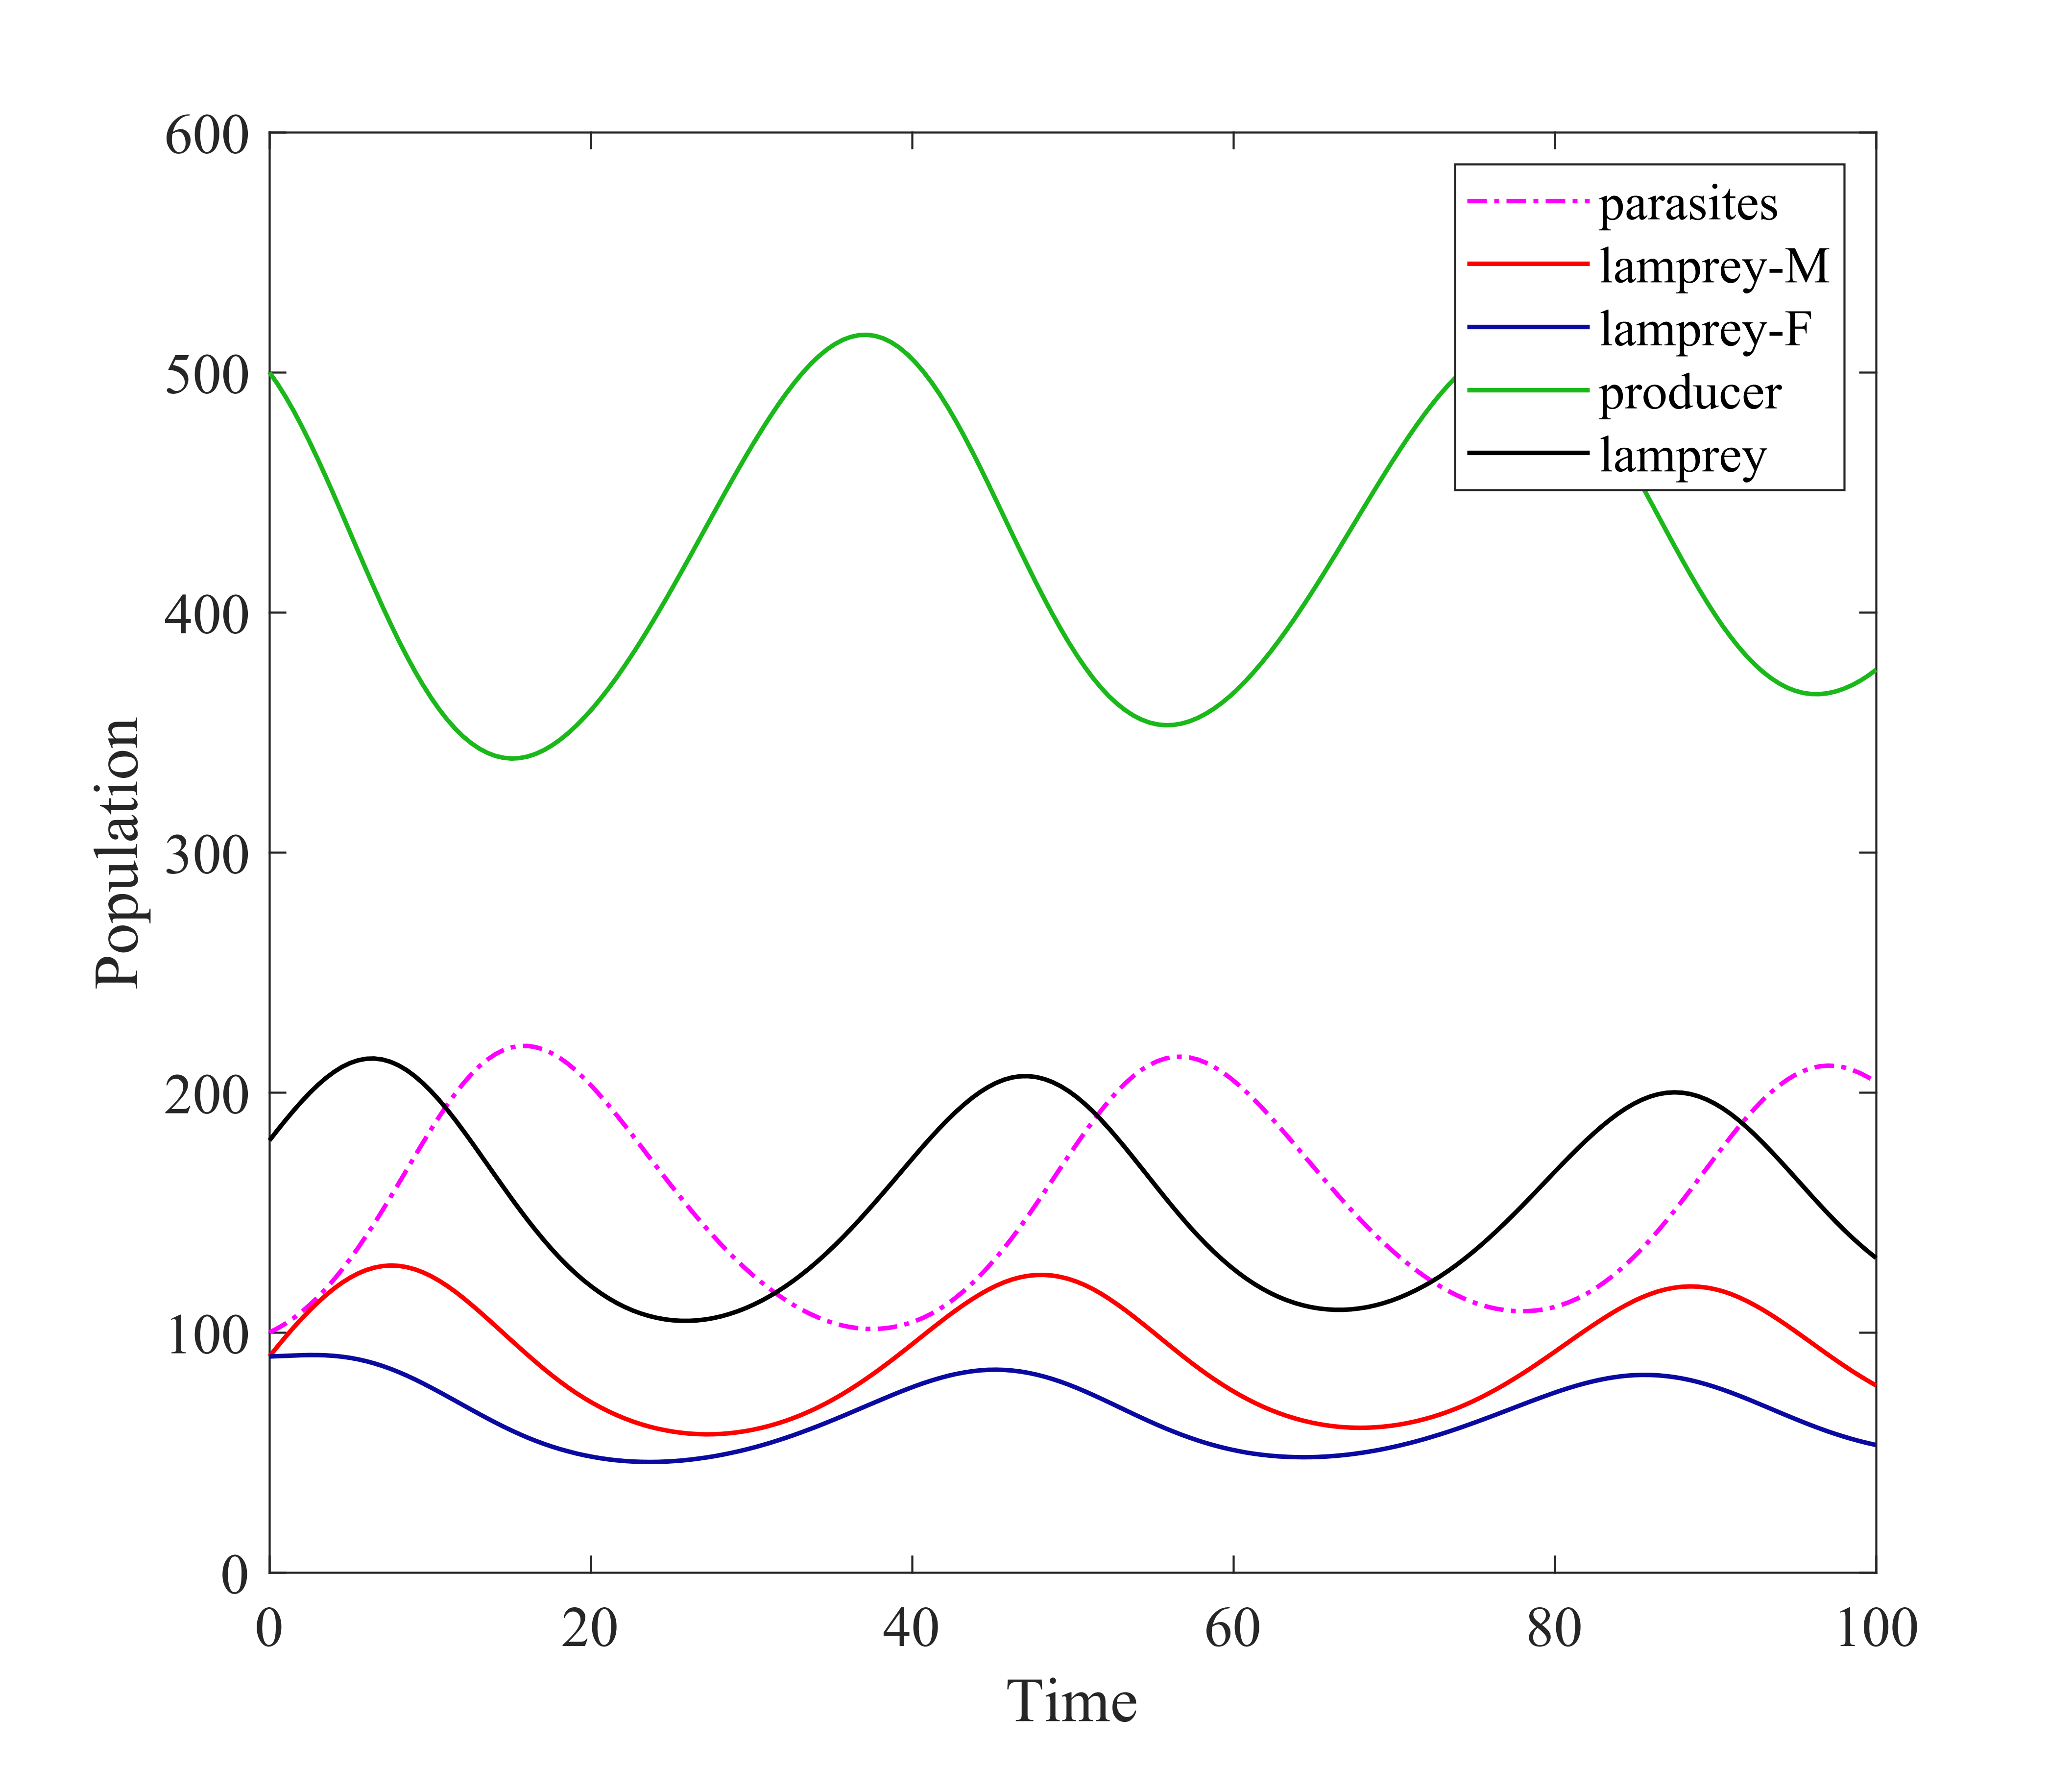
\includegraphics[width=.9\textwidth]{img/nocomp.png} %图片的名称或者路径之中有空格会出问题 
	\caption{parasites,lamprey, male, female, product} % 图片标题 
\end{figure}

\par

%从图中我们可以得到以下结论:
From the figure 18, figure 19, figure 20, we can draw the following conclusions:\par
%在相同情况下竞争者1更难以维持寄生虫的生存,而lamprey可以给寄生虫提供相对更优越的生存环境。这可能是由于lamprey在种群扩张的过程中,性别比例逐渐失衡,繁殖潜力降低,抑制了种群扩张的速度和最大值,同理在种群缩小的过程中,繁殖潜力随性别比例的变化而提高,抑制了种群缩小的速度和最大值,因此lamprey拥有更短的迭代周期和更稳定的种群数量,这为寄生虫提供了稳定的食物来源。

%lamprey生物量提高对食物资源的需求更低,有适应性性别比例的lamprey的生态环境中,生产者的数量更多。

\begin{enumerate}[\bfseries (1).]
	\item Under identical conditions, competitor 1 finds it more difficult to sustain the parasite's existence, whereas lamprey can offer a somewhat more conducive environment.One possible explanation for this might be the increasing imbalance in the sex ratio of lampreys that occurs as the population grows, which lowers their capacity for reproduction and limits the rate and maximum value of population growth,similarly, as the population shrinks, reproductive capacity rises with the sex ratio, limiting thsimilarlye rate and absolute value of population decline. As a result lamprey has shorter iteration cycles and more stable population sizes, which provide a stable food source for the parasite.\par
	
	\item The increased biomass of lamprey has a lower demand for food resources, and ecosystems with adapted sex ratios of lamprey have a greater number of producers.
\end{enumerate}
\par

%寄生虫种群的稳定抑制了海七鳃鳗与竞争者1的种群规模,进一步为生产者提供了更优良的生存空间,生产者种群更大会给整个生态系统带来更丰富的资源和更强的稳定性
The sea lamprey and competitor 1's population sizes are suppressed as parasite numbers stabilize, giving producers more room to live. Larger producer populations mean richer resources and more stability for the ecosystem as a whole.\par
\section{Sensitivity Analysis and Stability Analysis}
%对生产者自然增长率的模型灵敏度分析
\subsection{Sensitivity analysis of the model for the producers' natural growth rate}
%生产者作为一个生态系统中的原始能量供给者,对生态系统生物量、迭代情况与稳定性都有着重要作用,生产者能提供的能量大小取决于其自然增长率,通过计算不同的自然增长率下模型的稳定性来评估模型的灵敏度。
\par
Producers, as the original energy suppliers in an ecosystem, play an important role in ecosystem biomass, iteration and stability. The amount of energy a producer can provide depends on its natural growth rate, and the sensitivity of the model is assessed by calculating the stability of the model at different natural growth rates.
\par
\begin{figure}[htbp]  %h此处,t页顶,b页底,p独立一页,浮动体出现的位置
	\centering  %图表居中
	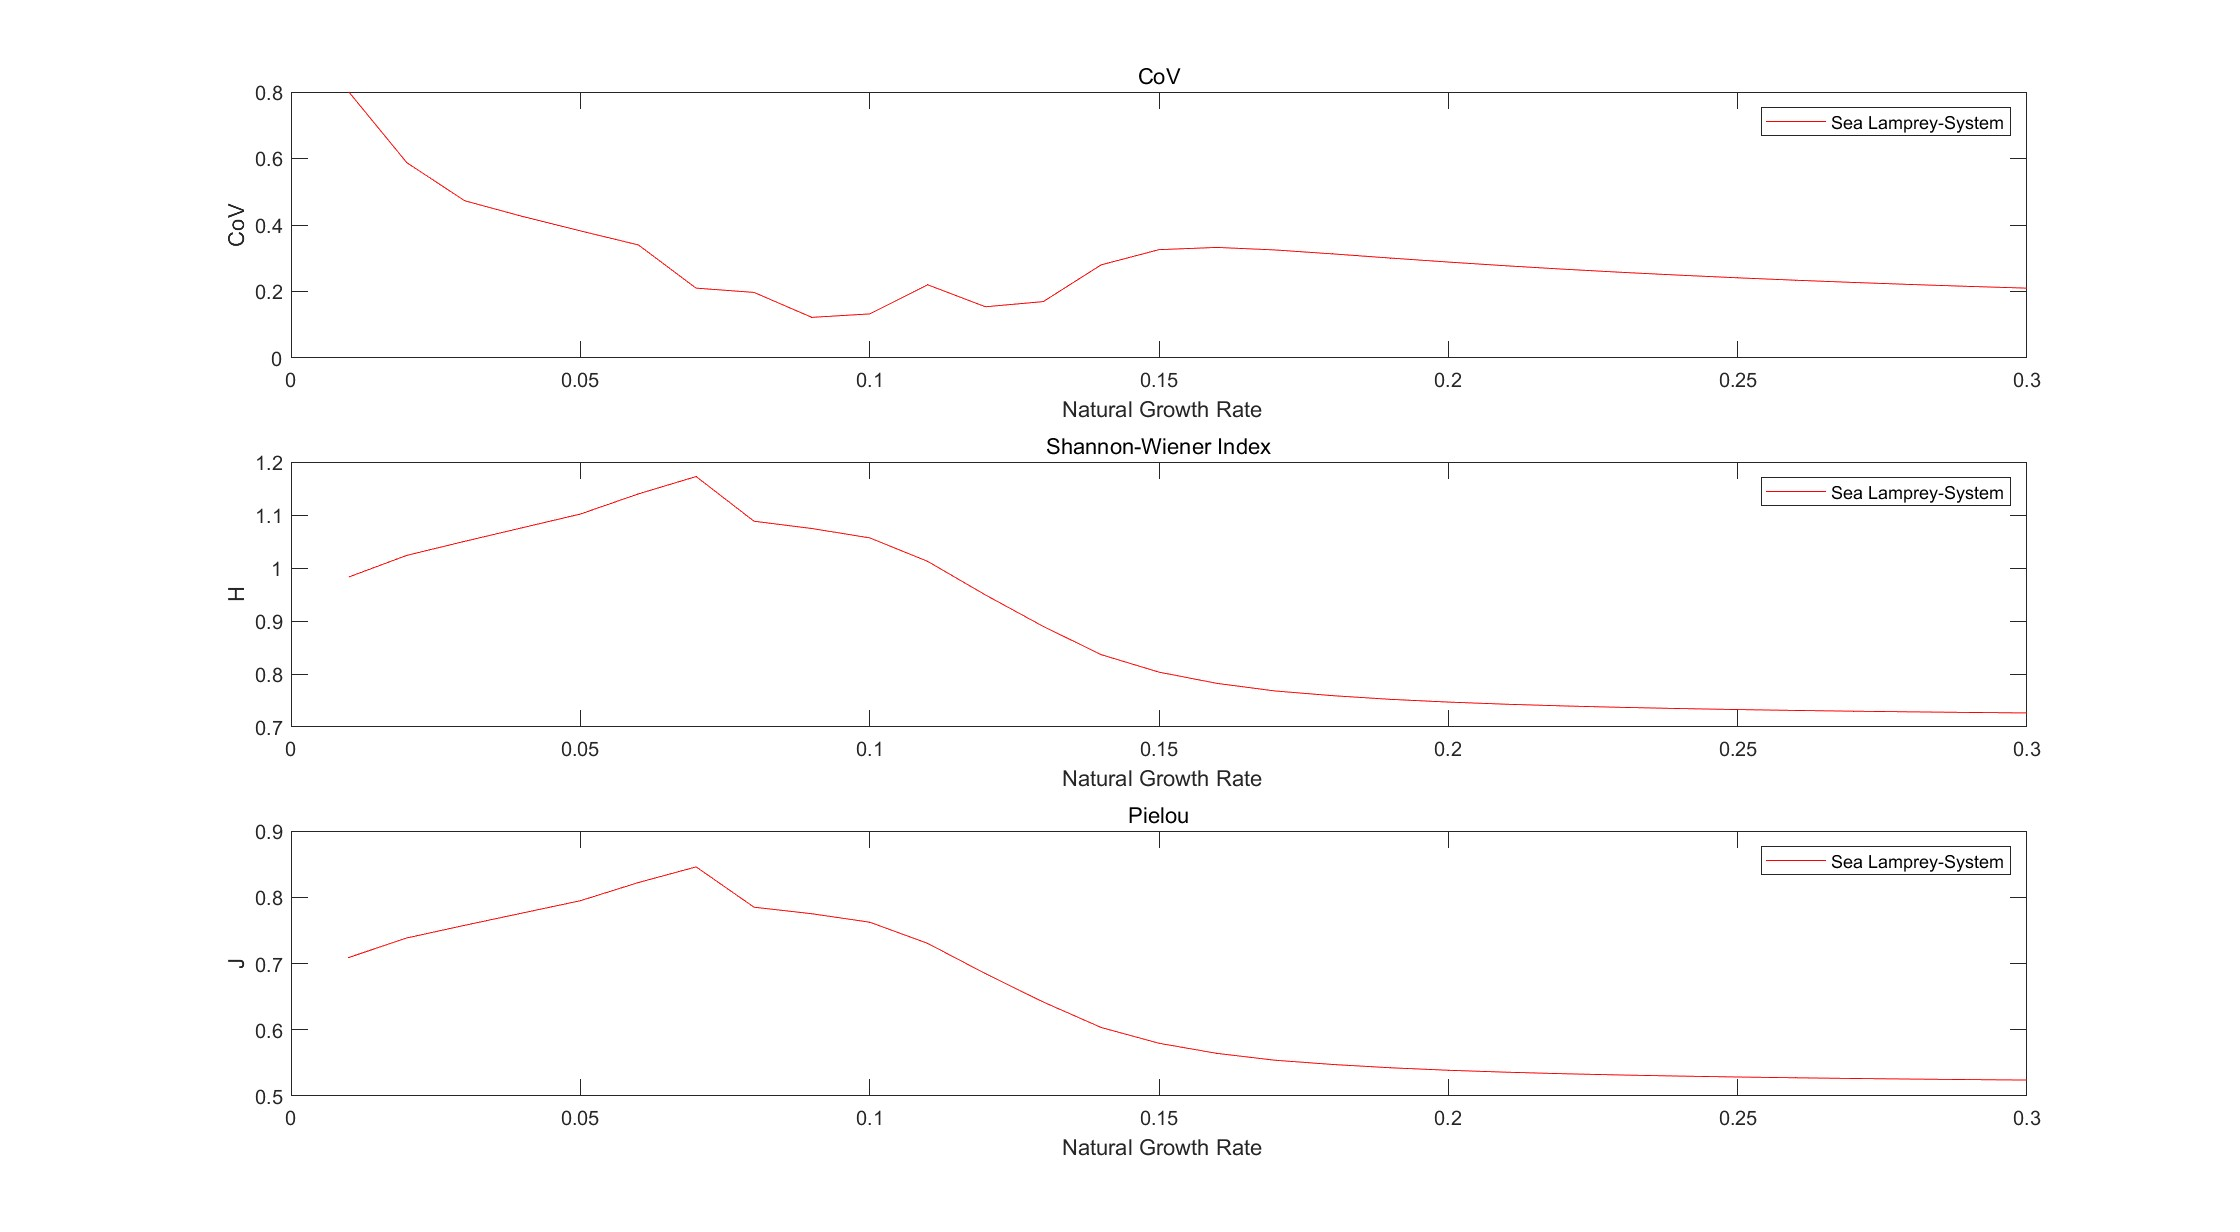
\includegraphics[width=.9\textwidth]{img/ngr.jpg} %图片的名称或者路径之中有空格会出问题 
	\caption{Sensitivity analysis  for the producers' natural growth rate} % 图片标题 
\end{figure}
\par
%在自然增长率处于 [0.01, 0.15] 的区间上模型较为稳定,超过0.15后过高的自然增长率会导致系统崩溃。
From the figure 21, it is obviously that the model is more stable in the interval [0.01, 0.15] where the natural rate of growth is higher than 0.15, causing the system to break down.\par
%对七鳃鳗种群初始数量的模型灵敏度分析
\subsection{Model sensitivity analysis of the initial population size of the lamprey}
%七鳃鳗种群的初始数量对整个生态系统的迭代状况也有很重要的作用,通过计算短时间内不同的自然增长率下模型的稳定性来评估模型的灵敏度。
\par
The initial size of lamprey's population also plays an important role in the iterative status of the whole ecosystem, and the sensitivity of the model was assessed by calculating the stability of the model at different natural growth rates over a short period of time.\par
\begin{figure}[htbp]  %h此处,t页顶,b页底,p独立一页,浮动体出现的位置
	\centering  %图表居中
	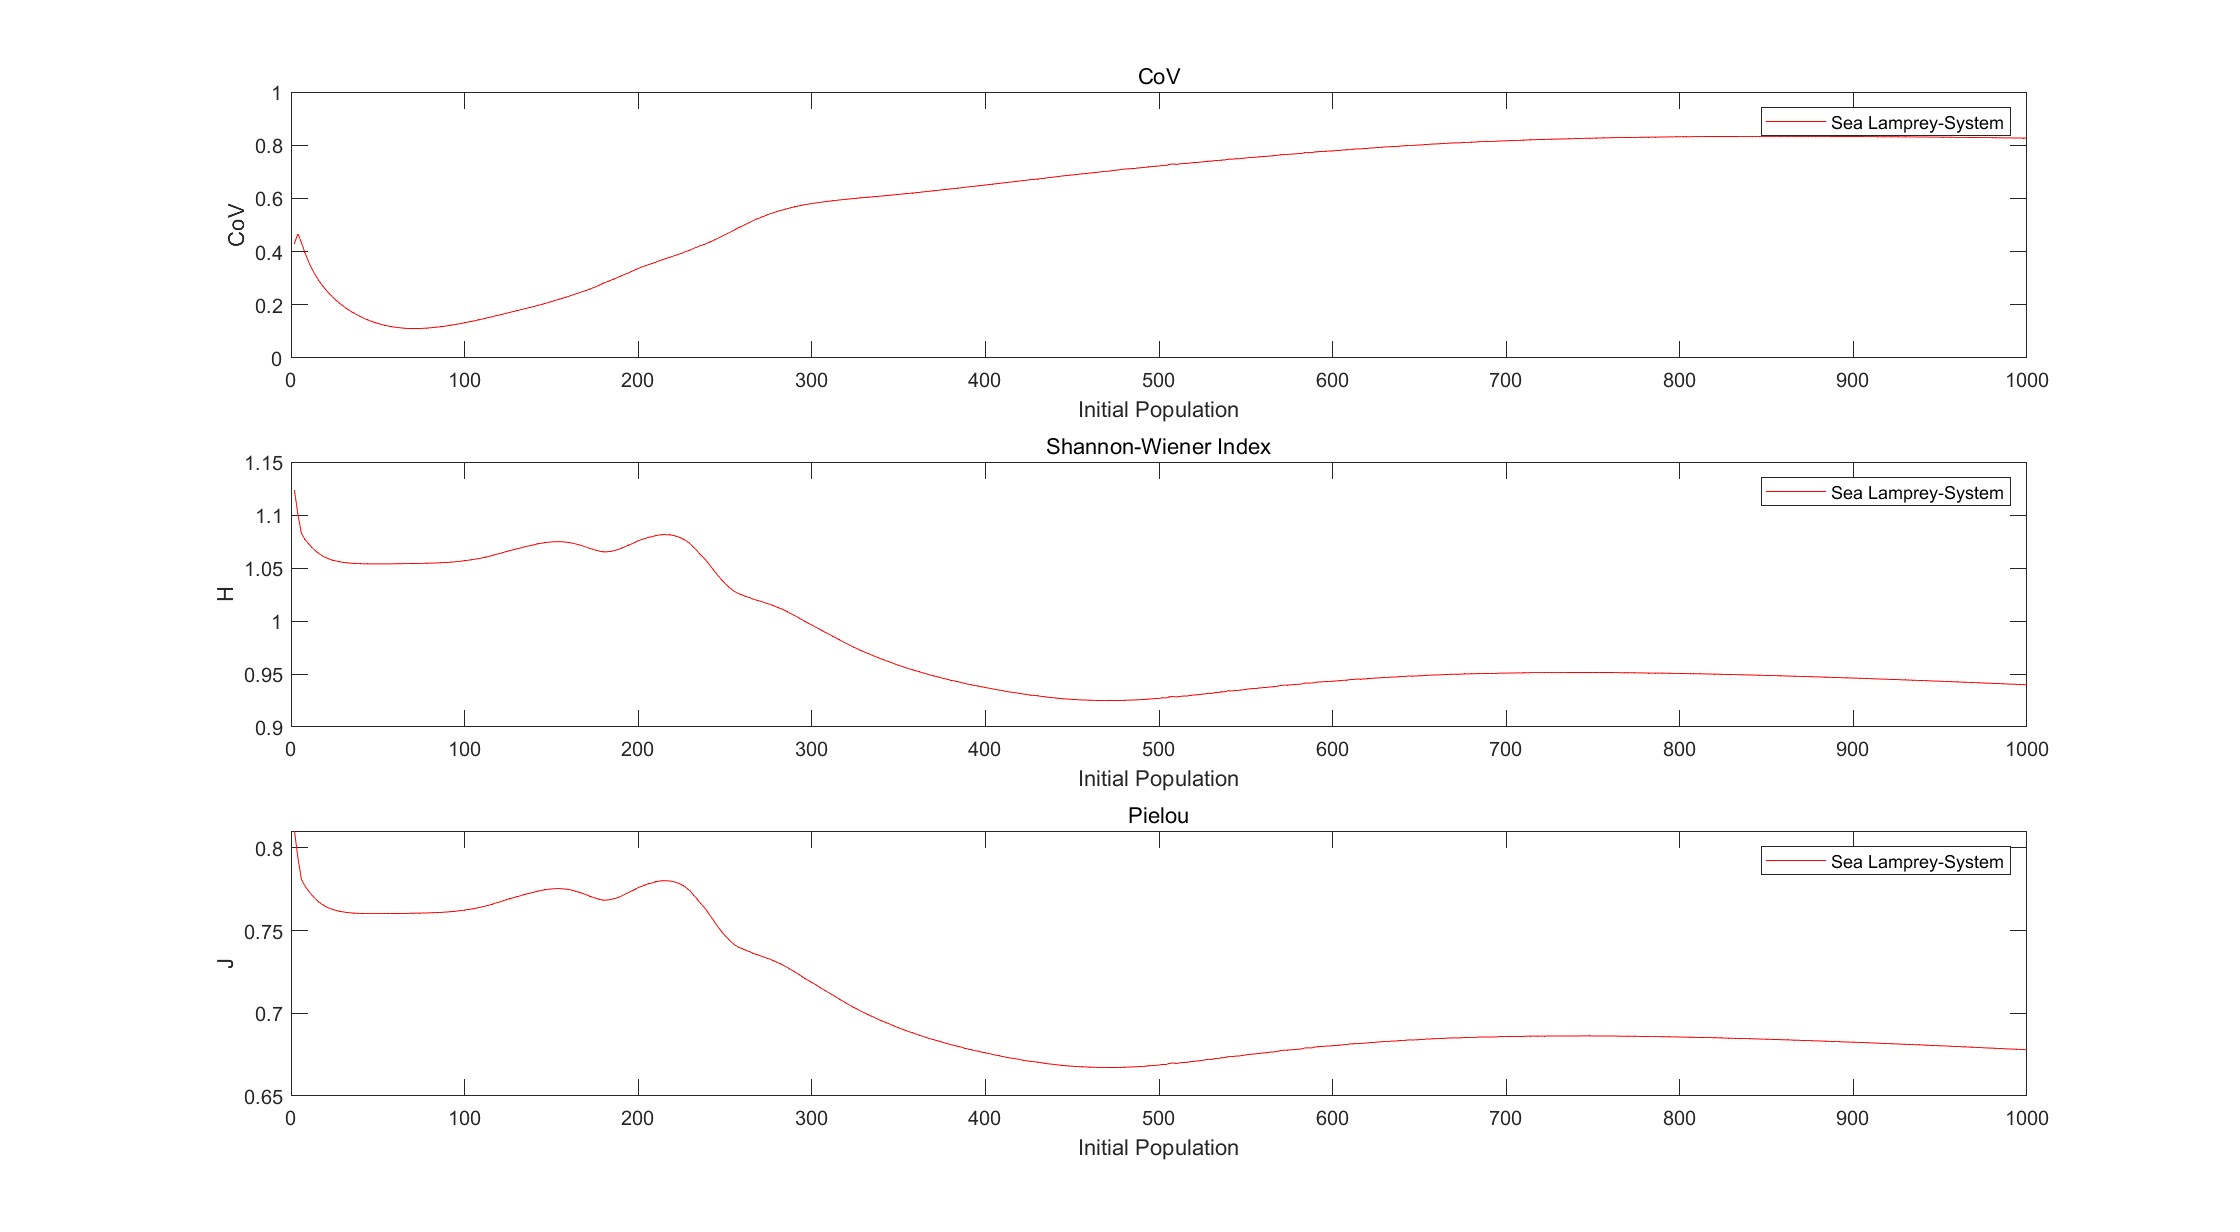
\includegraphics[width=.9\textwidth]{img/ipr-1707158411741-12.jpg} %图片的名称或者路径之中有空格会出问题 
	\caption{Model sensitivity analysis of the initial population size of the lamprey} % 图片标题 

\end{figure}
\par
%在短时间内,种群初始数量处于 [20, 300] 范围内模型较稳定,过高的初始数量会导致七鳃鳗竞争物种与生产者因生存压力过大而快速灭绝,故而系统稳定性下降并收敛。受限于效率问题,此处只考察了较短时间内生态系统稳定性的灵敏度,由于初始种群数量的变化也可能改变系统的迭代周期与趋势,增长系统的迭代时长可能导致结果有所不同。
From the figure 22, In a short period of time, the initial population size is in the range of [20, 300] the model is more stable, too high initial number will lead to lamprey competing species and producers due to the survival pressure is too lamprey large and rapid extinction, so the stability of the system decreases and convergence.Due to efficiency issues, only the sensitivity of ecosystem stability over a shorter period of time is examined here, and since changes in initial population size may also change the iteration period and trend of the system, the iteration length of growing the system may lead to different results.
\par
%对七鳃鳗种群环境承载力的模型灵敏度分析
\subsection{Model sensitivity analysis of the environmental carrying capacity of lamprey populations}
%环境承载力决定了七鳃鳗种群能够扩张的上限,通过计算不同环境承载力下模型的稳定性来评估模型的灵敏度。
Environmental carrying capacity determines the upper limit of how much the lamprey population can expand, and the sensitivity of the model was assessed by calculating the stability of the model under different environmental carrying capacities.\par
\begin{figure}[htbp]  %h此处,t页顶,b页底,p独立一页,浮动体出现的位置
	\centering  %图表居中
	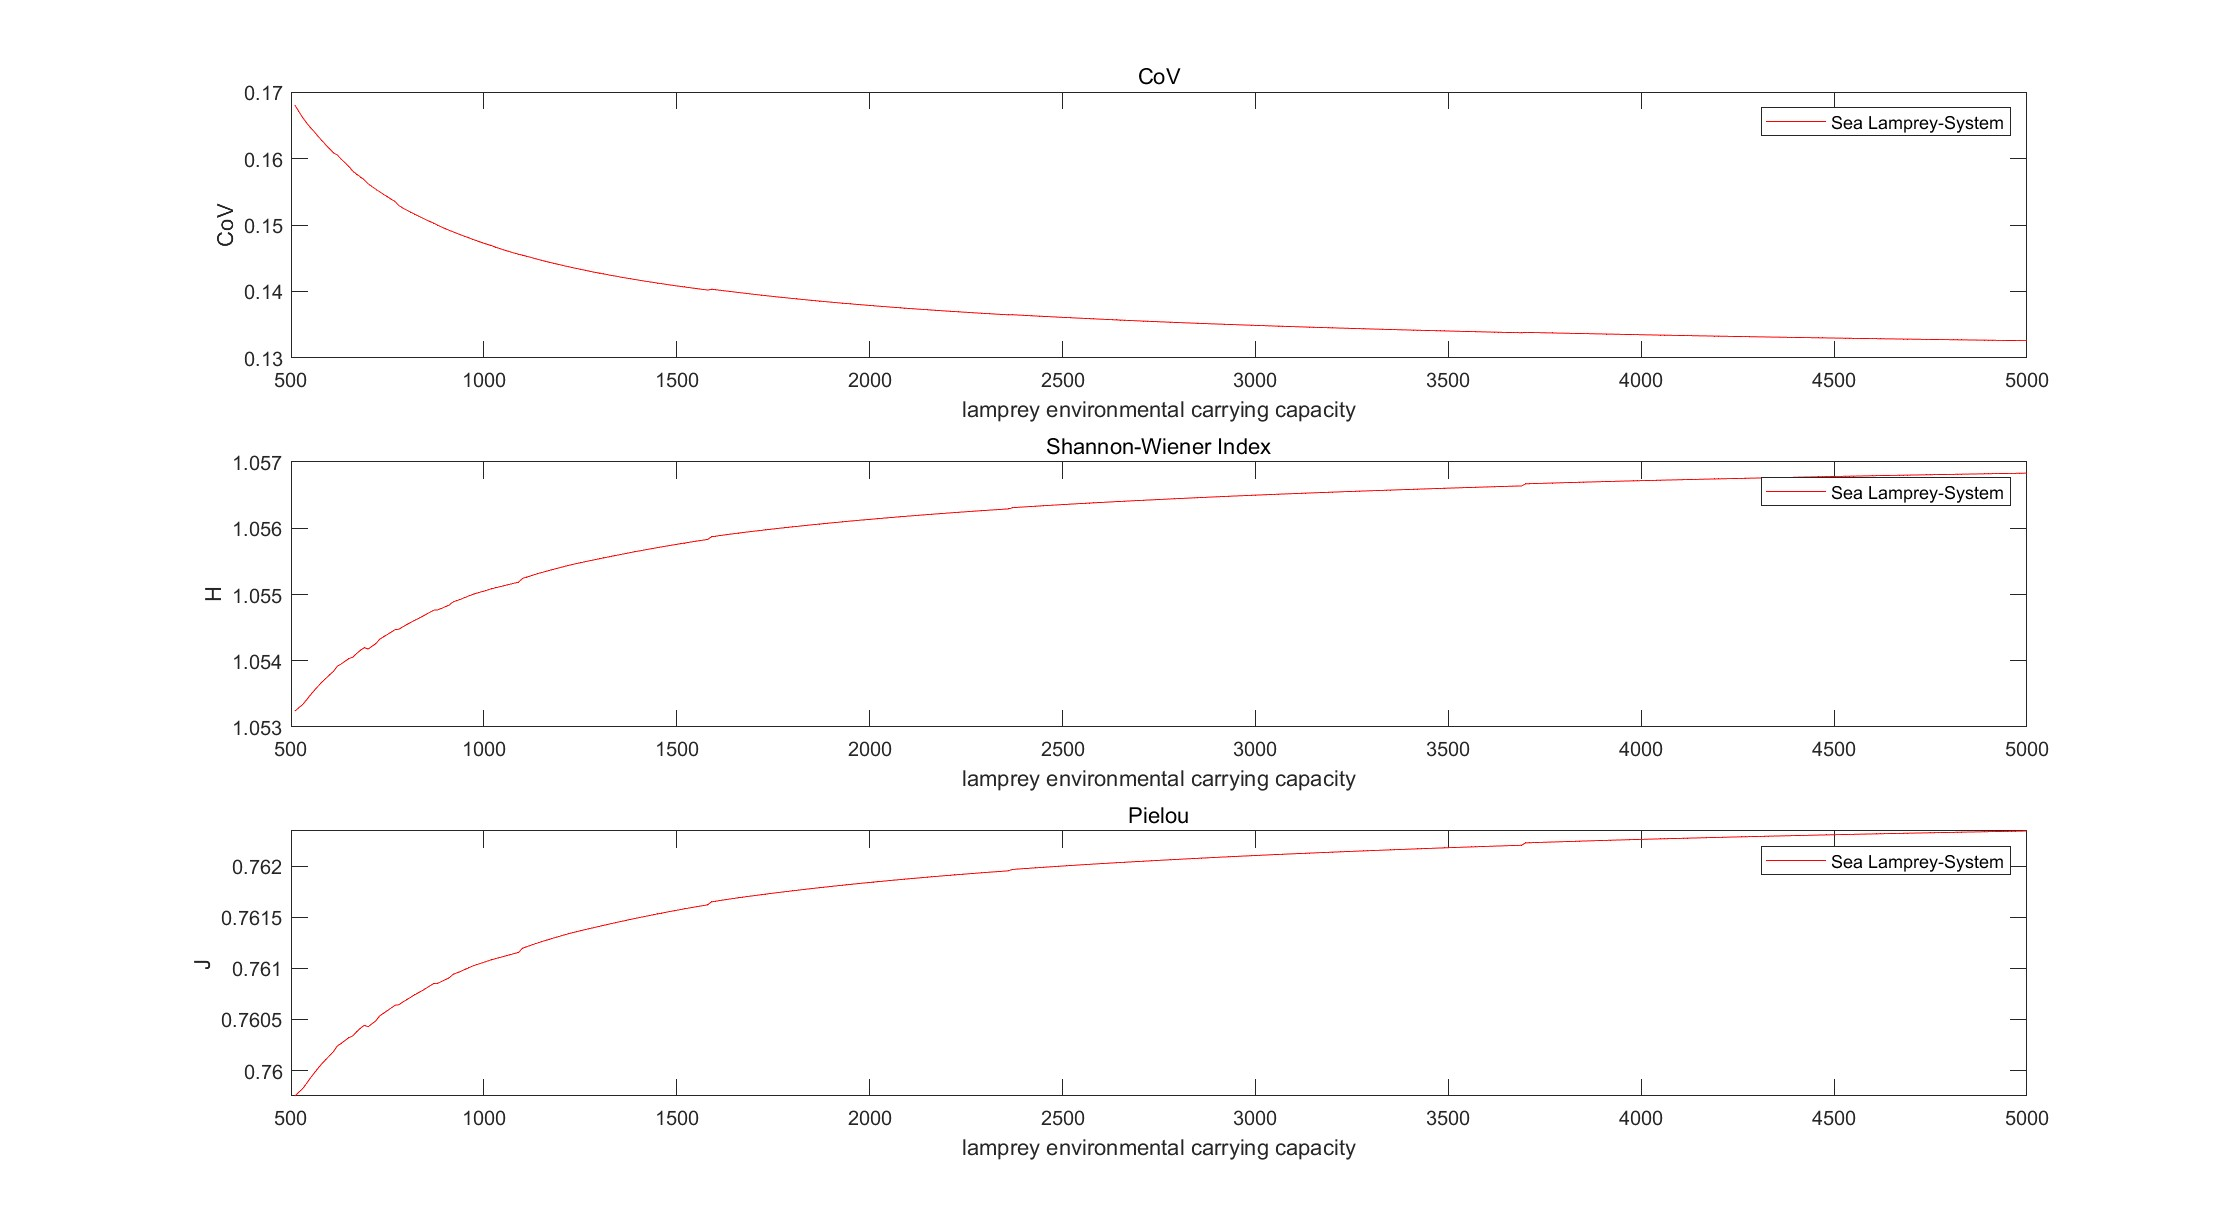
\includegraphics[width=.9\textwidth]{img/ikr.jpg} %图片的名称或者路径之中有空格会出问题 
	\caption{Model sensitivity analysis of the environmental carrying capacity of lamprey populations} % 图片标题 
\end{figure}
%当环境承载力高于3000时,模型表现较为稳定,过低的环境承载力会严重限制七鳃鳗的生存,导致其快速灭绝,从生态系统中被淘汰
\par
From the figure 23, When the environmental carrying capacity is higher than 3000, the model performance is more stable, too low environmental carrying capacity will severely limit the survival of lamprey, leading to its rapid extinction and elimination from the ecosystem lamprey
\section{Strengths and Weaknesses}
\subsection{Strengths}
%(1)本团队基于lotka Volterra模型,将雄性和雌性lamprey分开考虑,并引入了捕食转化率,环境承载力等因素,创造性的构建了考虑物种相互作用,性别比例对繁殖和生长影响等多种因素的修正模型
%(2)将雌雄性别分别进行建模,可以使得物种可用性导致的性别变化对种群的真实性别比例的影响存在滞后性, 更正却
%(3)利用生物量合理构建一个模型来评价性别比例变化对生态系统的影响
%(4)在模型中,我们综合运用了许多科学的生态学模型,并在这些模型的基础上进行了一些调整,简化和修改,最终建立了我们的整体综合模型。
\begin{enumerate}[\bfseries ·]
	\item Our team utilized the lotka-Volterra model as a basis, taking into account the characteristics of male and female lamprey individually. We included variables such as predation conversion rate and environmental carrying capacity and we creatively create a revised model that considers a variety of elements, including interactions between species, the impact of sex ratio on development and reproduction, etc.
	\item Modeling the male and female sexes separately, which make it possible to account for a lag in the effect of sex changes due to species availability on the true sex ratio of a population. It is more appropriate to represent the impact of sex differences in the lamprey using separate models.
	\item Using biomass to rationalize a model for evaluating the effects of sex ratio changes on ecosystems
	\item To construct our overall comprehensive model, we combined many scientific ecological models and expanded upon them with certain tweaks, simplifications, and adjustments.
\end{enumerate}
\subsection{Weaknesses}
%(1) lotka Volterra模型为基础,构建本文的模型,忽略了部分生态系统的复杂因素,例如空间分布,鱼群迁徙,人为因素
%(2) 模型的数值解可能对于初始条件和参数选择非常敏感,因此需要进行进一步的敏感性分析。
\begin{enumerate}[\bfseries ·]
	\item This work's model was constructed based on the Lotka-Volterra model, which overlooked some of the complexities of the ecosystem, such as fish migration, geographic distribution, and human influences.
	\item The numerical solution of the model may be highly sensitive to the initial conditions and parameter choices, necessitating further sensitivity analysis is required.
	
\end{enumerate}


% 参考文献,此处以 MLA 引用格式为例
\clearpage   %另起一页继续写。这时,你最好使用“\clearpage” 
\begin{thebibliography}{99}
	\bibitem{1} Hansen, Michael J. , et al. "Population ecology of the sea lamprey (Petromyzon marinus) as an invasive species in the Laurentian Great Lakes and an imperiled species in Europe." Reviews in Fish Biology and Fisheries (2016).
	\bibitem{2} Johnson Nicholas S., Swink William D. and Brenden Travis O. 2017 Field study suggests that sex determination in sea lamprey is directly influenced by larval growth rateProc. R. Soc. B.28420170262.20170262
	\bibitem{3} Michael J. Hansen, et al. "Population ecology of the sea lamprey (Petromyzon marinus) as an invasive species in the Laurentian Great Lakes and an imperiled species in Europe." Reviews in Fish Biology \& Fisheries (2016).
	\bibitem{4} Ma, Zilong , and  H. Y. H. Chen . "Effects of species diversity on fine root productivity in diverse ecosystems: a global meta‐analysis." Global Ecology \& Biogeography (2016).
	\bibitem{5} Strong, W. L . "Biased richness and evenness relationships within Shannon–Wiener index values." Ecological Indicators (2016).
	\bibitem{6} Shavalier, Megan A. , et al. "Parasites and microbial infections of lamprey (order Petromyzontiformes Berg 1940): A review of existing knowledge and recent studies." Journal of great lakes research S1(2021):47.
	\bibitem{7} Stéphanie Boulêtreau, et al. "High predation of native sea lamprey during spawning migration." Scientific Reports 10.1(2020).
\end{thebibliography}
% \includepdf[pages={1,2}]{Memo.pdf} 
\clearpage
\section*{Appendices}
\begin{center}
\textbf{Listing : Multi-species ecosystem modeling}\par
\end{center}

\linenumbers
\begin{lstlisting}[language=Matlab]{code/question_4_2(3).m}
	
% Consider a more complex ecosystem, with four species:
% Parasites-Competitors 1+ Lamprey, three levels of the food chain
clear;
clc;
close all;

% In the initial population, lamprey and competitor 2 can only choose one
init_value = [100, 50, 50, 80, 500, 0, 0]; 
% Parasite;Male-Lamprey;Female-Lamprey;Competitor 1;Producer;Competitor 2

% time range
Time = linspace(0, 500, 1000);

% solving equations
[T1, Y1] = ode45(@question_4_2_B, Time, init_value);

function eq = question_4_2_B(T, Y) 
%{
	init_value = [100, 50, 50, 80, 500, 0, 0];
	Under this parameter set, although the number of each species does not 
	converge stably, it presents periodic stability, and there are alternate 
	changes in the proportion of population with large and small periodic competitors.
	1. Keeping other parameters constant,[a14a41] = [-2e-3 -2e-3] can make 
	the model converge slowly, and decreasing [a14a41] can accelerate convergence 
	and shorten the period.
	2. Based on this model, either the heptagill or competitor species are 
	deleted, and the same amount removed is added to the initial number 
	of the other. Looking at the model, it is found that the competitor 
	has difficulty maintaining the survival of the parasite, while the 
	heptagill can provide a relatively superior living environment for the parasite.
	%}

eq = zeros(7,1);
% Subfunctions and Parameter Definitions
A = (Y(5)+Y(6))./(1e-50+Y(2)+Y(3)+Y(4)); % 1e-50 Prevent denominator from zero
% R = alpha * ln(A + beta) + gamma; (5:3, 78%) (1:5, 50%) (1:20, 40%)
p_alpha = -0.1514;
p_beta = 0.4585;
p_gamma = 0.7569;
R = p_alpha .* log(A + p_beta) + p_gamma; % Sex determines the proportion of males
R_r = Y(2)./(1e-50+Y(2)+Y(3)); % The true male ratio of lamprey populations at a given time

% Lamprey birth rate
p_sigma = 0.72;
birth_rate = p_sigma.*R_r.*(1-R_r);
% Lamprey mortality
death_rate = 0.20;

f_m = [ % Transmission efficiency
% Since the parasite natural growth rate is negative, f<0 should be set to help it survive.
0, -0.8, -0.8, 0, 0, 0, 0;
0, 0, 0, 0, 0, 0, 0;
0, 0, 0, 0, 0, 0, 0;
0, 0, 0, 0, 0, 0, 0;
0, 0, 0, 0, 0, 0, 0;
0, 0, 0, 0, 0, 0, 0;
0, 0, 0, 0, 0, 0, 0;
];

a_m = [
0, 2.5e-3, 2.5e-3, 2.5e-3, 0, 0, 0;
-2.5e-3, 0, 0, 0, (6e-4).*(1+Y(3)./(Y(2)+1e-50)), 0, 0; % M
-2.5e-3, 0, 0, 0, (6e-4).*(1+Y(2)./(Y(3)+1e-50)), 0, 0;
-2.5e-3, 0, 0, 0, 1e-3, 0, 0;
0, -6e-4, -6e-4, -1e-3, 0, 0, 0;
0, 0, 0, 0, 0, 0, 0;
0, 0, 0, 0, 0, 0, 0;
];

c_m = [
0, 0.55, 0.55, 0.55, 0, 0, 0;
0.2, 0, 0, 0, R.*(0.4.*Y(2) + 0.38.*Y(3))./(Y(2)+Y(3)+1e-50), 0, 0;  % M
0.2, 0, 0, 0, (1-R).*(0.4.*Y(2) + 0.38.*Y(3))./(Y(2)+Y(3)+1e-50), 0, 0;
0.2, 0, 0, 0, 0.39, 0, 0;
0, 1, 1, 1, 0, 0, 0;
0, 0, 0, 0, 0, 0, 0;
0, 0, 0, 0, 0, 0, 0;
];

p_v = [
Y(1);
Y(2)+Y(3);
Y(2)+Y(3);
Y(4);
Y(5);
Y(6);
Y(7);
];

r_v = [
-0.16;
(1+Y(3)./(Y(2)+1e-50)).*R.*(birth_rate) - death_rate;
(1+Y(2)./(Y(3)+1e-50)).*(1-R).*(birth_rate) - death_rate;
-0.1;
0.1;
0;
0;
];  % Natural Growth Rate
% k_m = [1e6, 5e3, 5e3, 1e4, 1e5, 1e5, 1e8]'; 
k_v = [ % k2 == k3
5e3;    
5e3;    % M
5e3;    % F 
4e3;
5e3;    % Producer
1e-9;
1e-9;
];  % Environmental carrying capacity

eq(1) = r_v(1).*Y(1).*(1-(p_v(1)-f_m(1,:)*Y)./k_v(1)) + Y(1).*(a_m(1,:).*c_m(1,:))*Y;
eq(2) = r_v(2).*Y(2).*(1-(p_v(2)-f_m(2,:)*Y)./k_v(2)) + Y(2).*(a_m(2,:).*c_m(2,:))*Y;
eq(3) = r_v(3).*Y(3).*(1-(p_v(3)-f_m(3,:)*Y)./k_v(3)) + Y(3).*(a_m(3,:).*c_m(3,:))*Y;
eq(4) = r_v(4).*Y(4).*(1-(p_v(4)-f_m(4,:)*Y)./k_v(4)) + Y(4).*(a_m(4,:).*c_m(4,:))*Y;
eq(5) = r_v(5).*Y(5).*(1-(p_v(5)-f_m(5,:)*Y)./k_v(5)) + Y(5).*(a_m(5,:).*c_m(5,:))*Y;
eq(6) = r_v(6).*Y(6).*(1-(p_v(6)-f_m(6,:)*Y)./k_v(6)) + Y(6).*(a_m(6,:).*c_m(6,:))*Y;
eq(7) = r_v(7).*Y(7).*(1-(p_v(7)-f_m(7,:)*Y)./k_v(7)) + Y(7).*(a_m(7,:).*c_m(7,:))*Y;
end

\end{lstlisting}
\nolinenumbers 

\end{document}  % 结束